\chapter{Opis danych}

Pierwszym korkiem w celu przeprowadzenia eksperymentów było zdobycie odpowiednich danych wejściowych. Zadanie to było proste, gdyż otrzymaliśmy dostęp do zbioru danych, wytworzonego w trakcie pracy, na której bazujemy naszą tezę \textbf{ODPOWIEDNI REFERENCE}. Znaleźć je można na repozytorium w serwisie GitHub.com utworzonym przez autorów poprzedniej pracy\footnote{\url{https://github.com/pientaa/spark-udf-characteristics}}.
Dane te zostały zebrane podczas przetwarzania w środowisku Apache Spark z każdego skonfigurowanego węzła i zapisane w formacie CSV w odpowiednim folderze. W sumie otrzymaliśmy 33,600 surowych plików, gdzie każdy plik to osobny przebieg wykonywania się funkcji.Struktura tych danych prezentuje się następująco:\\ 
\noindent'$<$typ przetwarzania$>$/$<$nazwa UDF$>$/$<$konfiguracja klastra$>$/source-data/node-$<$id węzła$>$/$<$data uruchomienia$>$.csv'\\
przykładowo:
\begin{figure}[H]
    \centering
    \captionsetup{justification=centering,margin=0.5cm}
    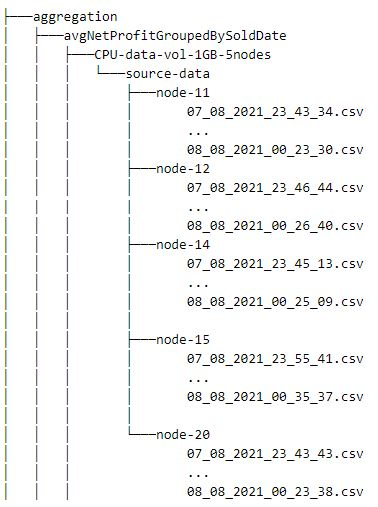
\includegraphics[scale=0.8]{figures/04-opis-danych/folder_structure.JPG}
    \caption{Struktura surowych danych}
    \label{fig:raw_file_structure}
\end{figure}
Każda funkcja została uruchomiona 25 razy per konfiguracja klastra. W każdym węźle zawarte są informacje o zużyciu procesora i pamięci RAM w trakcie wykonywania się UDF'a dla utworzonych procesów. Z tego powodu dla jednego momentu w czasie może być zaraportowanych parę procesów z ich zużyciem zasobów. Wszystko to jest zebrane w pliku CSV o następującym schemacie:
\begin{itemize}
    \item timestamp - znacznik czasowy w formacie 'rok-miesiąc-dzień godzina:minuta:sekunda.milisekunda'.
    \item PID - identyfikator procesu.
    \item CPU - procent zużycia procesora przez proces, dla zadań wielordzeniowych może przekroczyć 100\%.
    \item RAM - procent zużycia pamięci przez proces.
\end{itemize}
\section{Wstępne przetwarzanie danych}
Dane w tym stanie nie nadają się do eksperymentów, więc wpierw należało je uporządkować i zapisać w wygodnym dla nas formacie. Wpierw konieczne było pozbycie się podziału na procesy. Dla nas najbardziej interesujący jest sumaryczny przebieg zużycia zasobów na poziomie całej funkcji, a niż poszczególnych procesów. W tym celu wykorzystaliśmy bibliotekę \textbf{Pandas} często wykorzystywaną w przetwarzaniu danych. Wpisy zostały pogrupowane po znacznikach czasowych i procenty zużycia zasobów (kolumny CPU oraz RAM) zsumowane w ramach jednej grupy oraz usunięte identyfikatory procesów, gdyż nie są one nam do niczego potrzebne. Dodatkowo kolumna 'timestamp' zastąpiona jest kolumną 'epoch', która opisuje liczbę sekund (z dokładnością do 16 miejsc po przecinku) która minęła od uruchomienia funkcji.

Otrzymane zbiory zostały zapisane w takiej samej strukturze, ale w osobnym nad-folderze 'Prepared'.

W dalszym ciągu pozostaje kwestia zawartości poszczególnych folderów węzłów. Dla każdego uruchomienia funkcji posiadamy przebiegi o zużyciu w każdym węźle, zamiast ogólnie dla UDF'a. Dodatkowo bazując na pracy pilotażowej, wiemy że nie każdy więcej aktywnie brał udział w obliczeniach. Jeden z węzłów był zawsze używany jako master, którego zadaniem było zarządzanie wykonywaniem się zadań na klastrach pracujących (workers). Jeżeli master nie nadał zadania każdemu z klastrów pracujących, to taki węzeł nic nie robił poza wysyłaniem okazyjnie informacji o stanie (tzn. czy jest wciąż aktywny). Z tego powodu następnym krokiem było odfiltrowanie wszystkich węzłów bezczynnych oraz mastera i zachowanie jednie tych, które wykonywały jakieś obliczenia.

Założyliśmy, że master, ze względu na to, że nie wykonuje pracy na danych nie powinien wykorzystywać zbyt dużo pamięci RAM. I faktycznie dla każdego eksperymentu można było znaleźć jeden węzeł, którego średnie zużycie RAM było wyraźnie mniejsze. Eksperymentując ustaliliśmy próg 2\% - odrzuciliśmy wszystkie węzły, dla których średnie zużycie RAM było poniżej tego progu.

Następnym krokiem było znalezienie i wykluczenie węzłów niepracujących. Jako, że takie węzły wysyłały tylko okazyjne informacje o tym, że wciąż są aktywne to różnice między zużyciem CPU dla nich i dla węzłów pracujących również były wyraźnie widoczne. Dokładnie to było widać zwłaszcza w kilku początkowych pomiarach, które dla węzłów pracujących charakteryzowały się wysokim zużyciem CPU, co było dokładnie opisane i wytłumaczone w pracy pilotażowej. Z tego względu odrzuciliśmy węzły, których początkowe pomiary były niskie.

Ostatecznie chcieliśmy również uzyskać jak najmniej plików wejściowych, aby ułatwić dalsze przetwarzanie danych. Inspirując się przykładowym zbiorem danych wykorzystywanym do uczenia maszynowego na danych typu Time Series, utworzyliśmy pojedyncze pliki CSV per typ funkcji UDF o następującym schemacie:
\begin{itemize}
    \item snapshot - identyfikator pojedynczego przebiegu czasowego.
    \item label - opis typu funkcji, np 'aggregation'.
    \item udf - nazwa funkcji z którego pochodzi danych przebieg czasowy.
    \item epoch - liczba sekund, która minęła od uruchomienia się funkcji z dokładnością do 16 miejsc po przecinku.
    \item CPU - procent zużycia procesora przez proces, dla zadań wielordzeniowych może przekroczyć 100\%.
    \item RAM - procent zużycia pamięci przez proces.
\end{itemize}
Poniżej znajduje się przykładowe parę wierszy z tak utworzonego pliku dla funkcji typu 'aggregation':
\begin{table}[H]
\center{
 \begin{tabular}{|c|c|c|c|c|c|} 
 \hline
snapshot & label & udf & epoch & CPU & RAM \\
\hline
0 & aggregation & avgNetProfitGroupedBySoldDate & 0.0 & 206.7 & 4.8 \\
\hline
0 & aggregation & avgNetProfitGroupedBySoldDate & 0.1562700271606445 & 220.0 & 5.0 \\
\hline
0 & aggregation & avgNetProfitGroupedBySoldDate & 0.3140101432800293 & 133.3 & 5.19 \\
\hline
0 & aggregation & avgNetProfitGroupedBySoldDate & 0.4715931415557861 & 146.7 & 5.3 \\
\hline
0 & aggregation & avgNetProfitGroupedBySoldDate & 0.6280381679534912 & 126.7 & 5.4 \\
\hline
0 & aggregation & avgNetProfitGroupedBySoldDate & 0.7846581935882568 & 160.0 & 5.5 \\
\hline
\end{tabular}
}
\caption{Początek pliku joined\_aggregation.csv}
\end{table}

Zebrane tak dane mogą zostać użyte w dalszym przetwarzaniu. W zbiorze możemy wyróżnić pięć typów funkcji zależnie od rodzaju przetwarzania:
\begin{itemize}
    \item aggregation
    \item filtration
    \item filtration-aggregation
    \item filtration-aggregation-join
    \item filtration-join
\end{itemize}
Kolumna 'label' zawiera jedną z tych wartości, poniżej w celu przedstawienia przykładowych przebiegów czasowych narysowane są wykresy dla każdego z typów z podziałem na RAM i CPU.

\begin{figure}[H]
  \centering
  \subfloat[CPU]{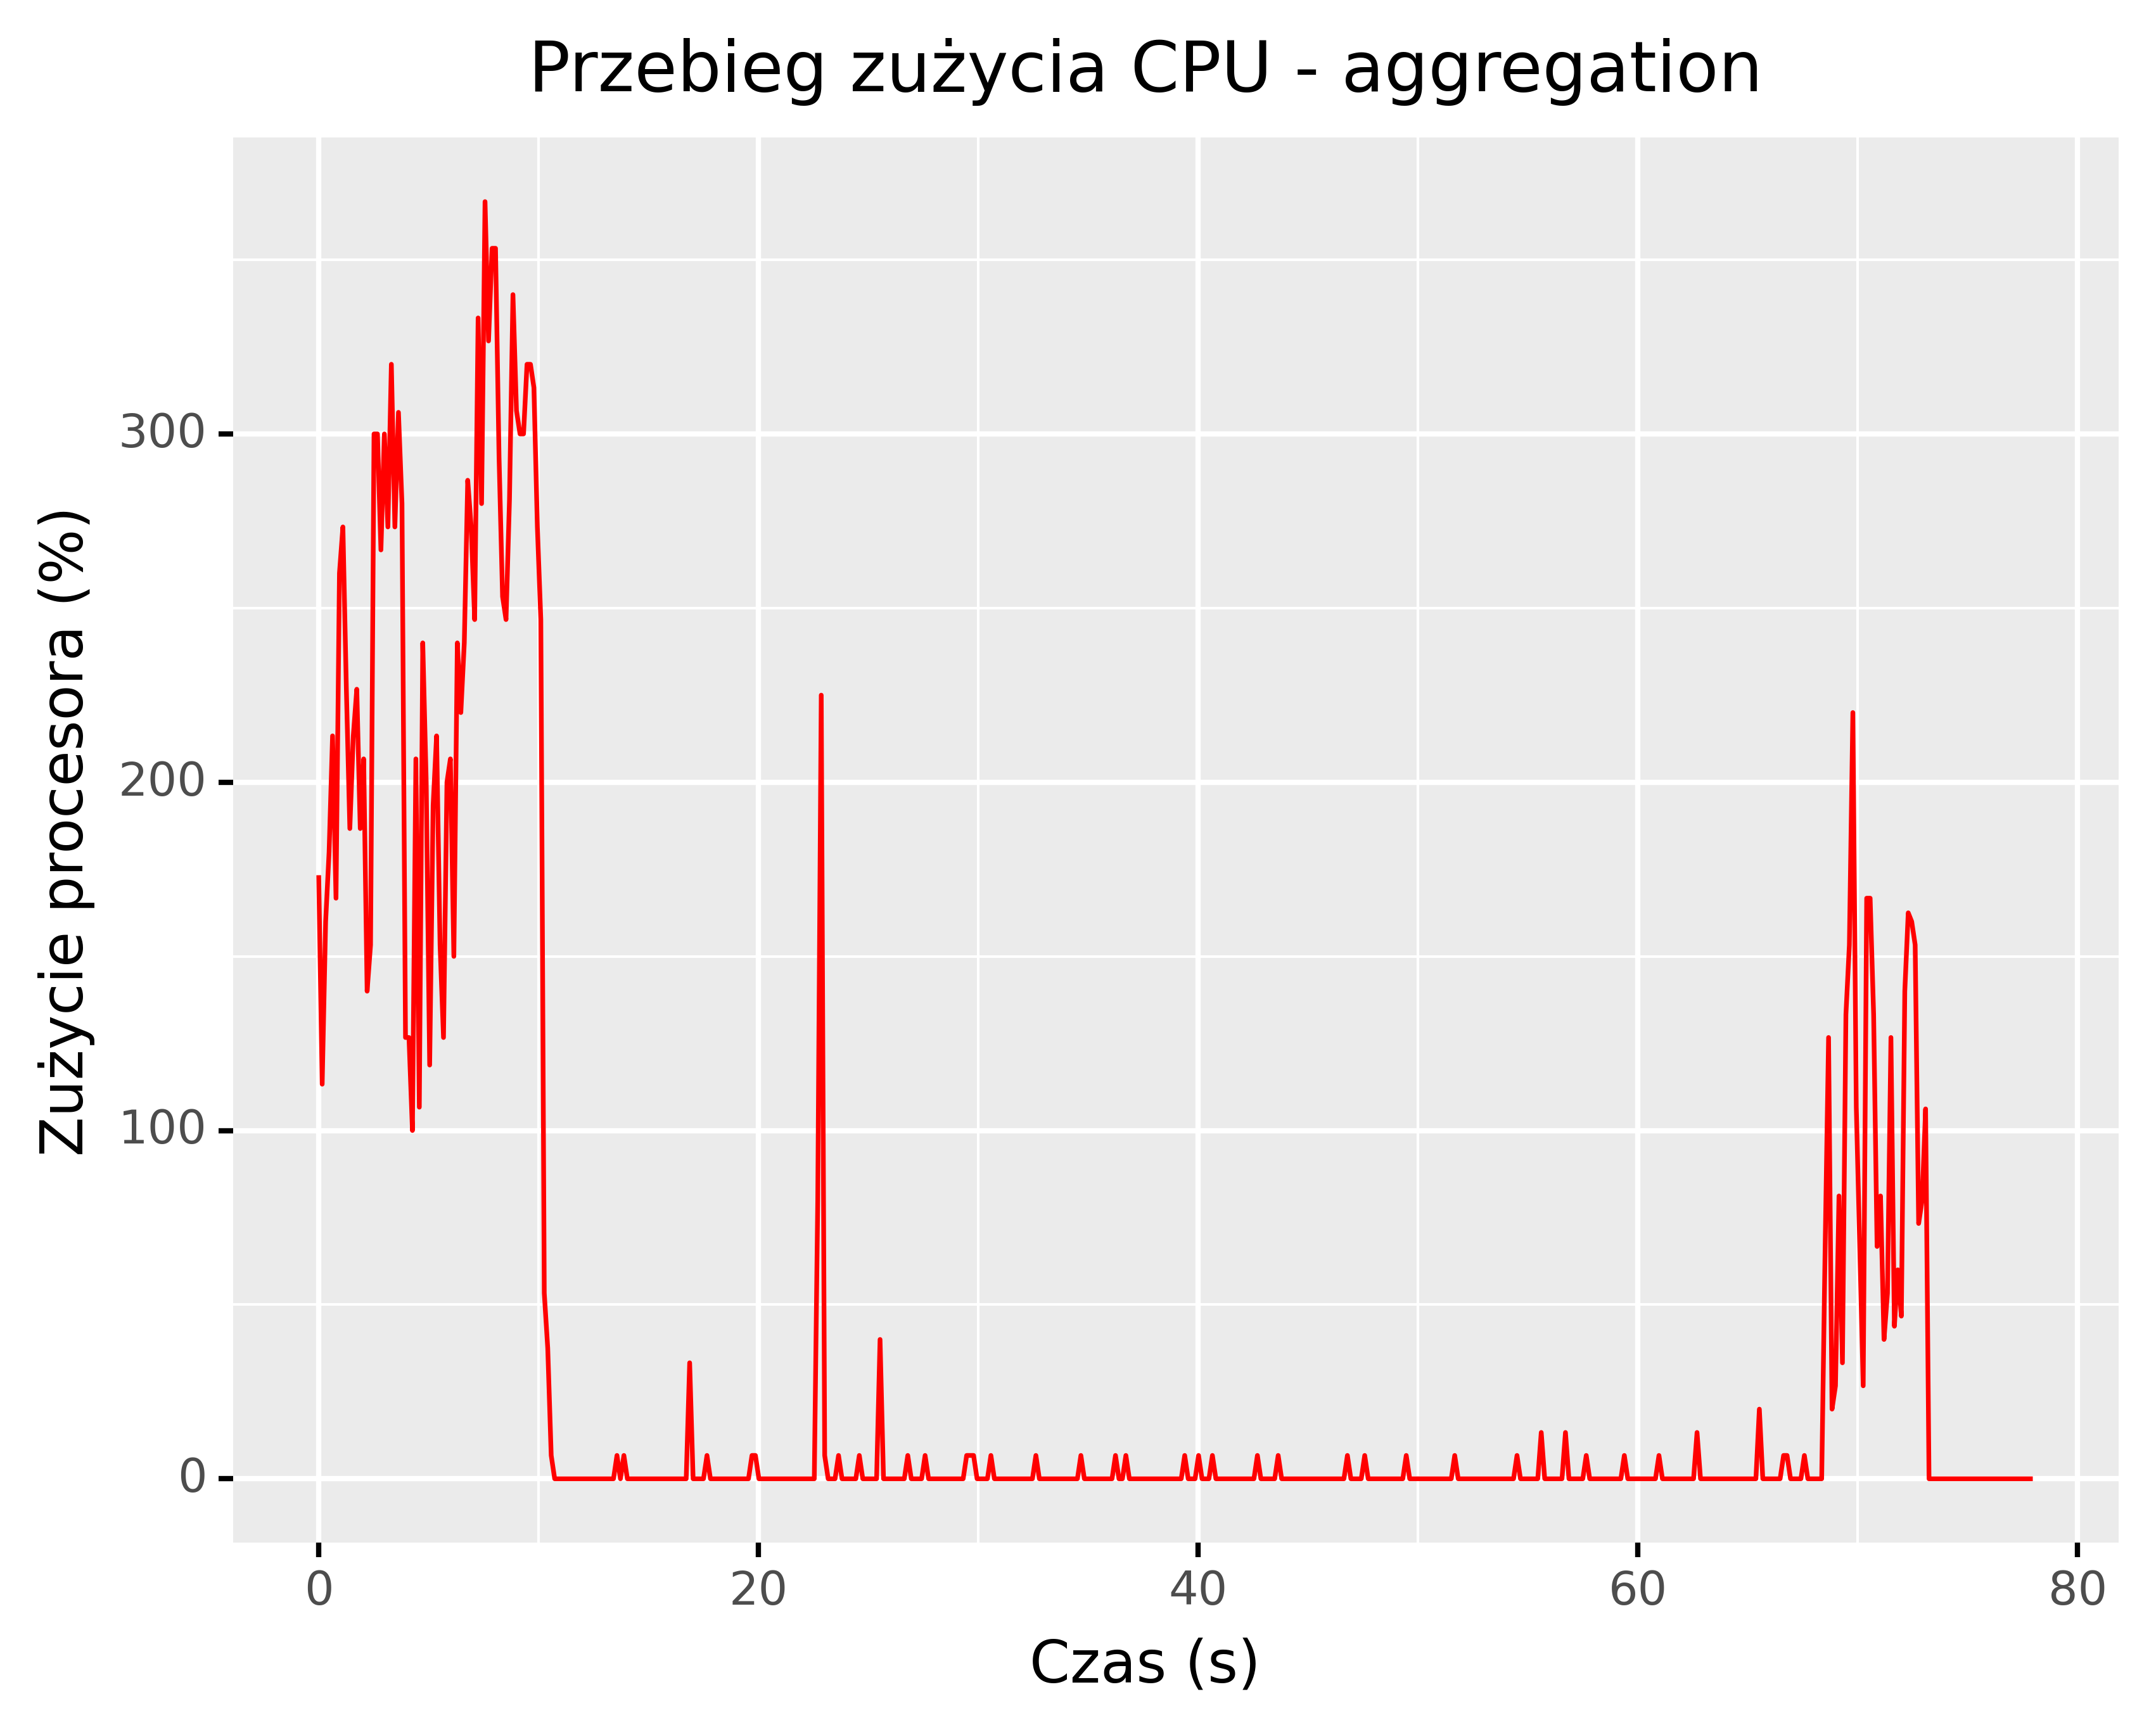
\includegraphics[width=0.5\textwidth]{figures/04-opis-danych/aggregation_example_cpu_snapshot_1.png}\label{aggregation_example:f1}}
  \hfill
  \subfloat[RAM]{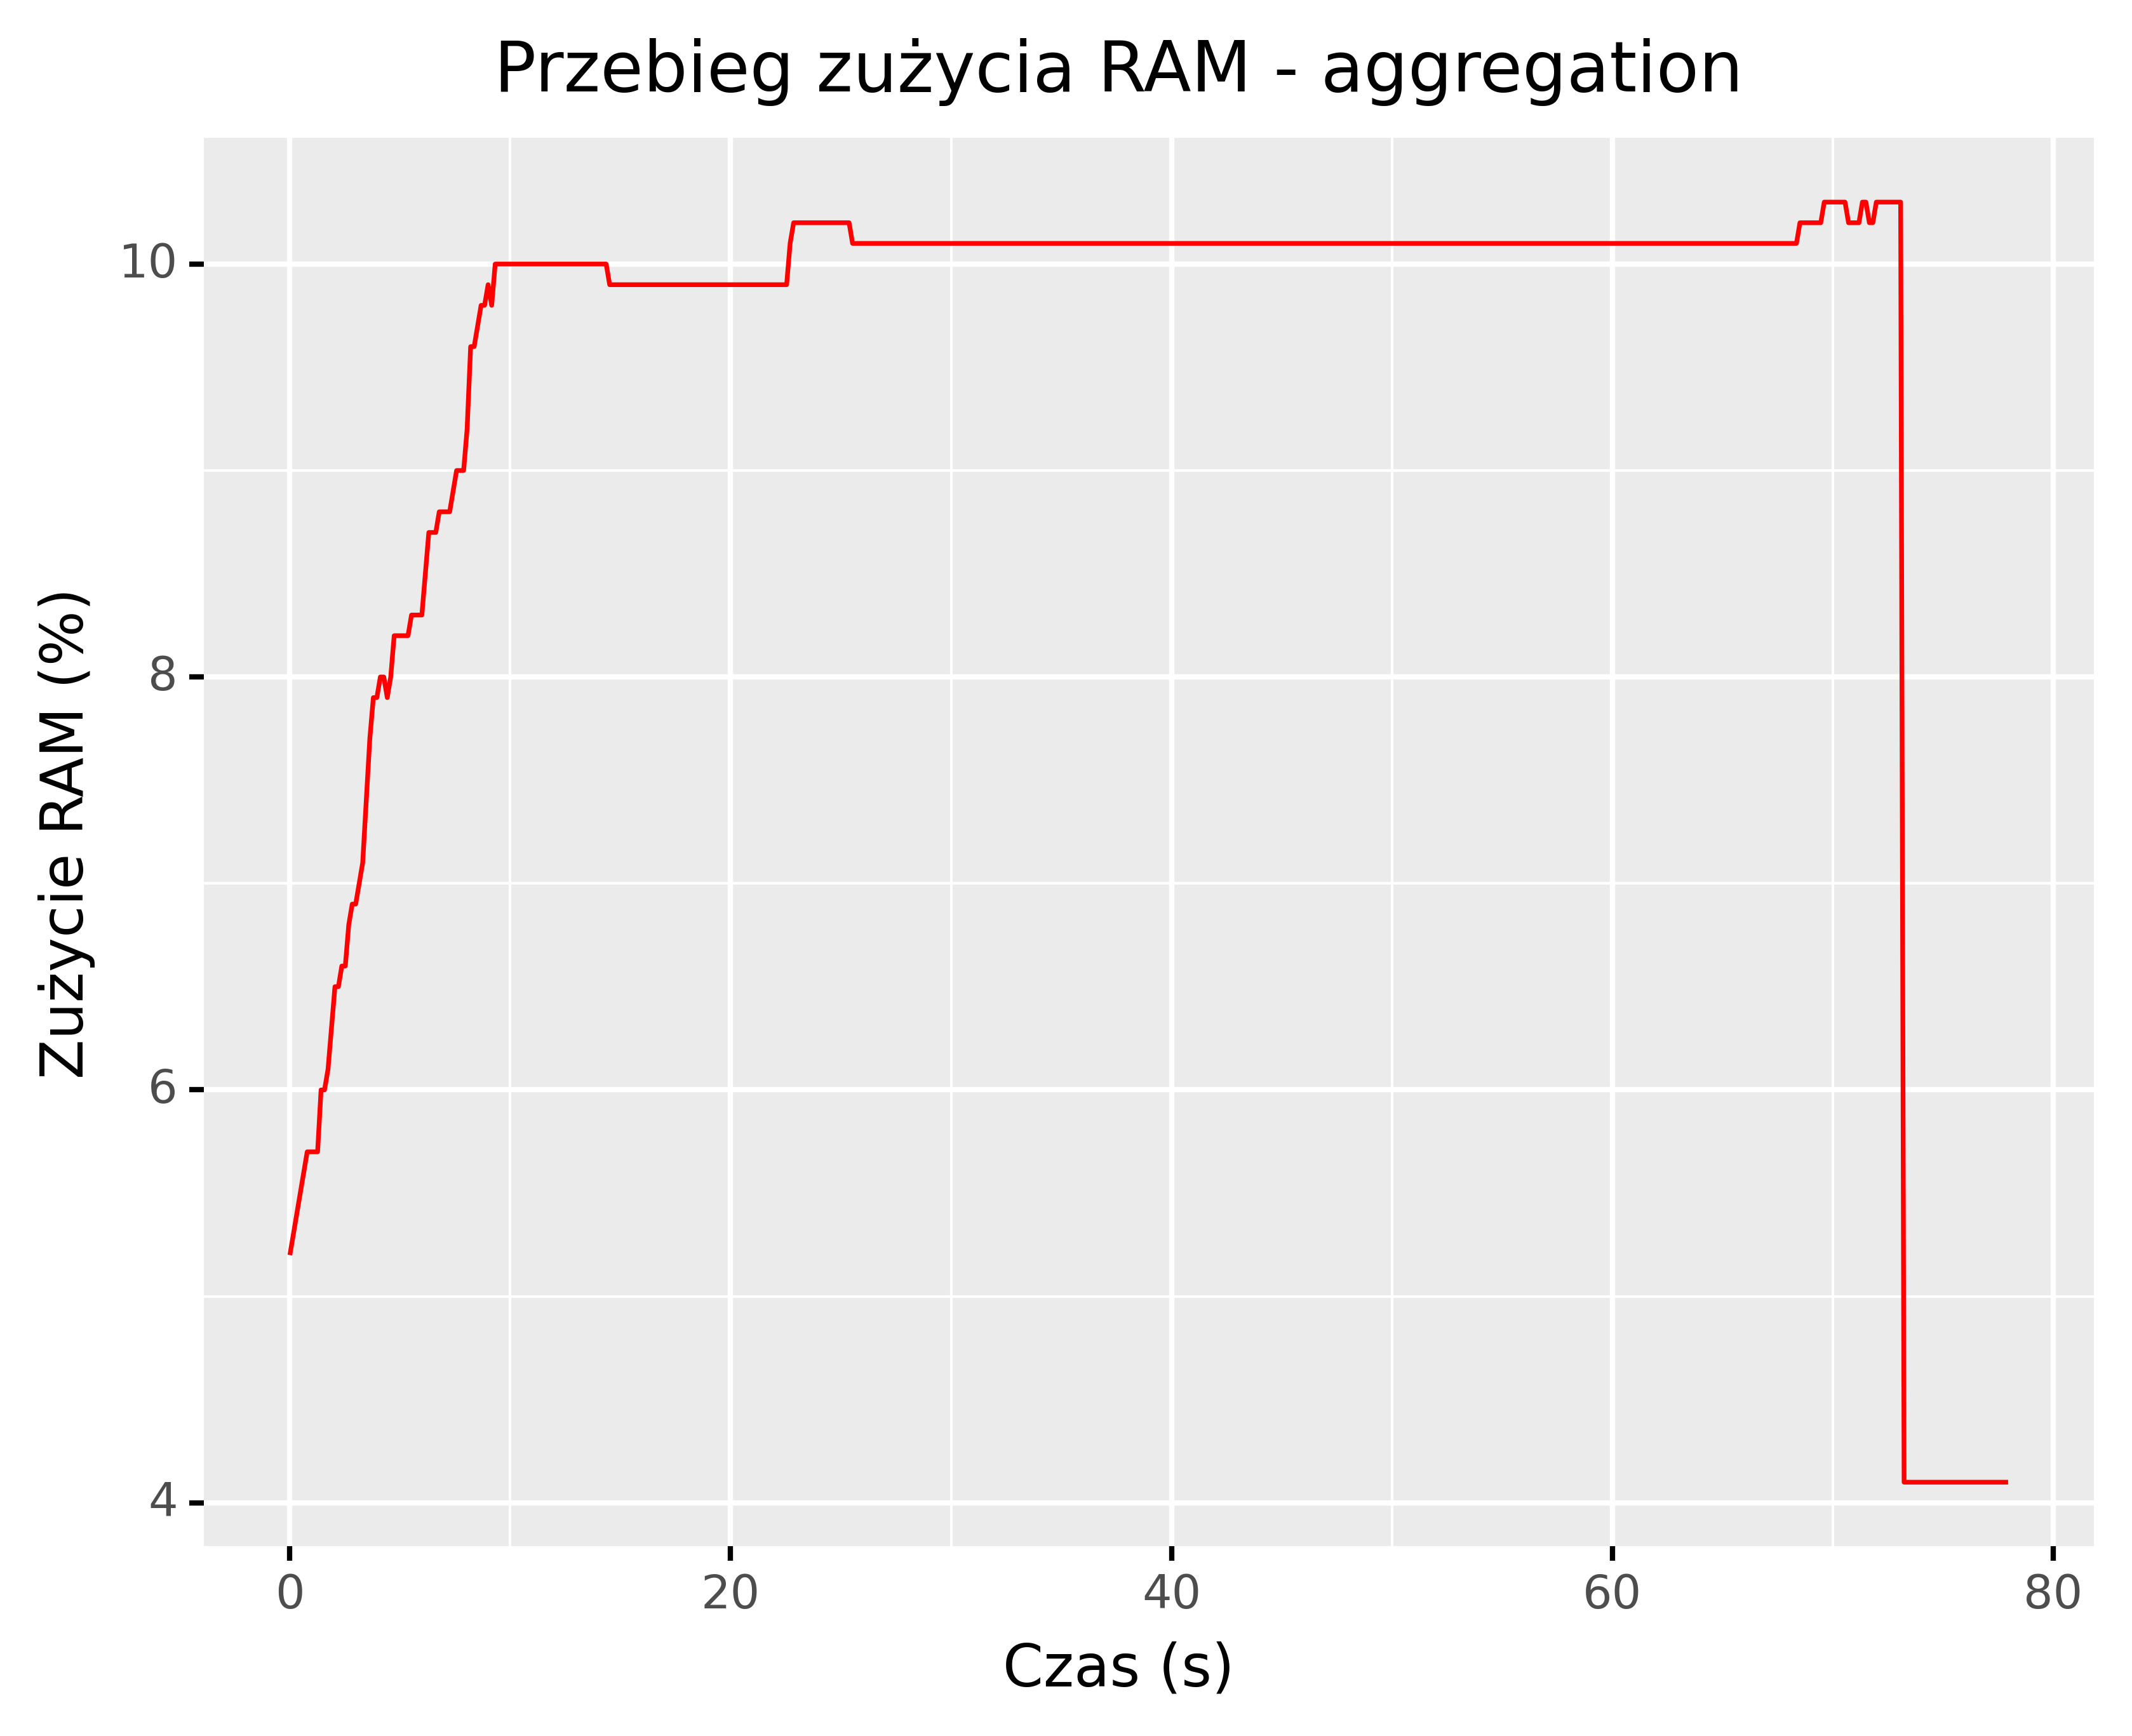
\includegraphics[width=0.5\textwidth]{figures/04-opis-danych/aggregation_example_ram_snapshot_1.png}\label{aggregation_example:f2}}
  \caption{Przykładowy przebieg zużycia zasobów dla agregacji (snapshot = 1)}
  \label{aggregation_example}
\end{figure}

\begin{figure}[H]
  \centering
  \subfloat[CPU]{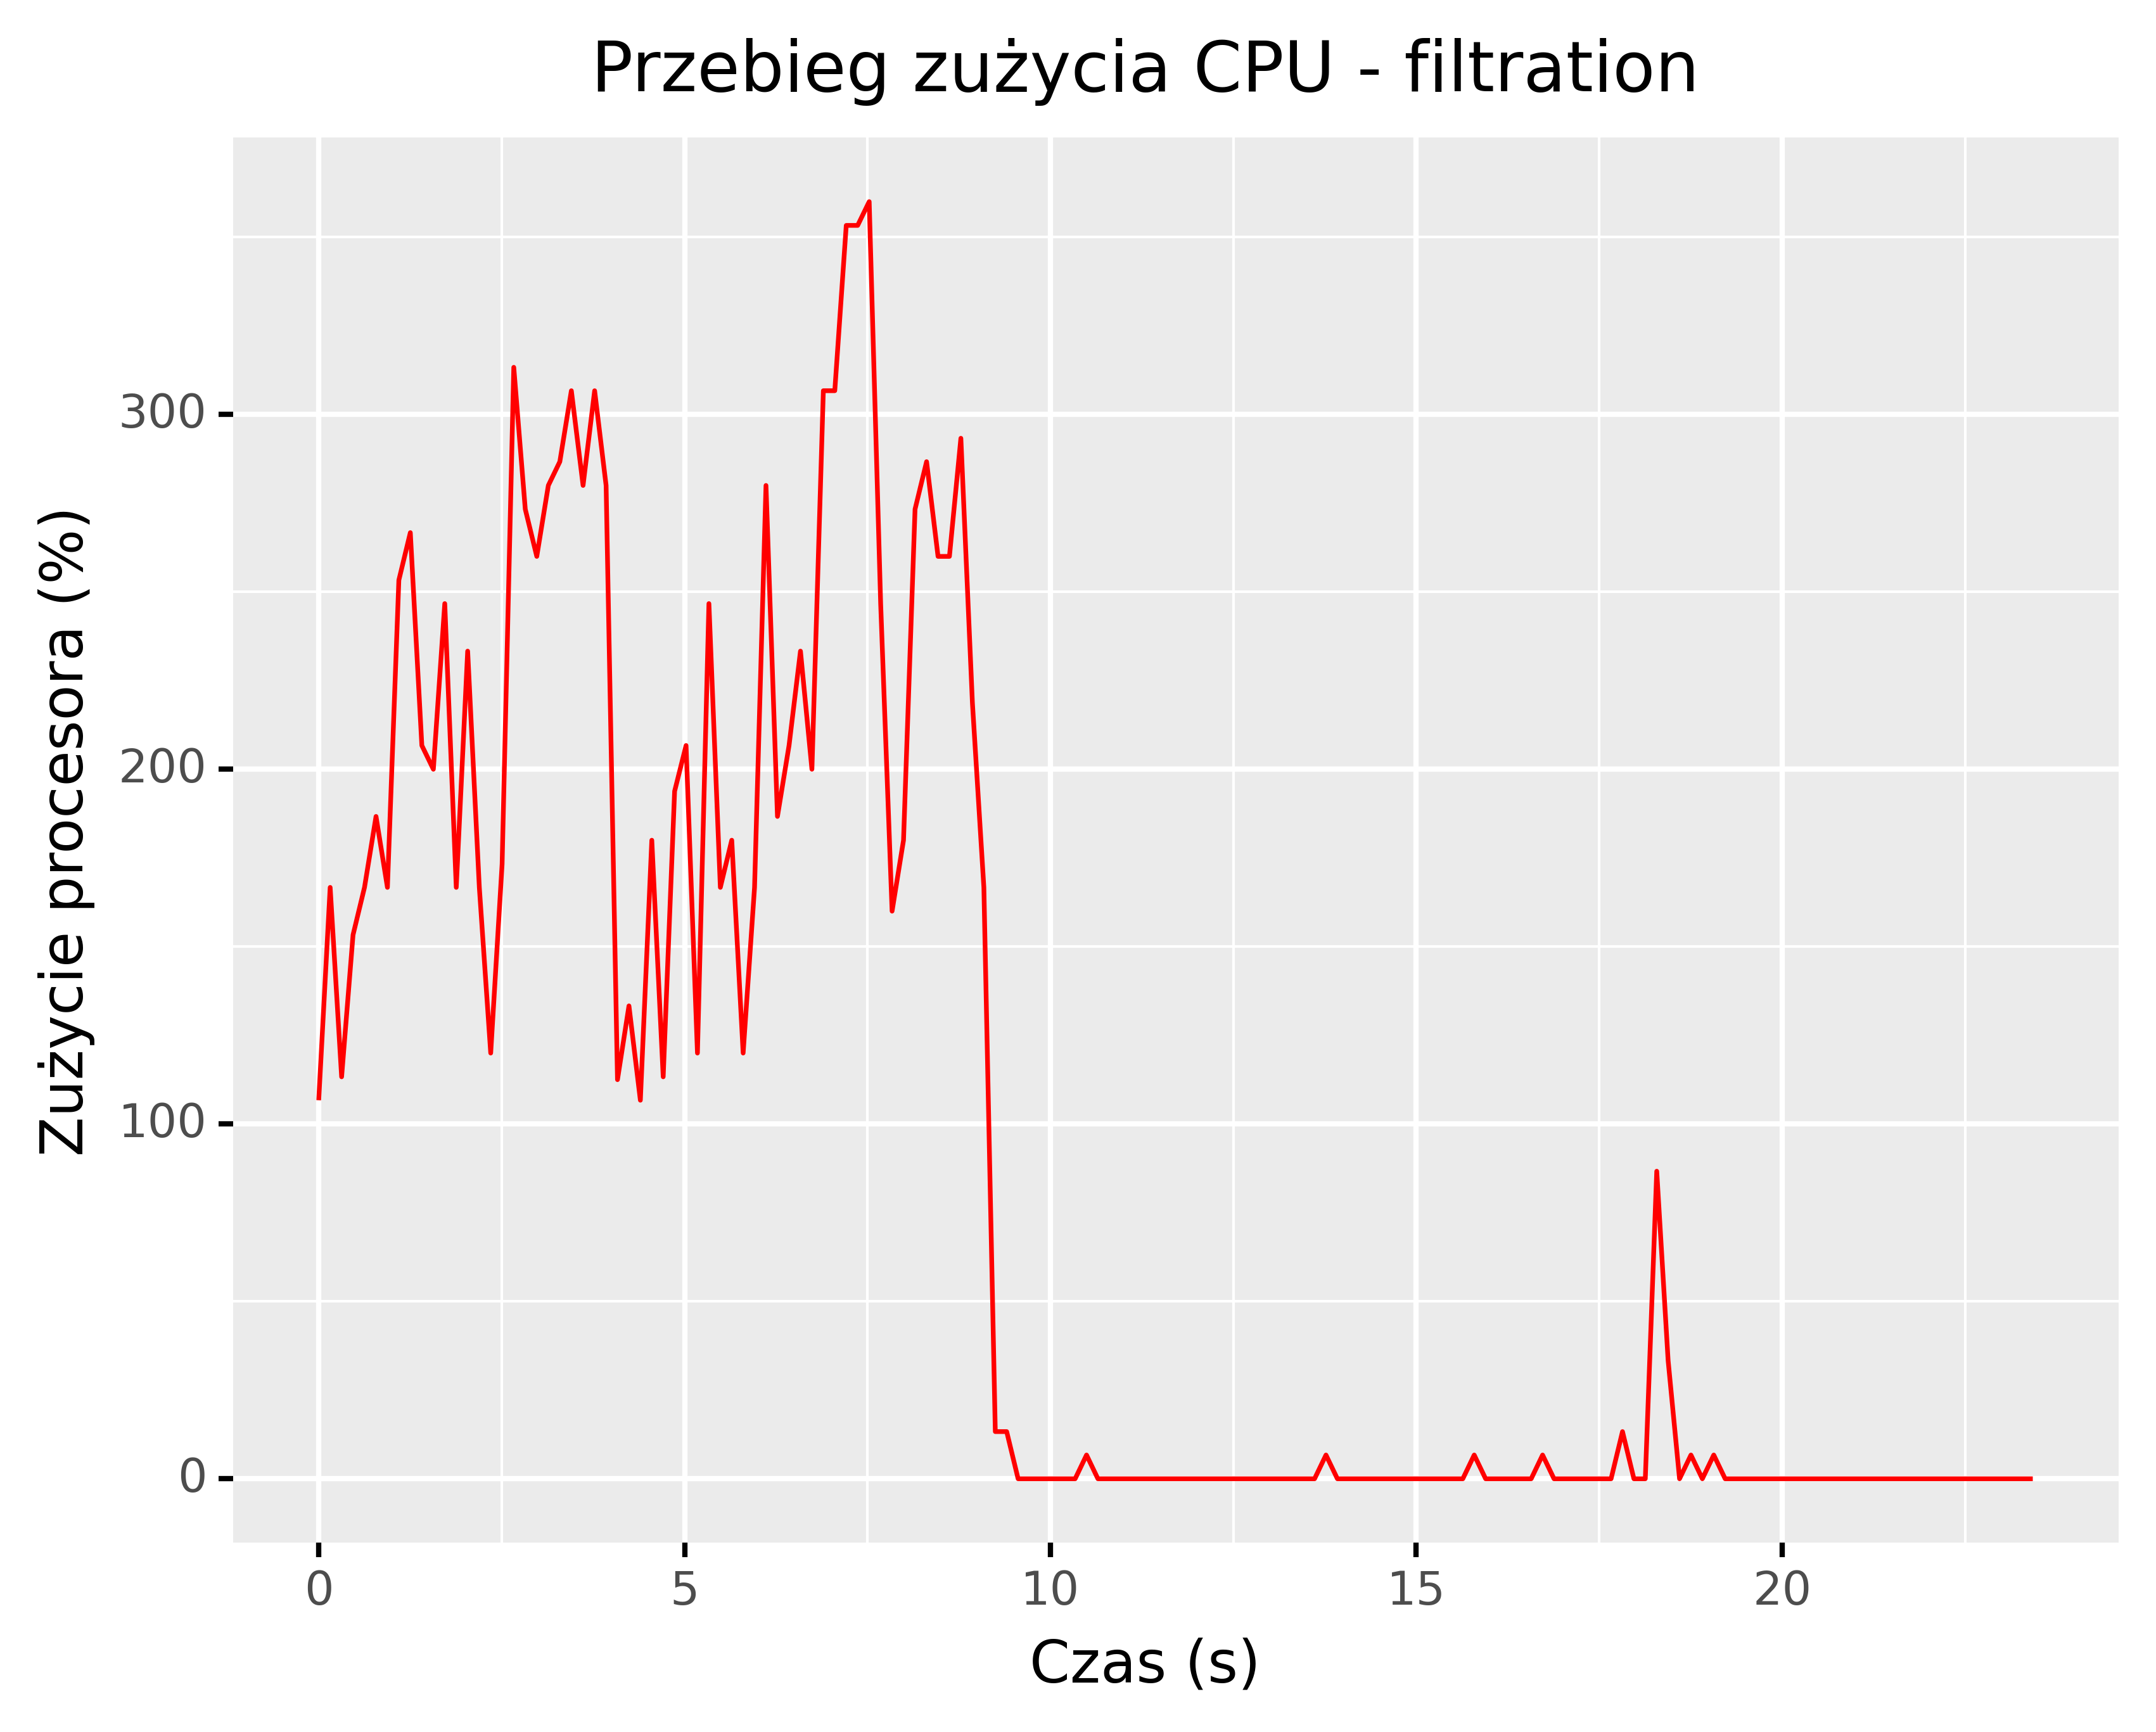
\includegraphics[width=0.5\textwidth]{figures/04-opis-danych/filtration_example_cpu_snapshot_1.png}\label{filtration:f1}}
  \hfill
  \subfloat[RAM]{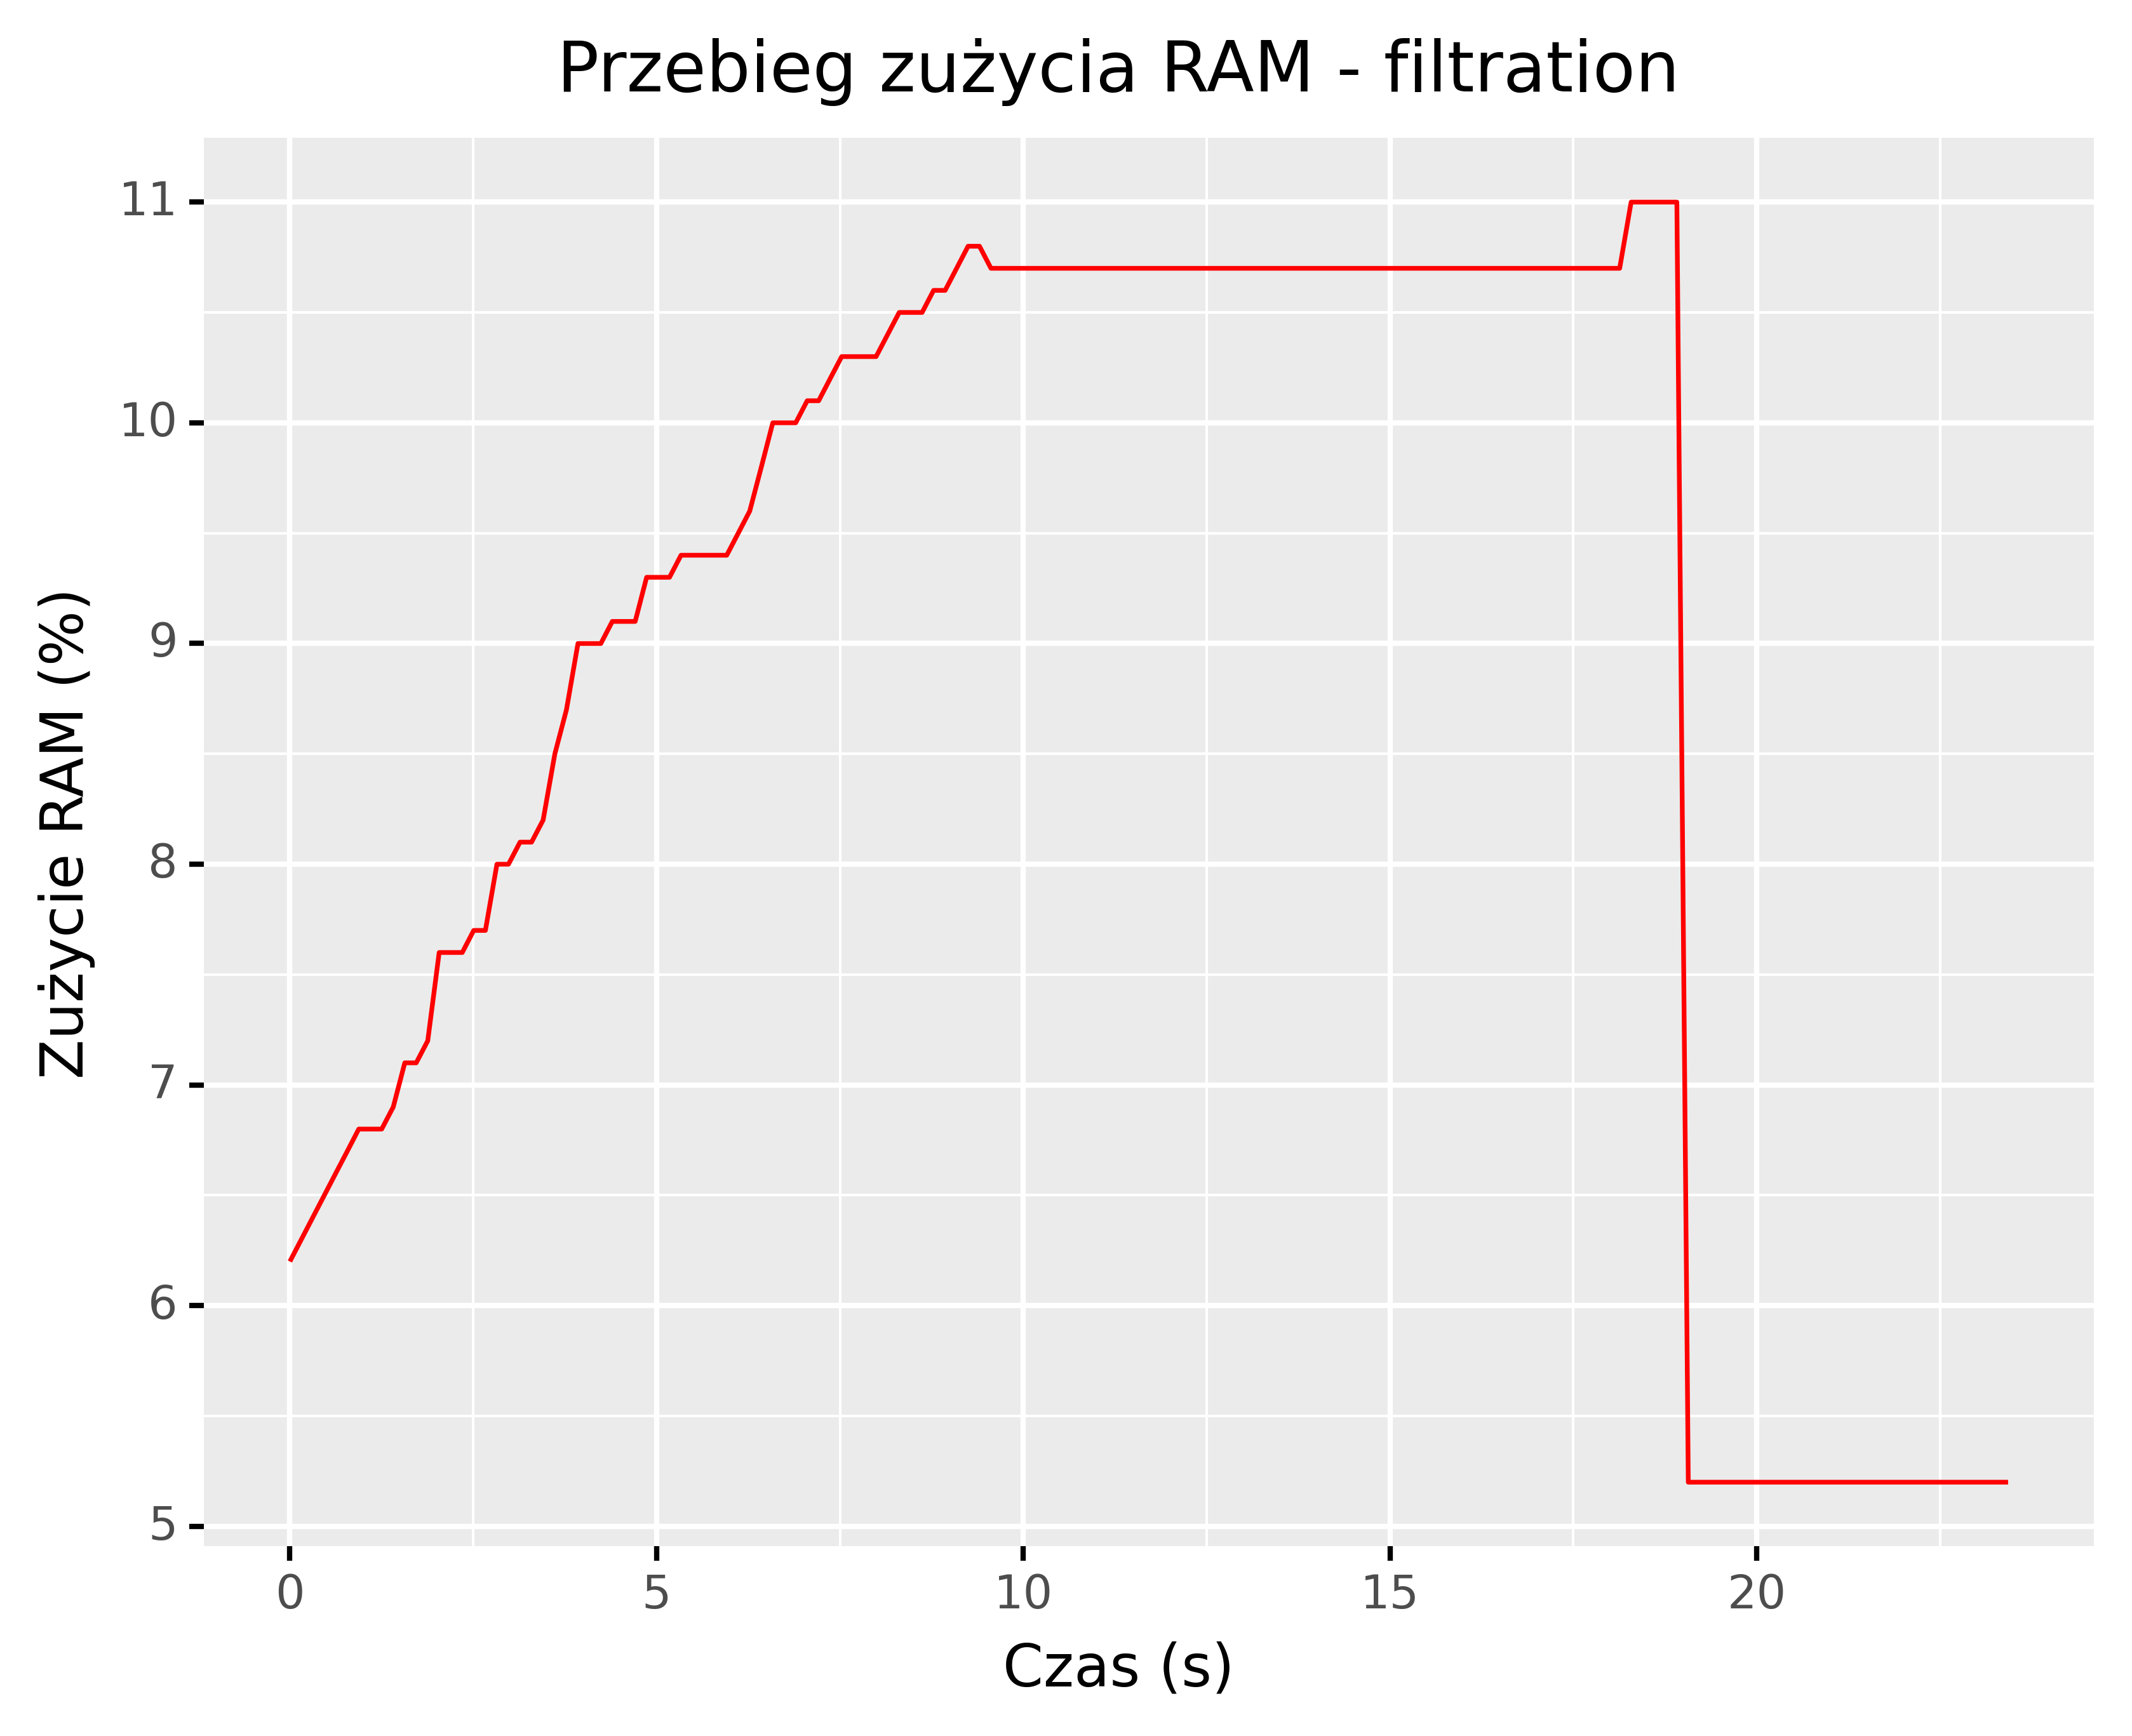
\includegraphics[width=0.5\textwidth]{figures/04-opis-danych/filtration_example_ram_snapshot_1.png}\label{filtration:f2}}
  \caption{Przykładowy przebieg zużycia zasobów dla filtracji (snapshot = 1)}
  \label{filtration_example}
\end{figure}

\begin{figure}[H]
  \centering
  \subfloat[CPU]{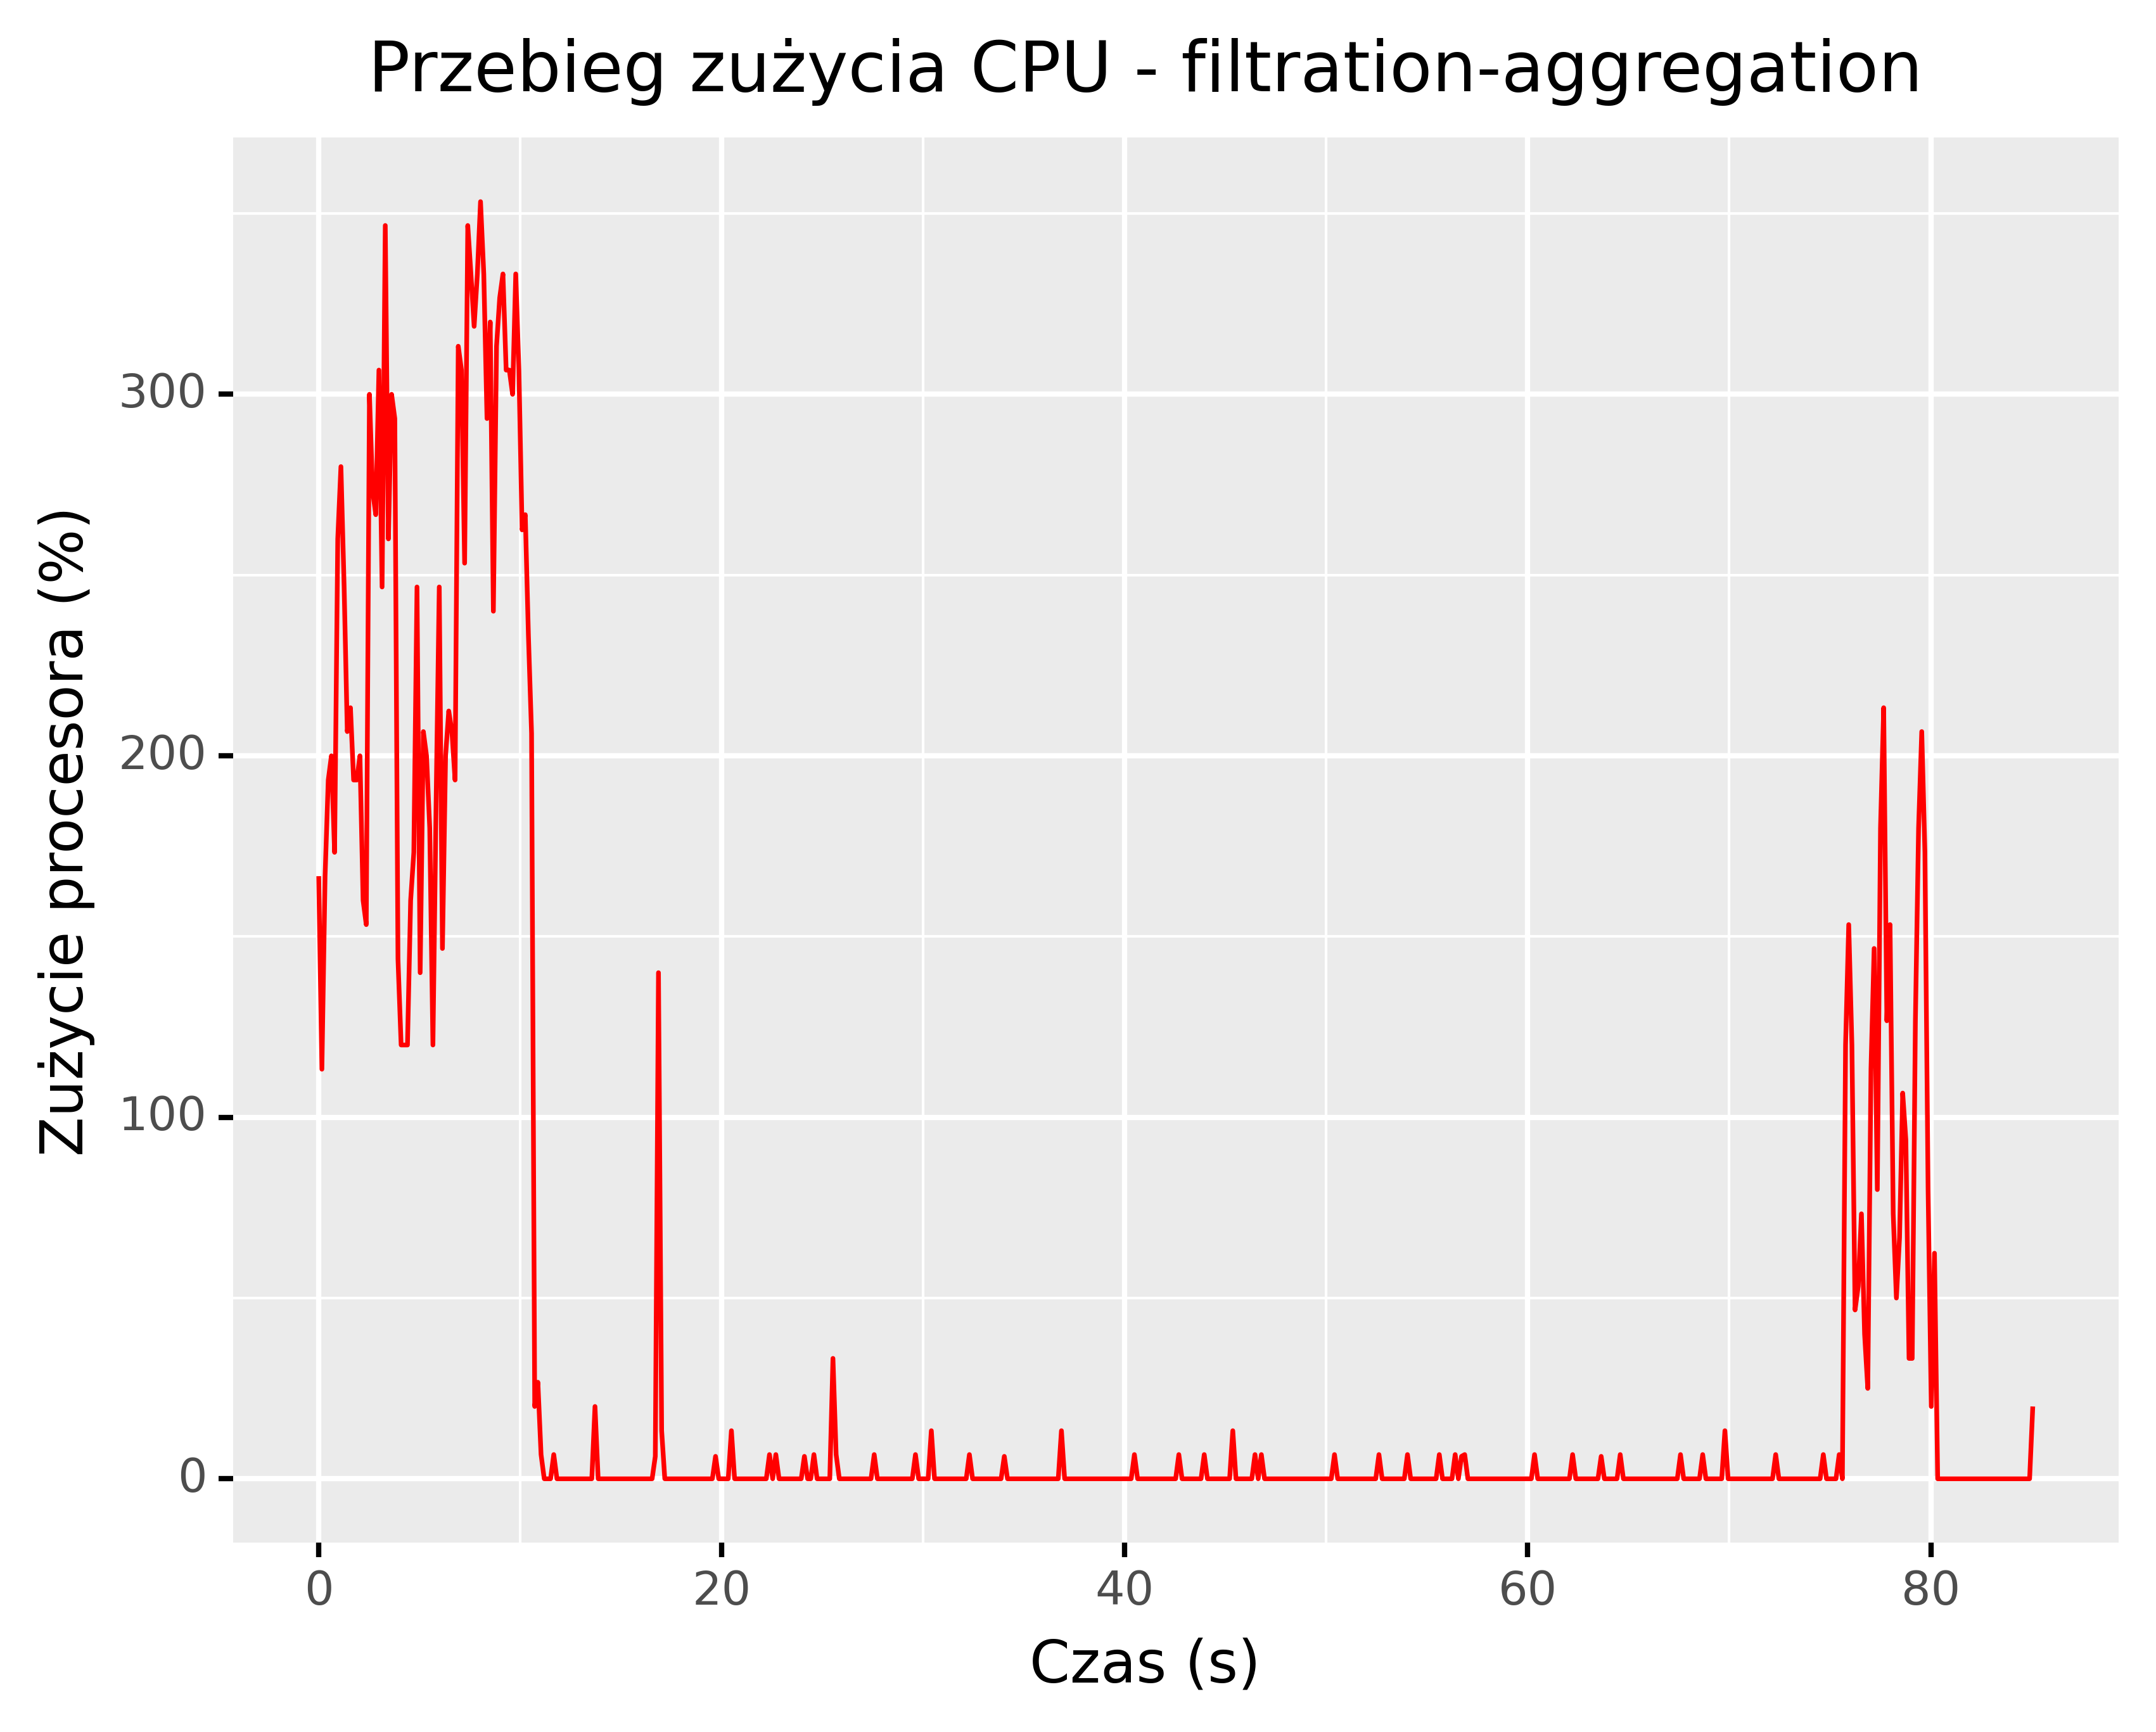
\includegraphics[width=0.5\textwidth]{figures/04-opis-danych/filtration-aggregation_example_cpu_snapshot_1.png}\label{filtration-aggregation:f1}}
  \hfill
  \subfloat[RAM]{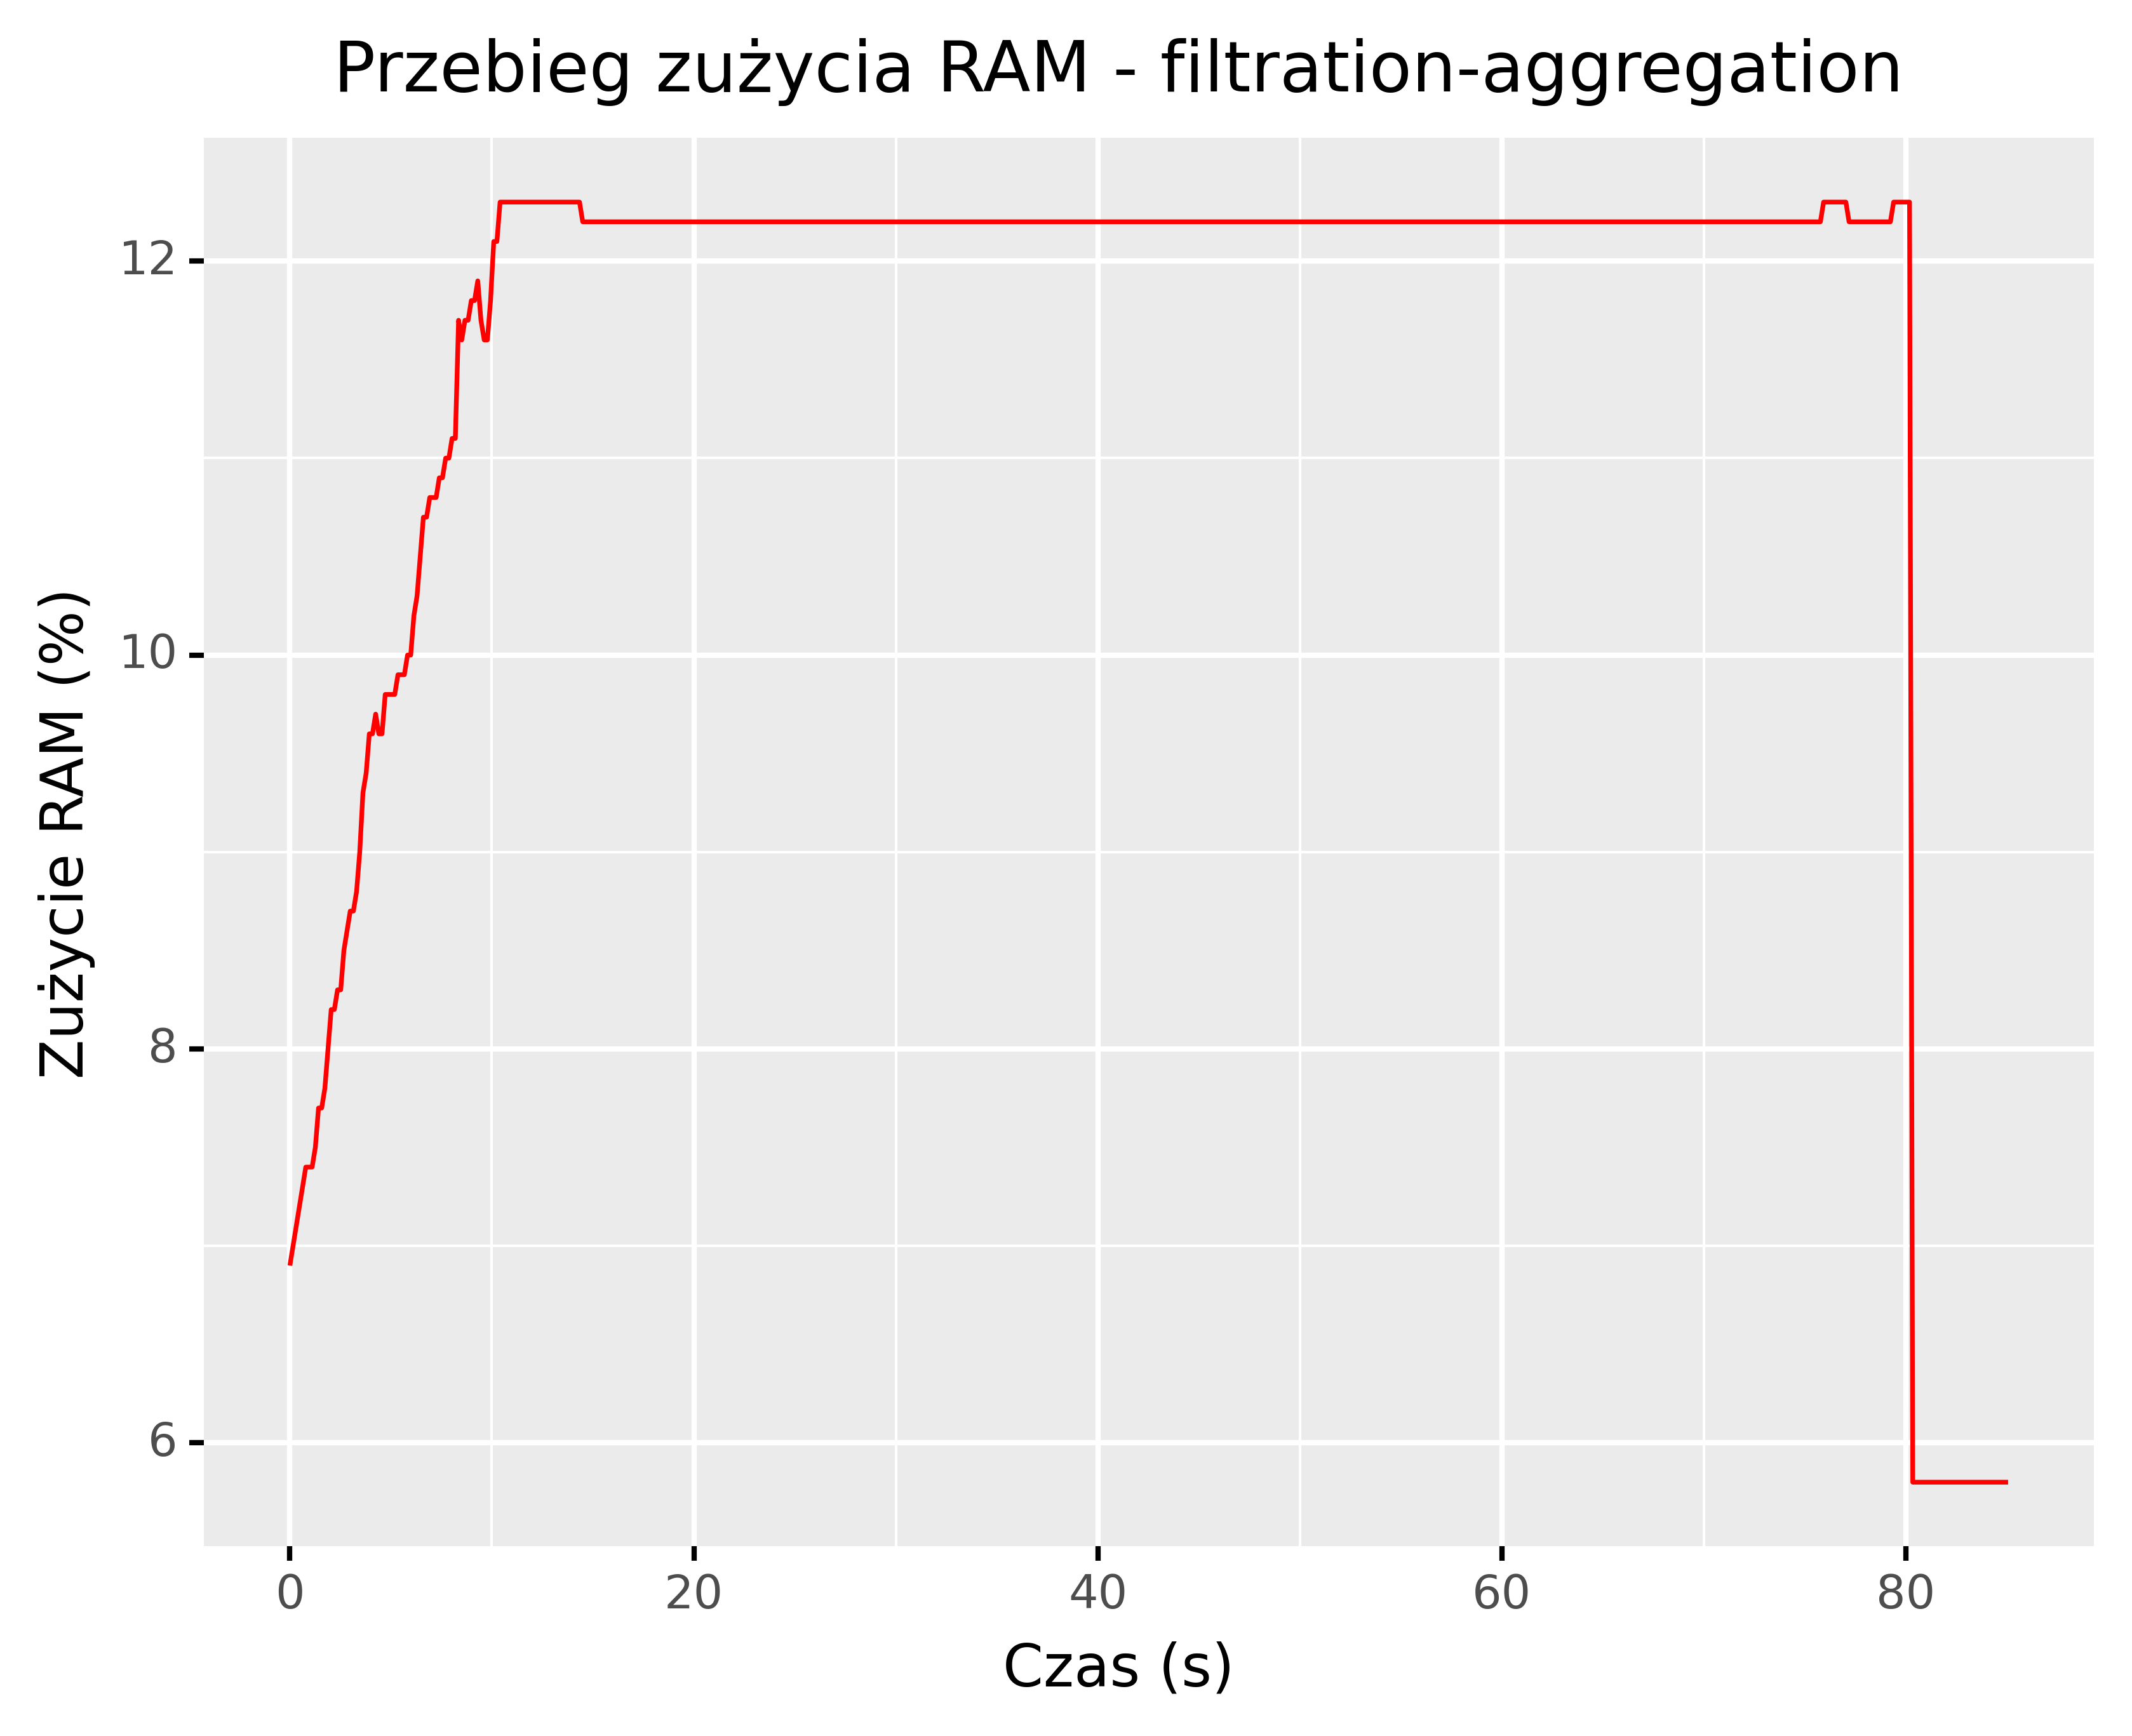
\includegraphics[width=0.5\textwidth]{figures/04-opis-danych/filtration-aggregation_example_ram_snapshot_1.png}\label{filtration-aggregation:f2}}
  \caption{Przykładowy przebieg zużycia zasobów dla filtracjo-agregacji (snapshot = 1)}
  \label{filtration-aggregation_example}
\end{figure}

\begin{figure}[H]
  \centering
  \subfloat[CPU]{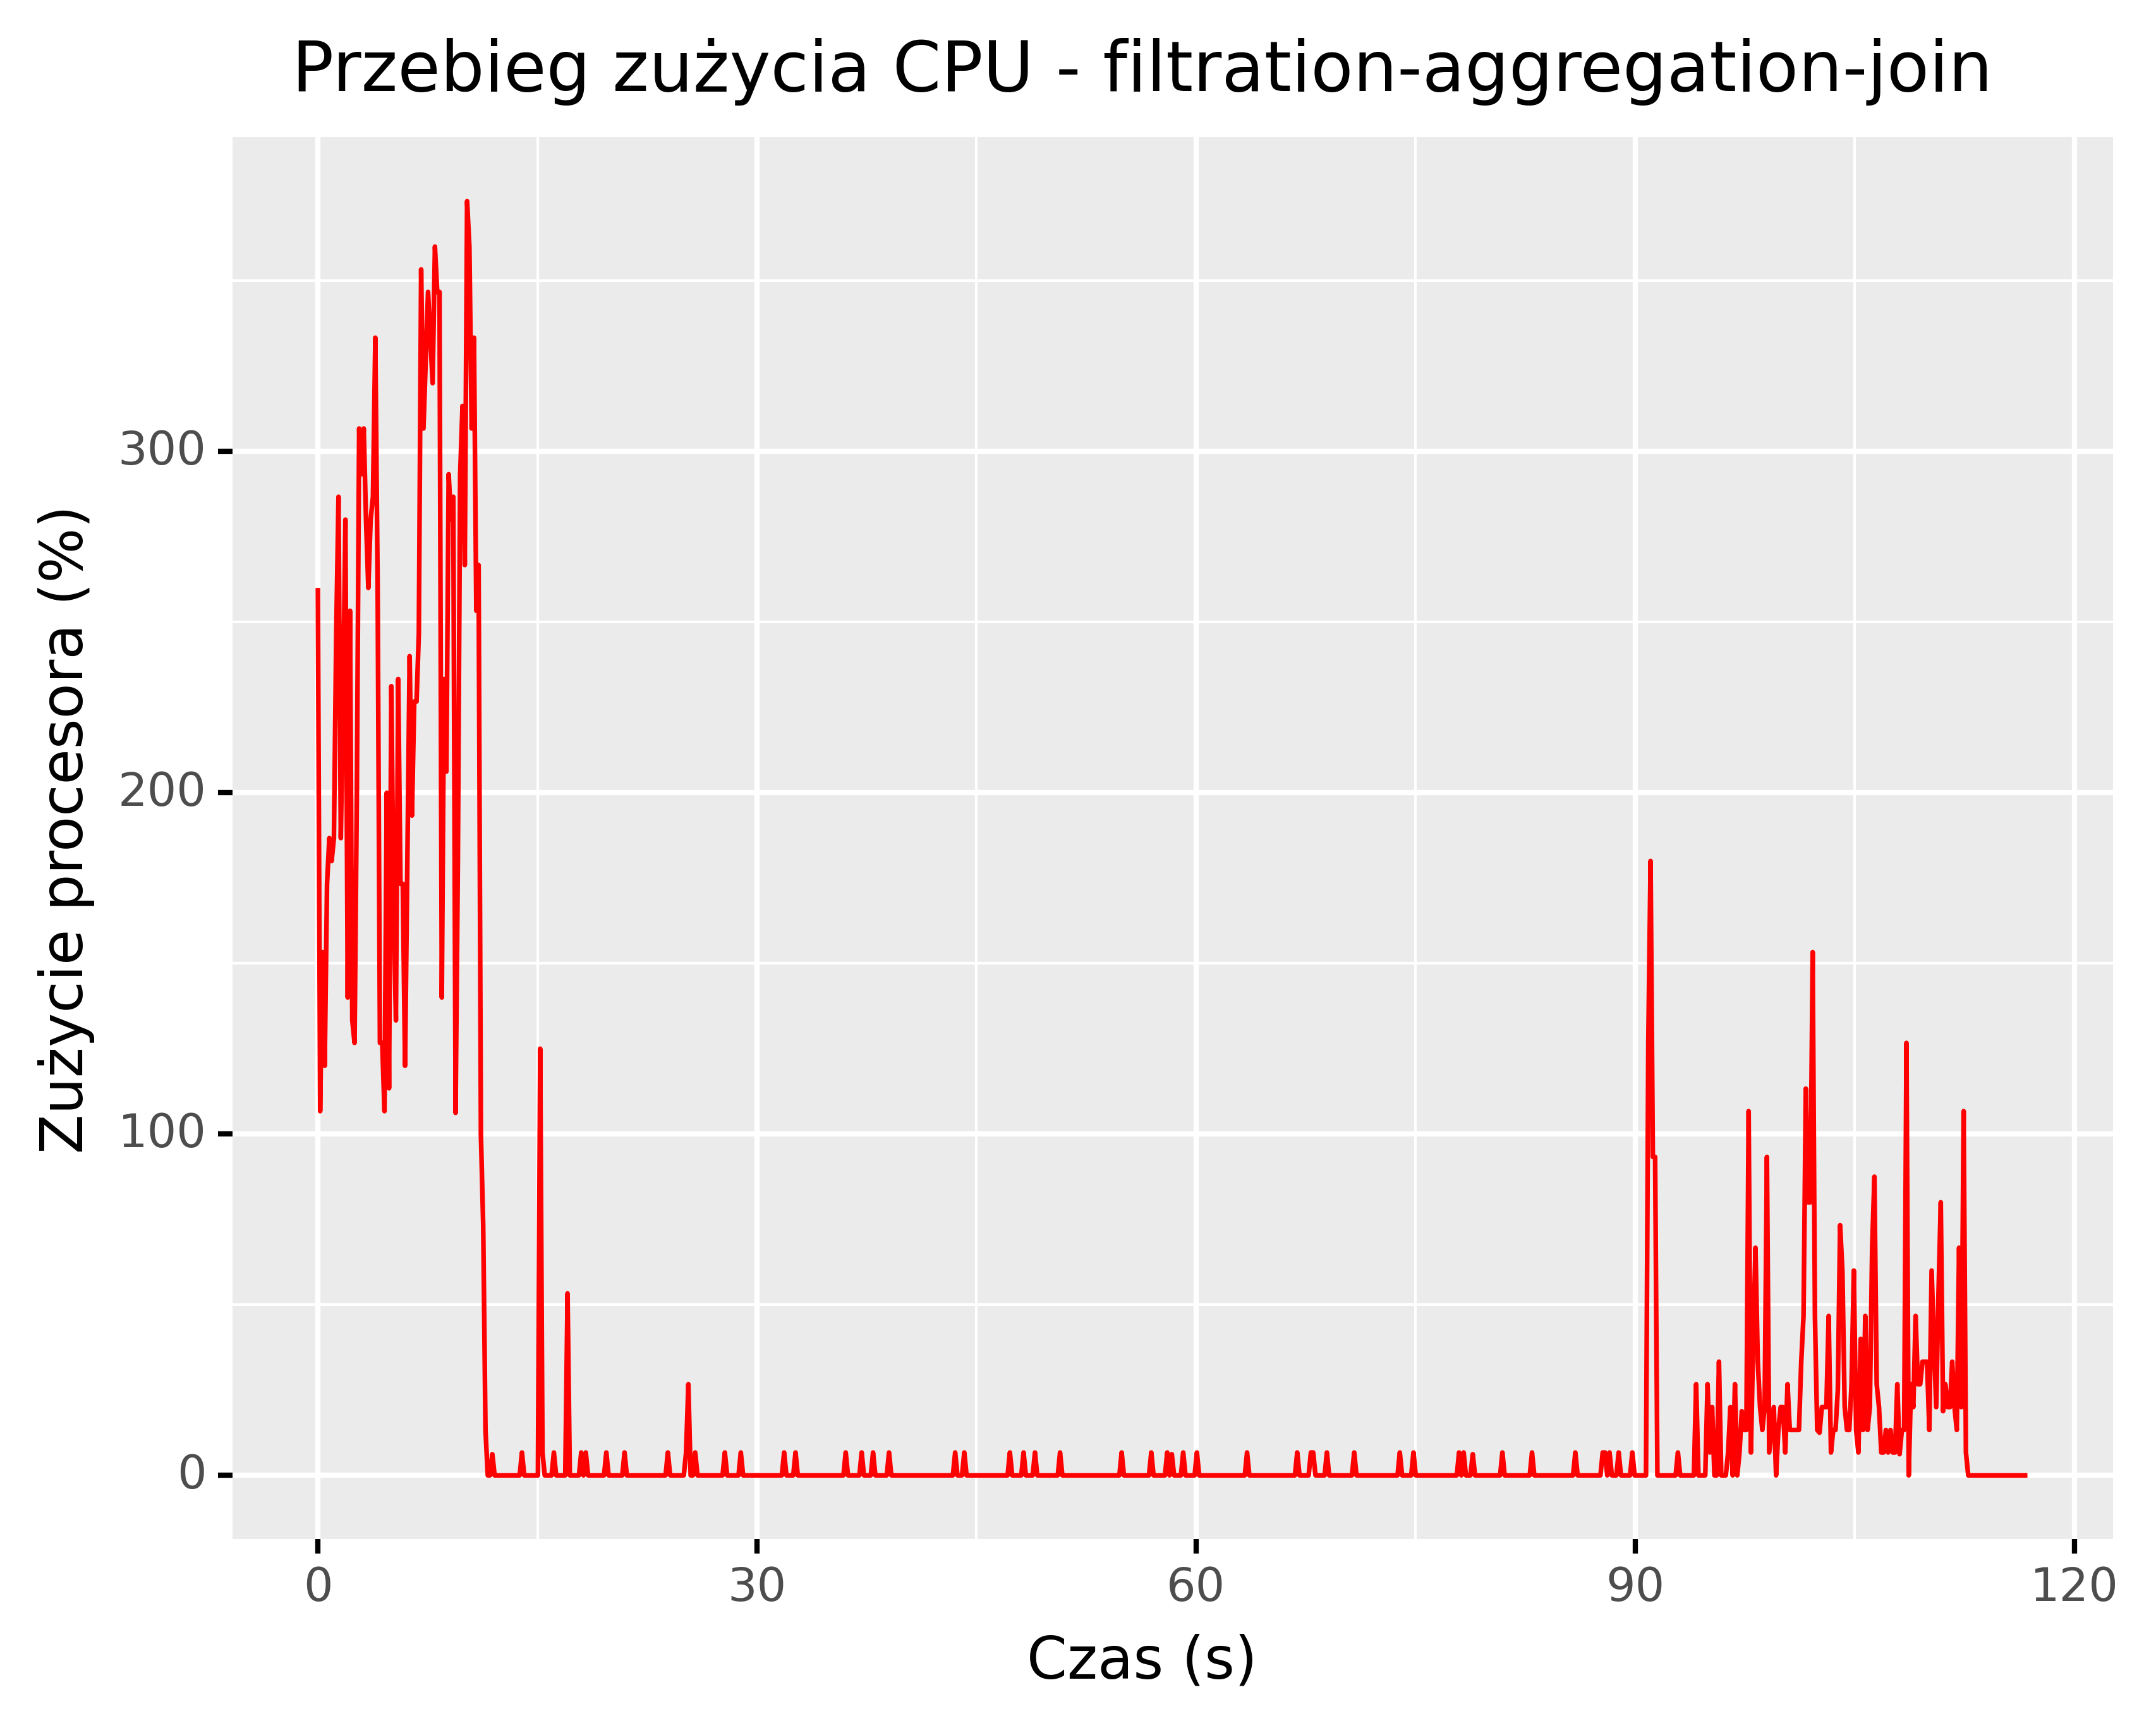
\includegraphics[width=0.5\textwidth]{figures/04-opis-danych/filtration-aggregation-join_example_cpu_snapshot_1.png}\label{filtration-aggregation-join:f1}}
  \hfill
  \subfloat[RAM]{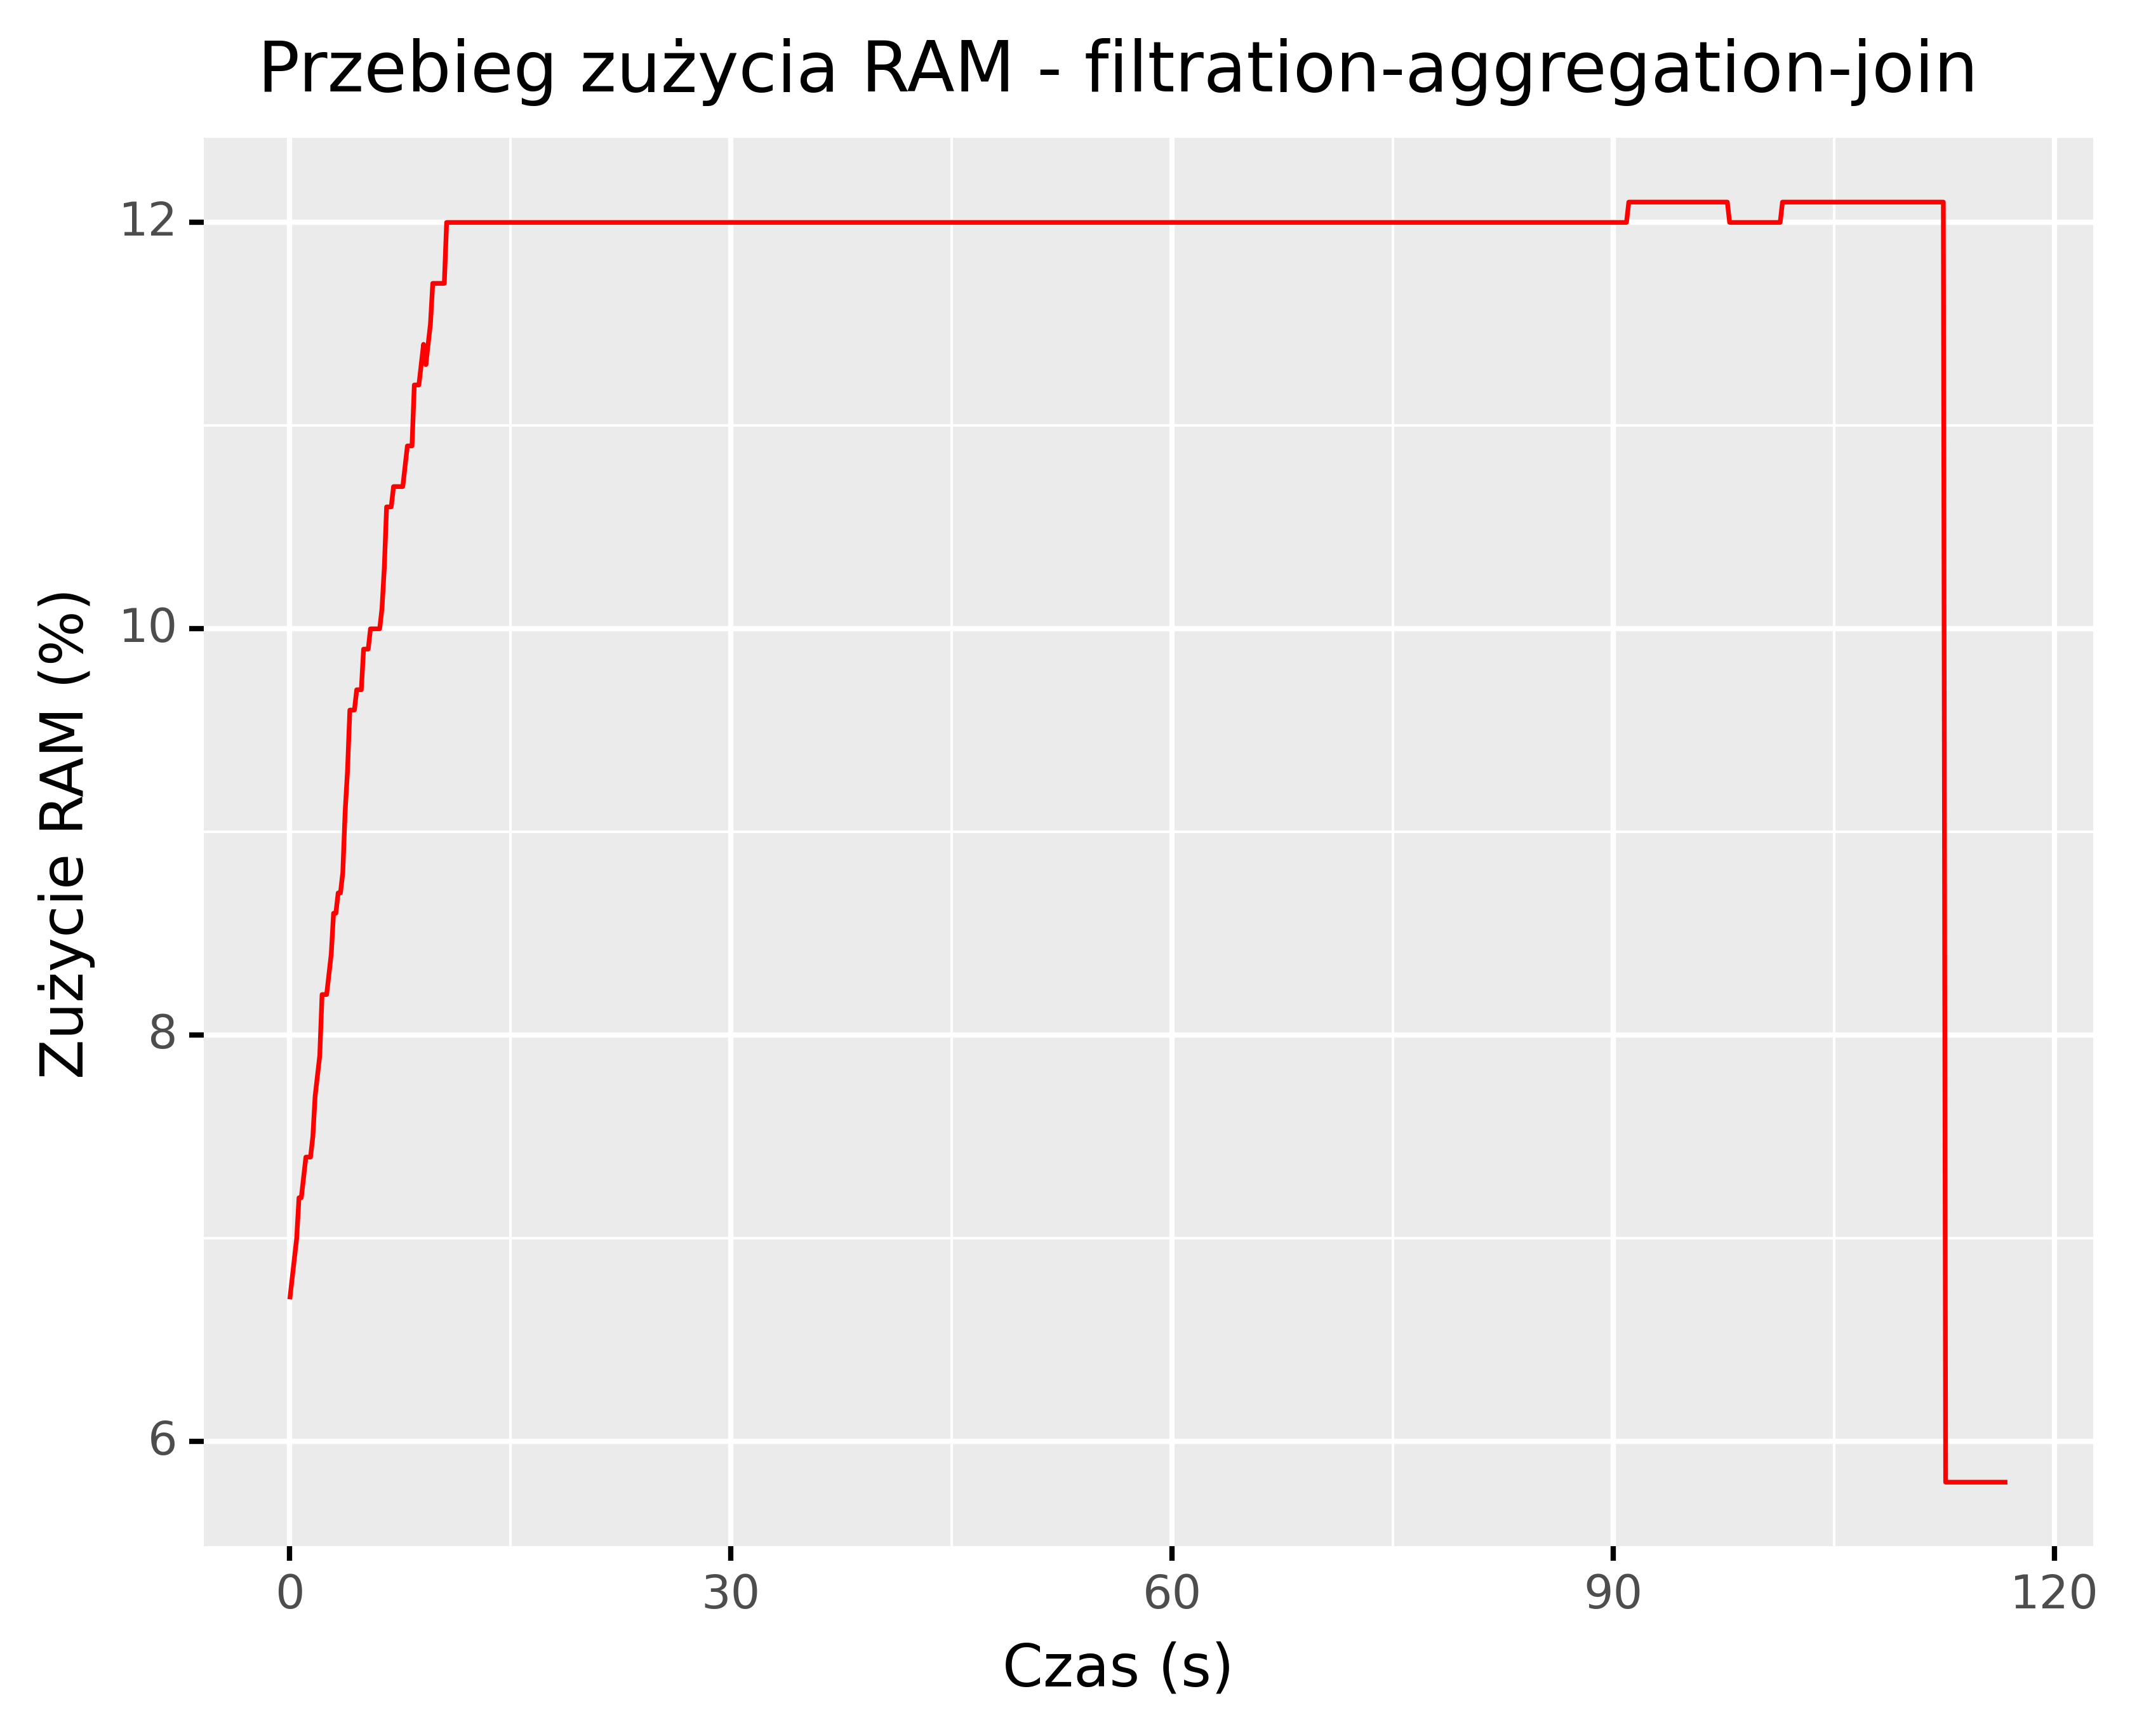
\includegraphics[width=0.5\textwidth]{figures/04-opis-danych/filtration-aggregation-join_example_ram_snapshot_1.png}\label{filtration-aggregation-join:f2}}
  \caption{Przykładowy przebieg zużycia zasobów dla filtracjo-agregacji z połączeniem (snapshot = 1)}
  \label{filtration-aggregation-join_example}
\end{figure}

\begin{figure}[!h]
  \centering
  \subfloat[CPU]{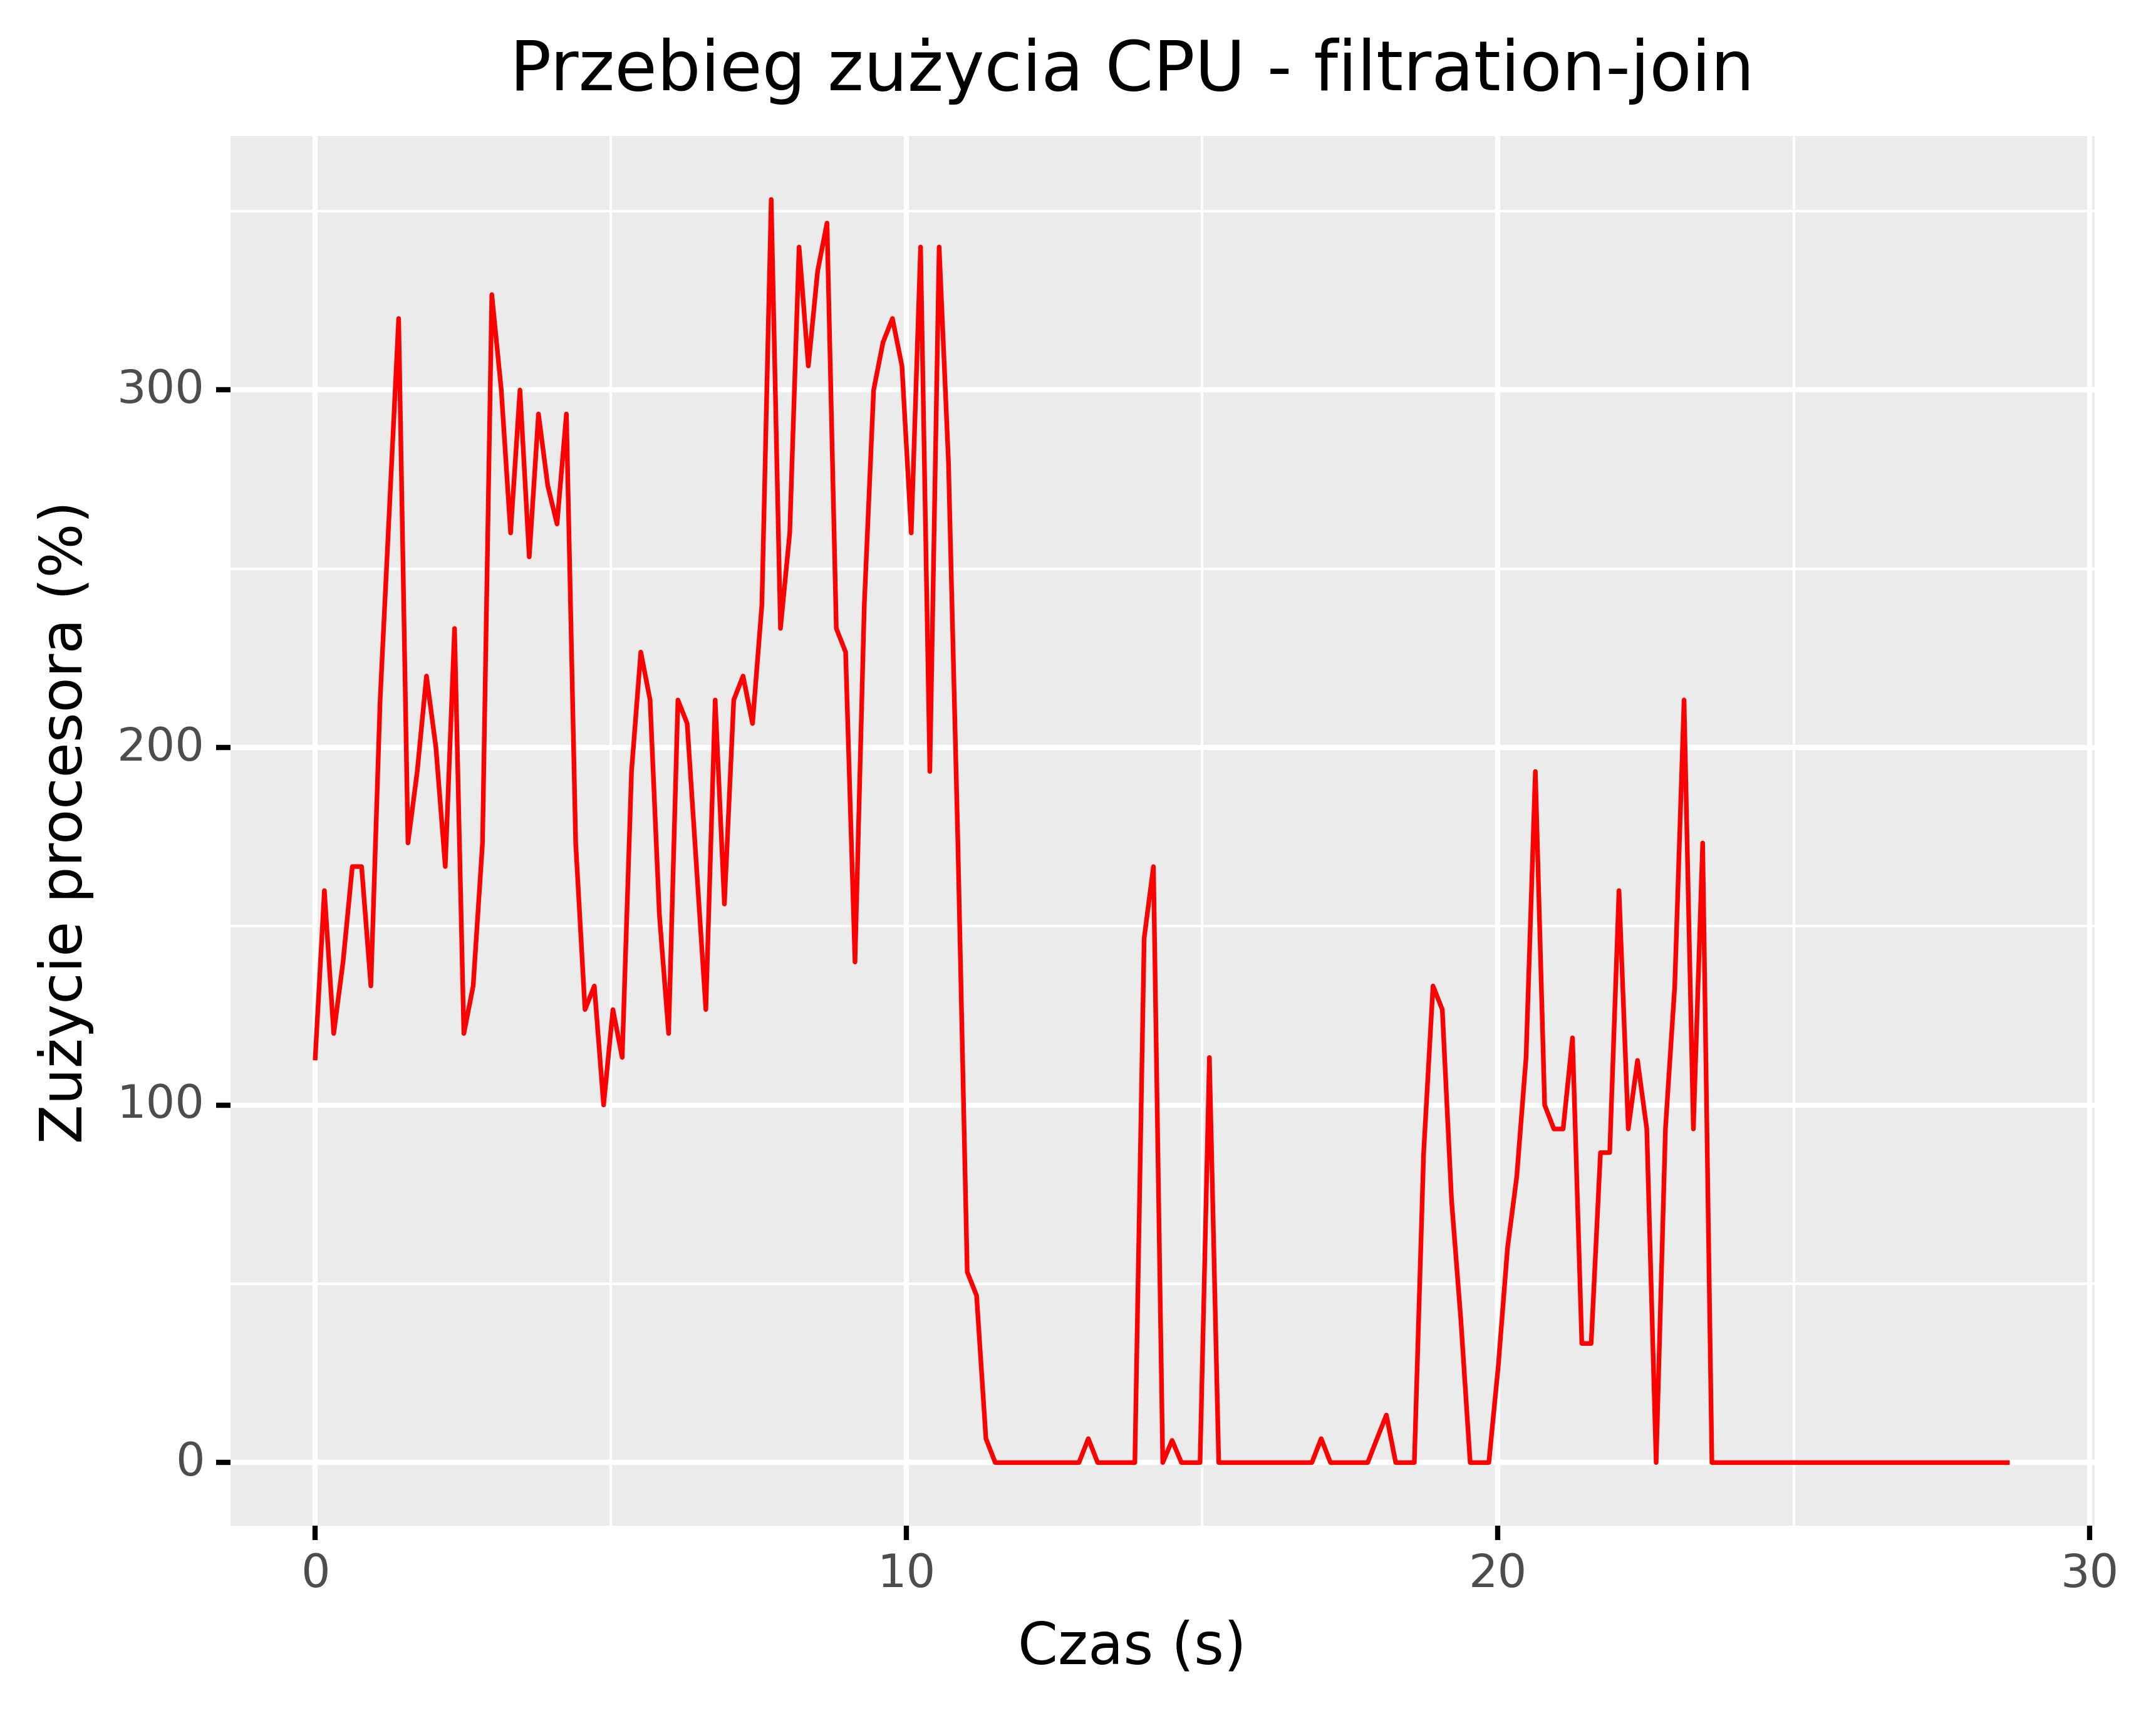
\includegraphics[width=0.5\textwidth]{figures/04-opis-danych/filtration-join_example_cpu_snapshot_1.png}\label{filtration-join_example:f1}}
  \hfill
  \subfloat[RAM]{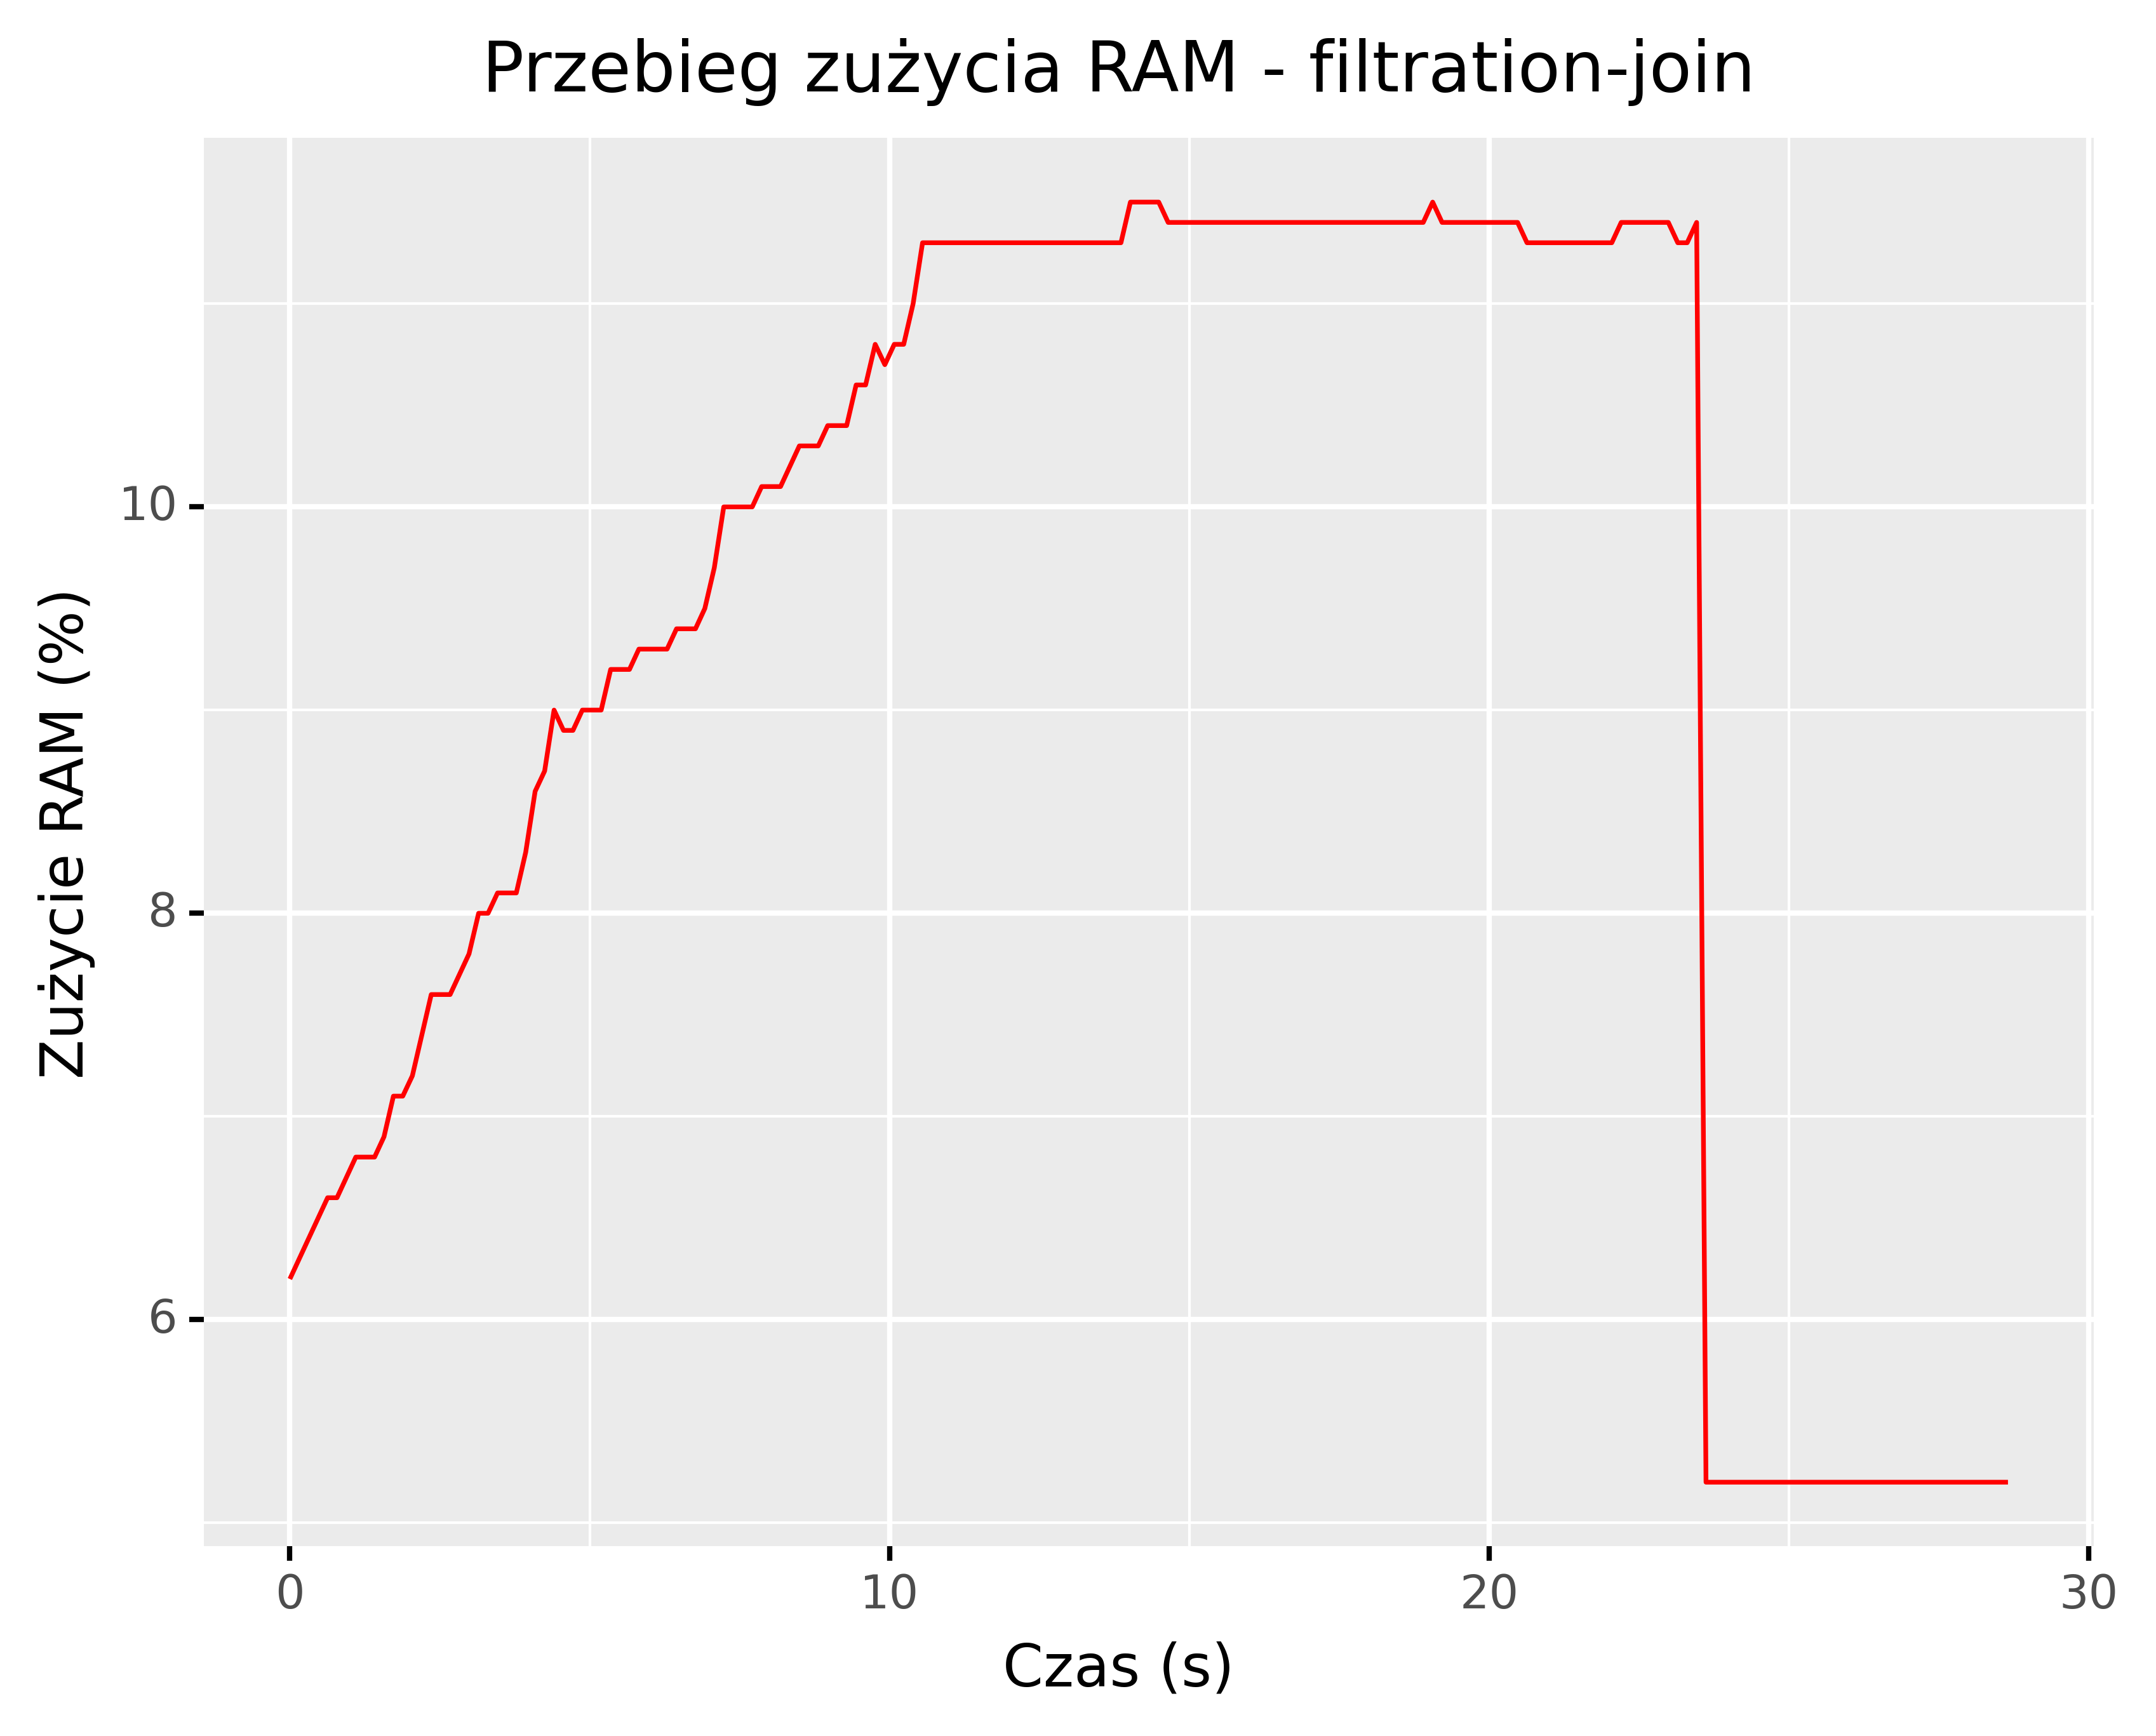
\includegraphics[width=0.5\textwidth]{figures/04-opis-danych/filtration-join_example_ram_snapshot_1.png}\label{filtration-join_example:f2}}
  \caption{Przykładowy przebieg zużycia zasobów dla filtracji z połączeniem (snapshot = 1)}
  \label{filtration-join_example}
  
\end{figure}

Na rysunkach \ref{aggregation_example} do \ref{filtration-join_example} widać, że wykresy CPU są bardzo ostre i mogły by zyskać na wygładzeniu krawędzi. Wykonaliśmy to przy użyciu średniej w oknie przesuwnym. Okno brało pod uwagę liczbę próbek zależną od tego jak dużo okno czasowe chcemy brać pod uwagę. Próbki są zebrane w odstępach 0.15 sekundy, więc ok sześciu próbek równe jest jednej sekundzie. Poniżej znajdują się wykresy przestawiający wygląd wykresów po wygładzeniu dla różnej liczby próbek dla przykładowego przebiegu agregacji.

\begin{figure}[H]
  \centering
  \subfloat[CPU]{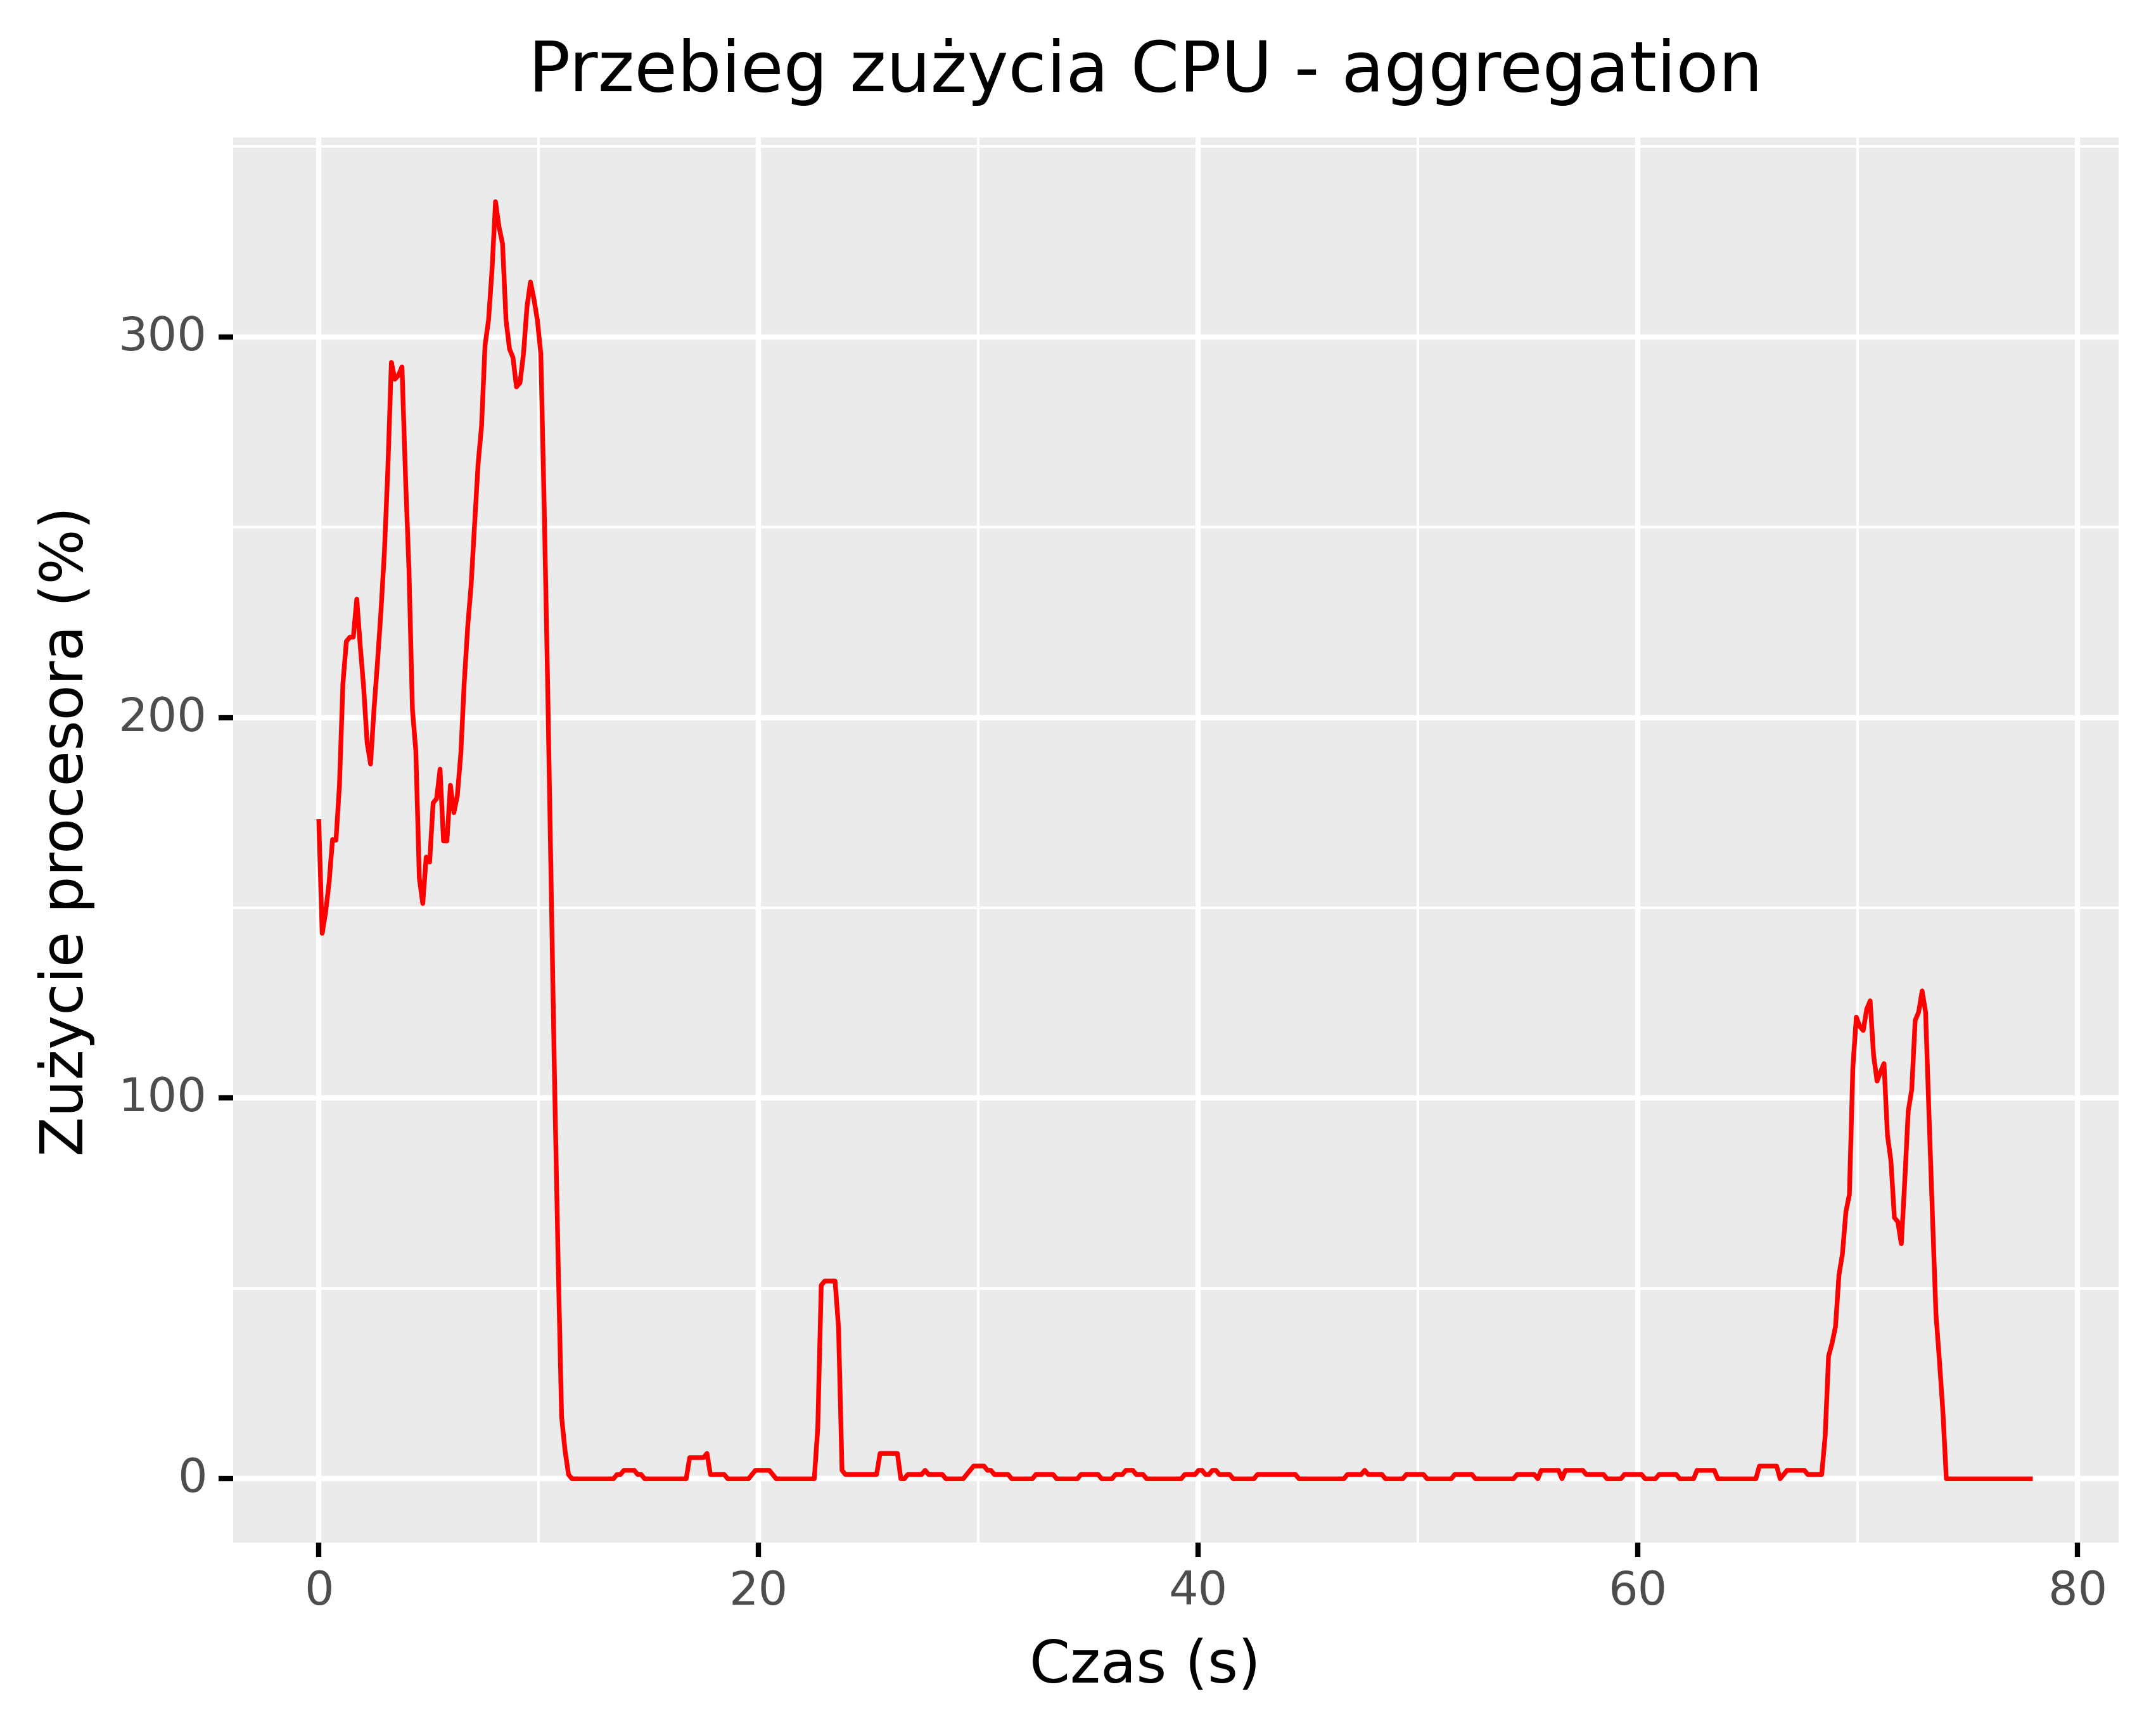
\includegraphics[width=0.5\textwidth]{figures/04-opis-danych/aggregation_smooth_6_cpu_snapshot_1.png}\label{aggregation_smooth_6:f1}}
  \hfill
  \subfloat[RAM]{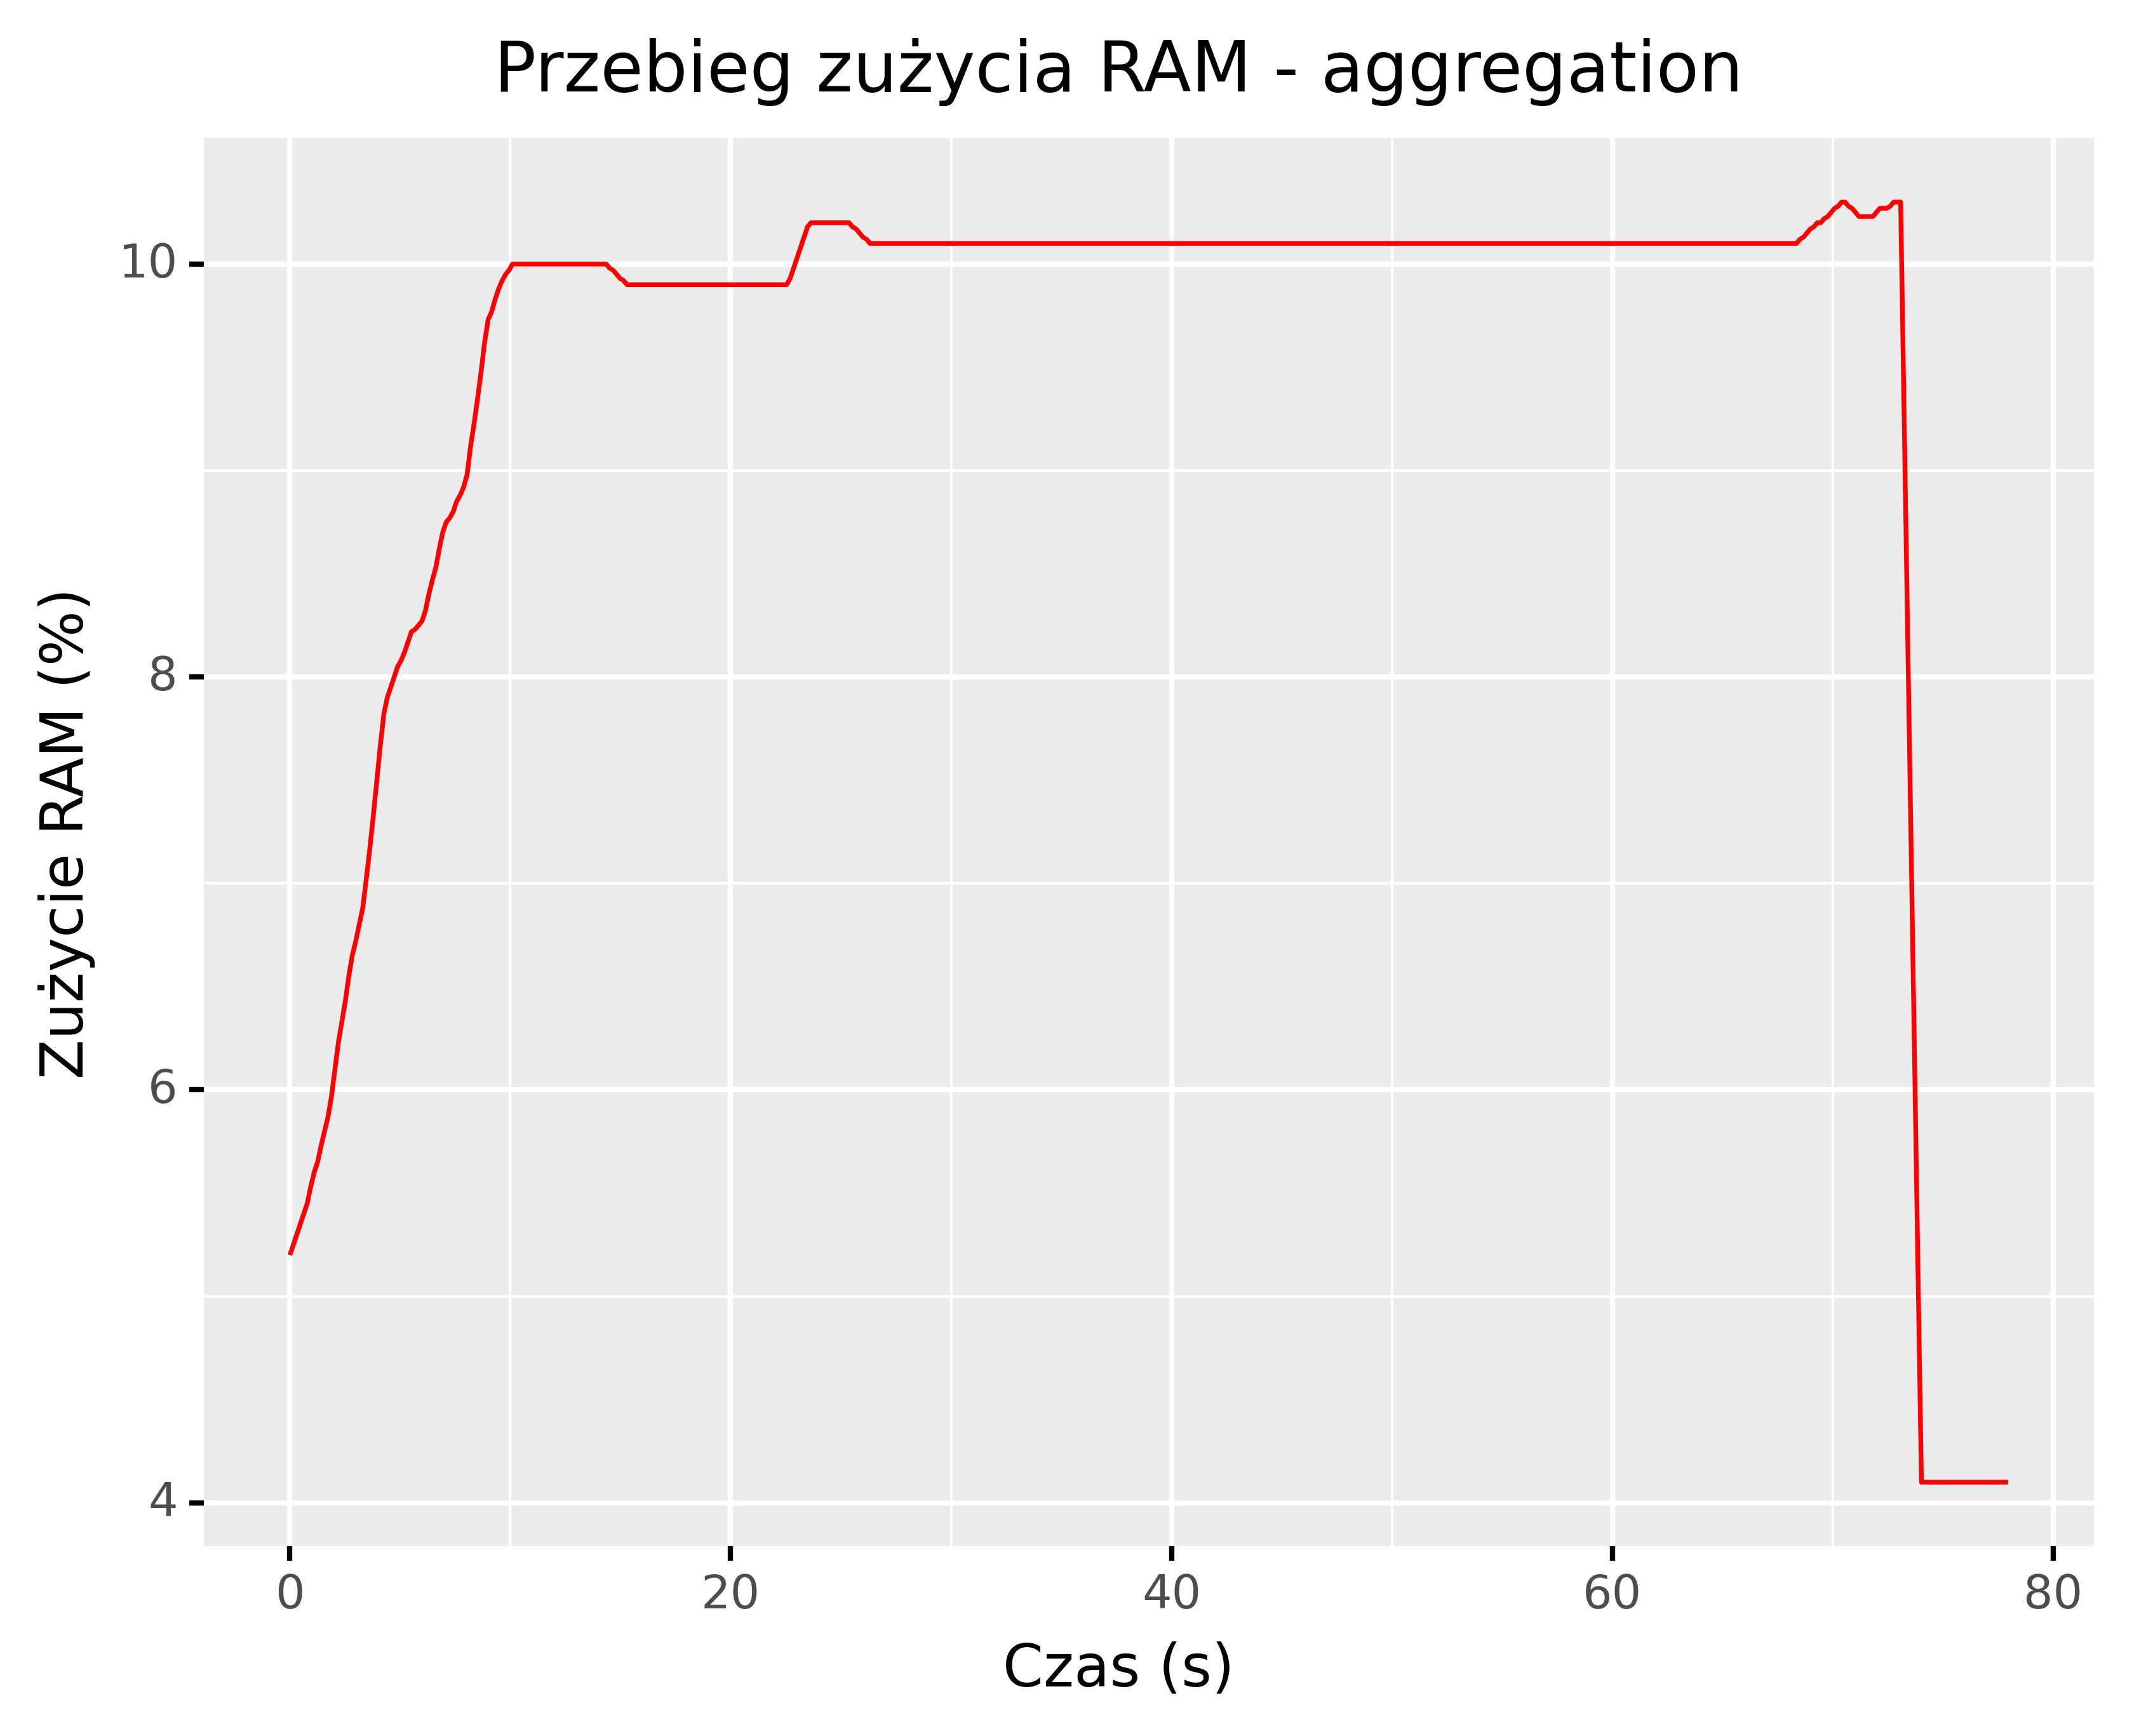
\includegraphics[width=0.5\textwidth]{figures/04-opis-danych/aggregation_smooth_6_ram_snapshot_1.png}\label{aggregation_smooth_6:f2}}
  \caption{Przykładowy wygładzony wykres zużycia zasobów dla agregacji (snapshot = 1, okno 1 sekundowe)}
  \label{aggregation_smooth_6}
\end{figure}

\begin{figure}[H]
  \centering
  \subfloat[CPU]{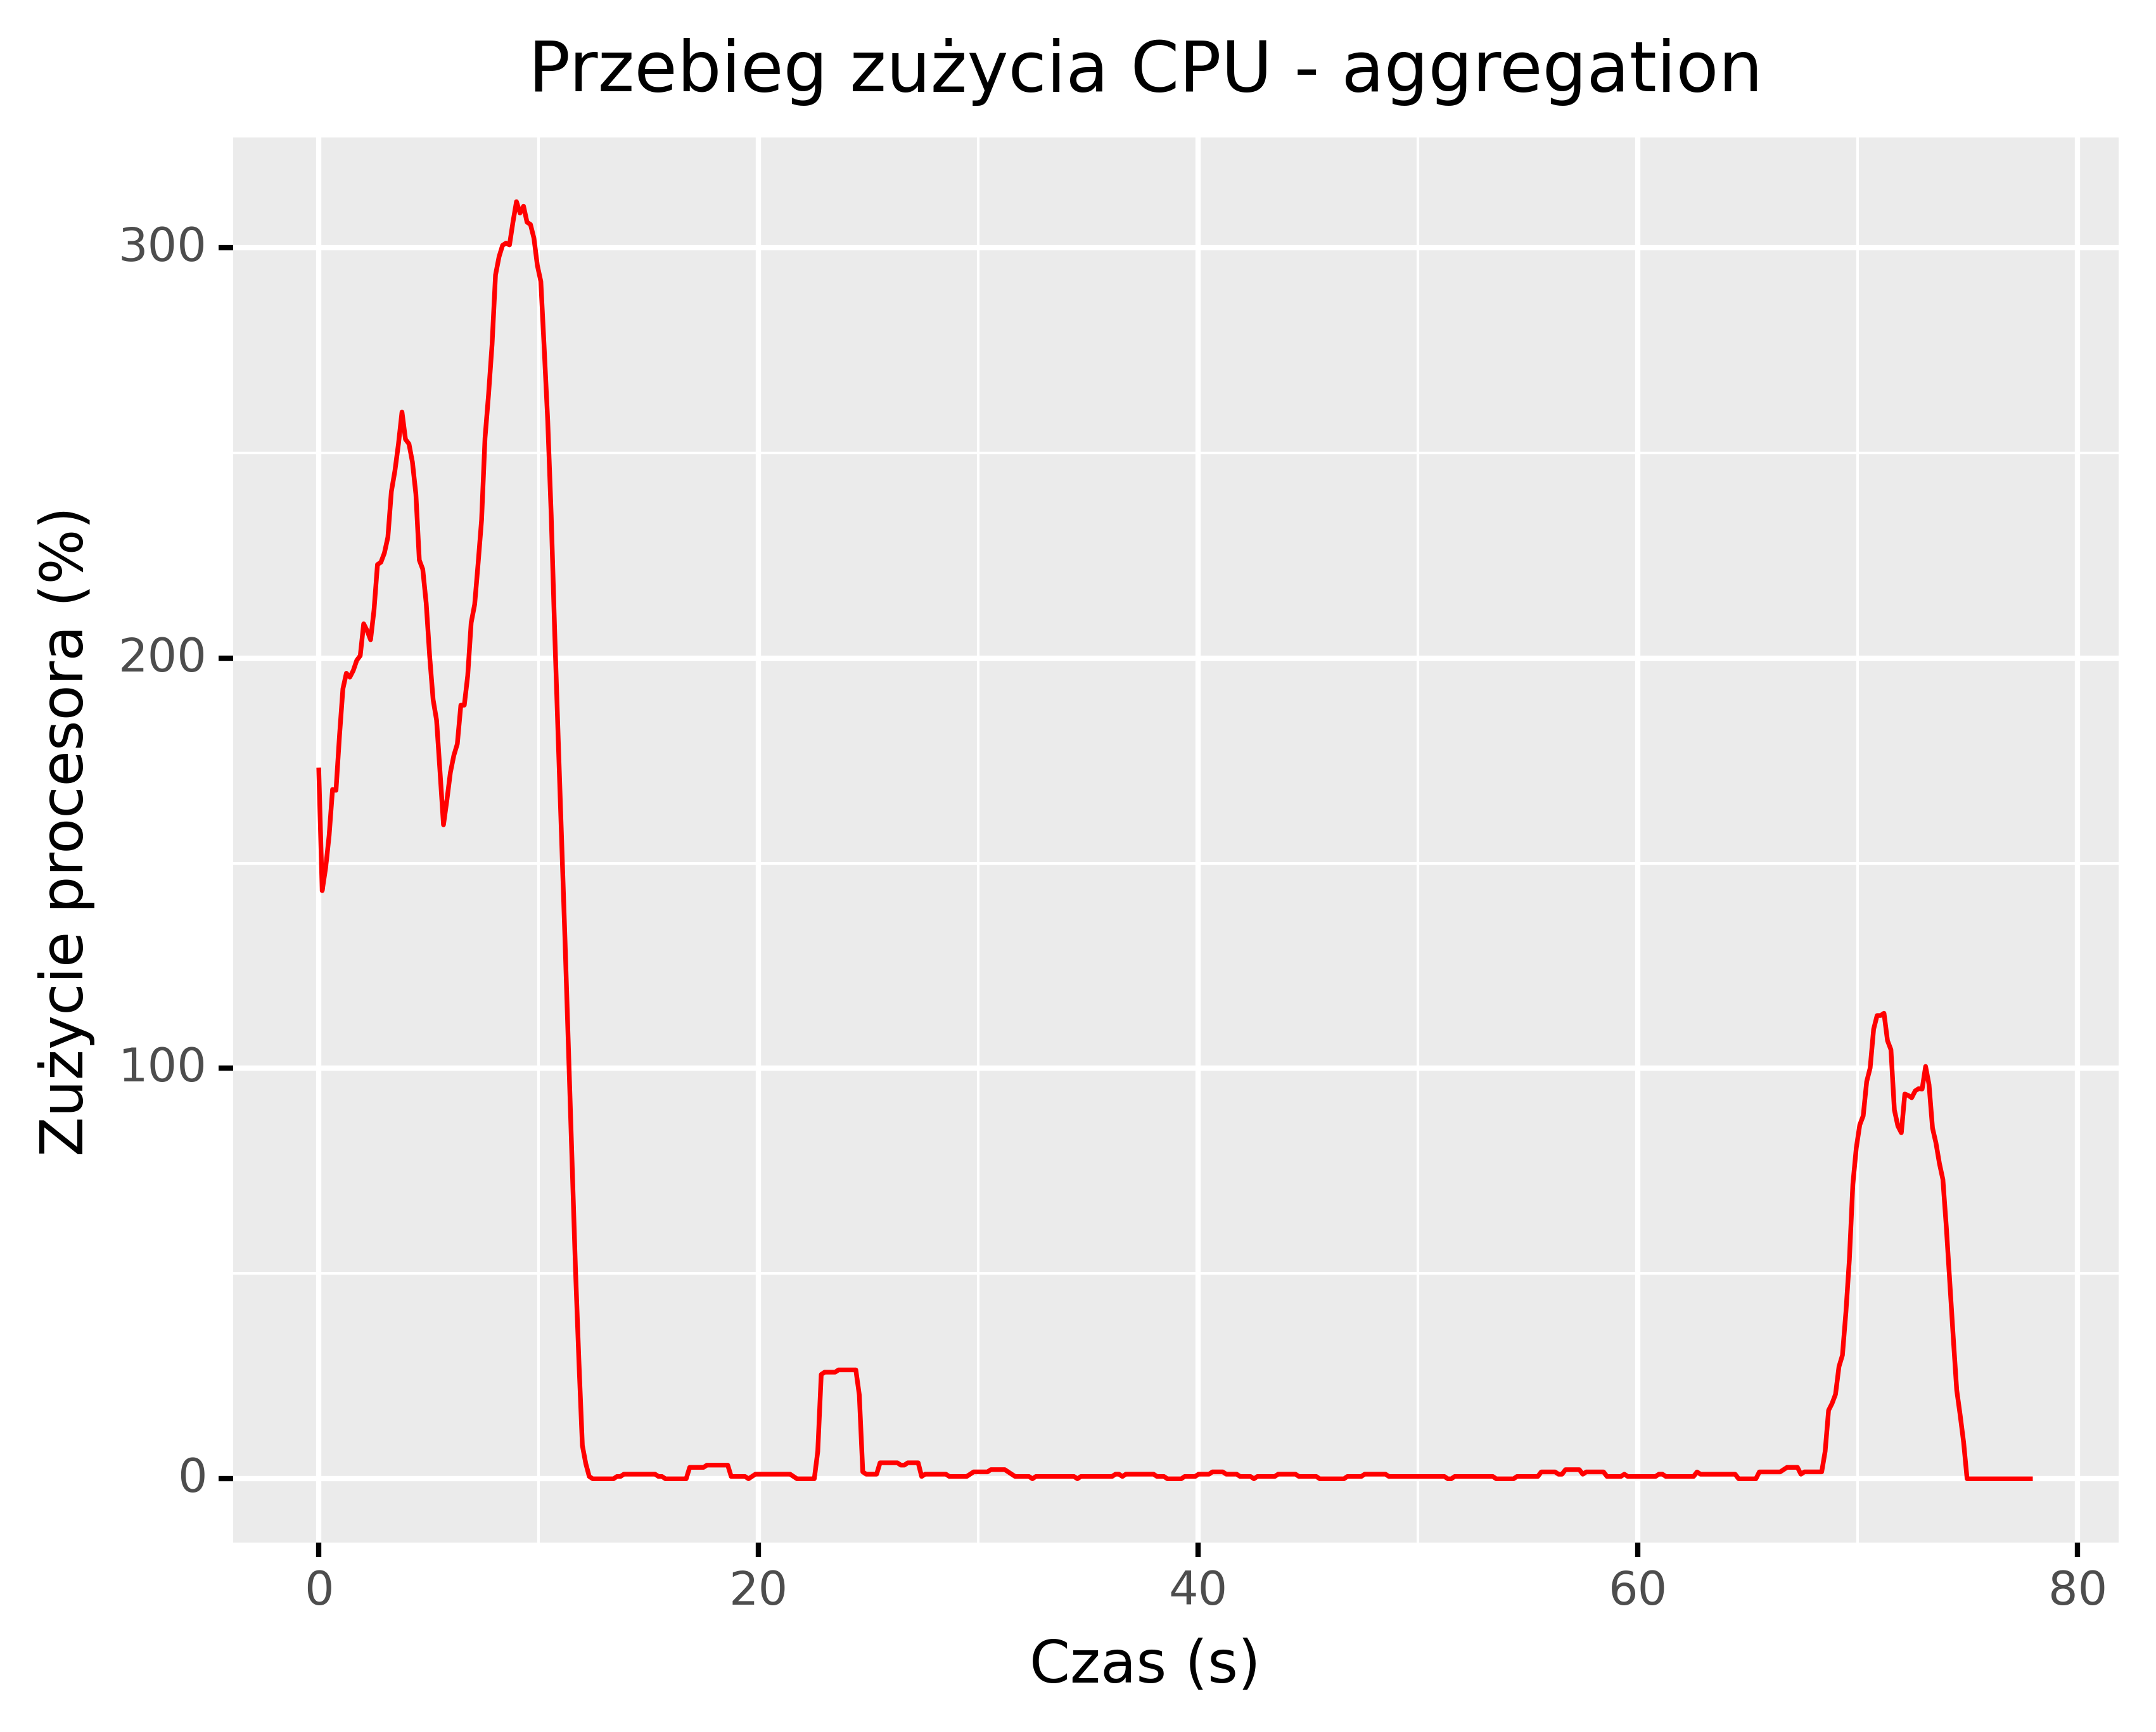
\includegraphics[width=0.5\textwidth]{figures/04-opis-danych/aggregation_smooth_12_cpu_snapshot_1.png}\label{aggregation_smooth_12:f1}}
  \hfill
  \subfloat[RAM]{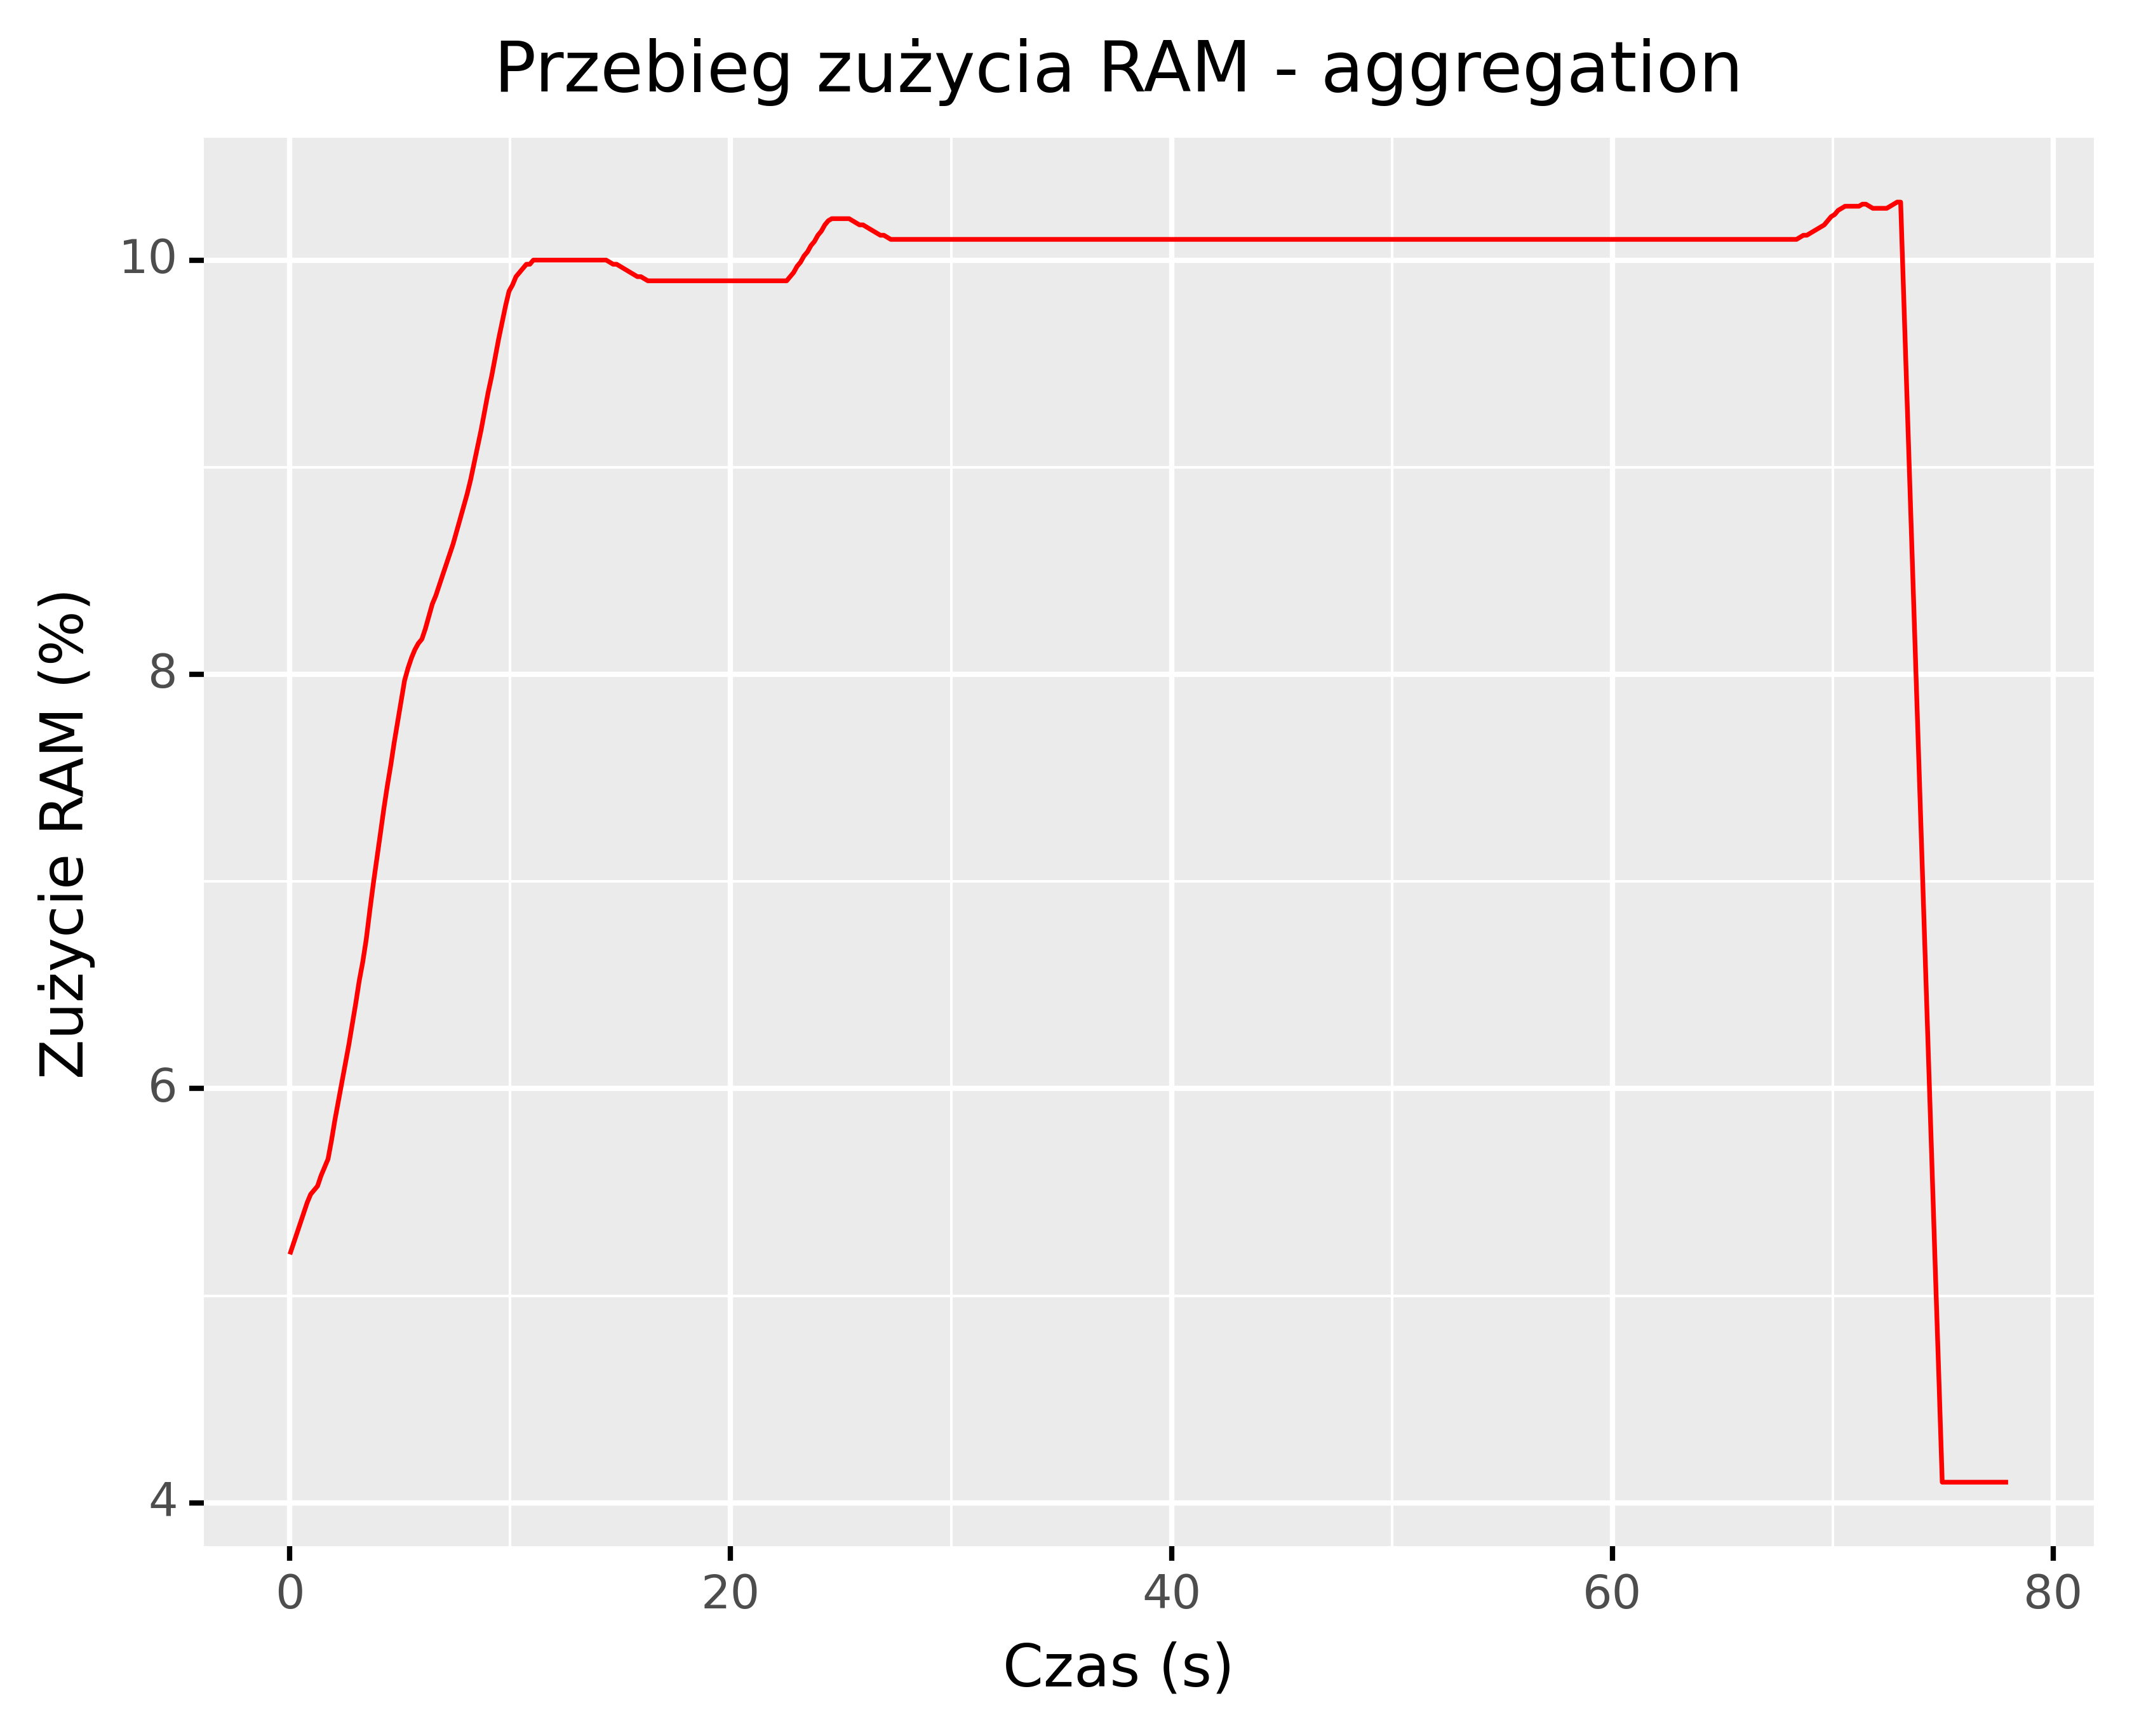
\includegraphics[width=0.5\textwidth]{figures/04-opis-danych/aggregation_smooth_12_ram_snapshot_1.png}\label{aggregation_smooth_12:f2}}
  \caption{Przykładowy wygładzony wykres zużycia zasobów dla agregacji (snapshot = 1, okno 2 sekundowe)}
  \label{aggregation_smooth_12}
\end{figure}

\begin{figure}[H]
  \centering
  \subfloat[CPU]{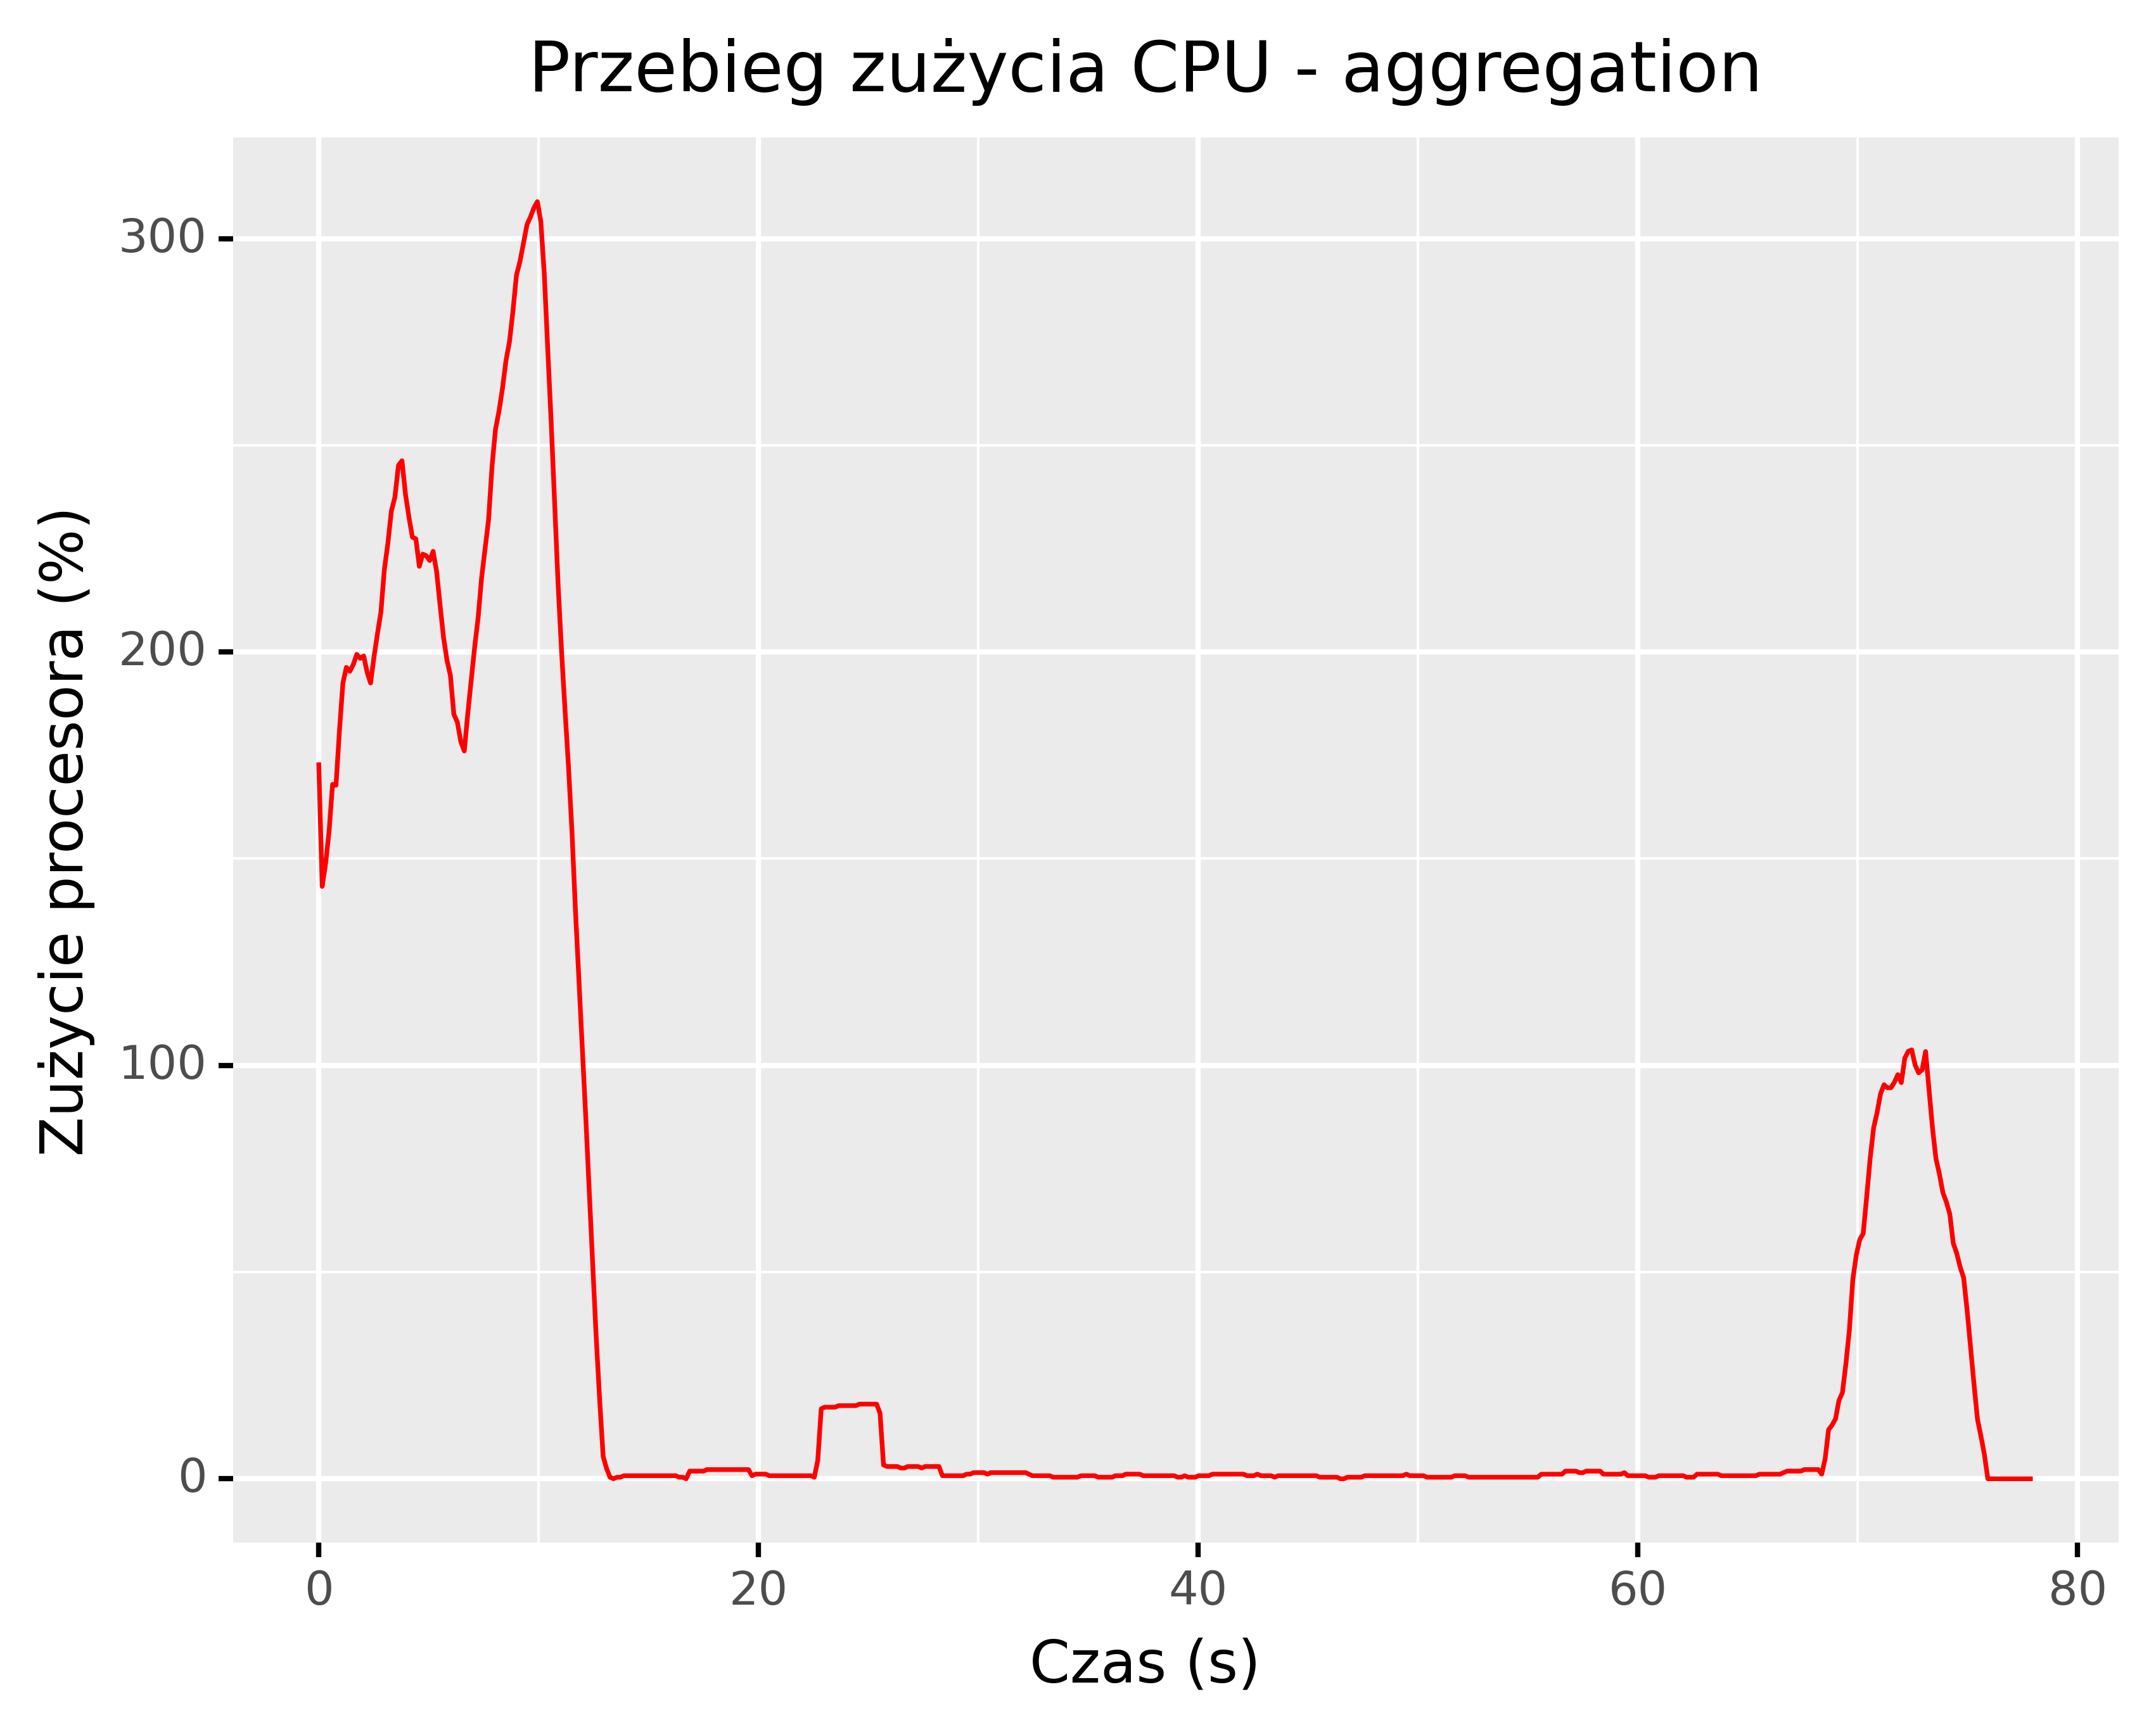
\includegraphics[width=0.5\textwidth]{figures/04-opis-danych/aggregation_smooth_18_cpu_snapshot_1.png}\label{aggregation_smooth_18:f1}}
  \hfill
  \subfloat[RAM]{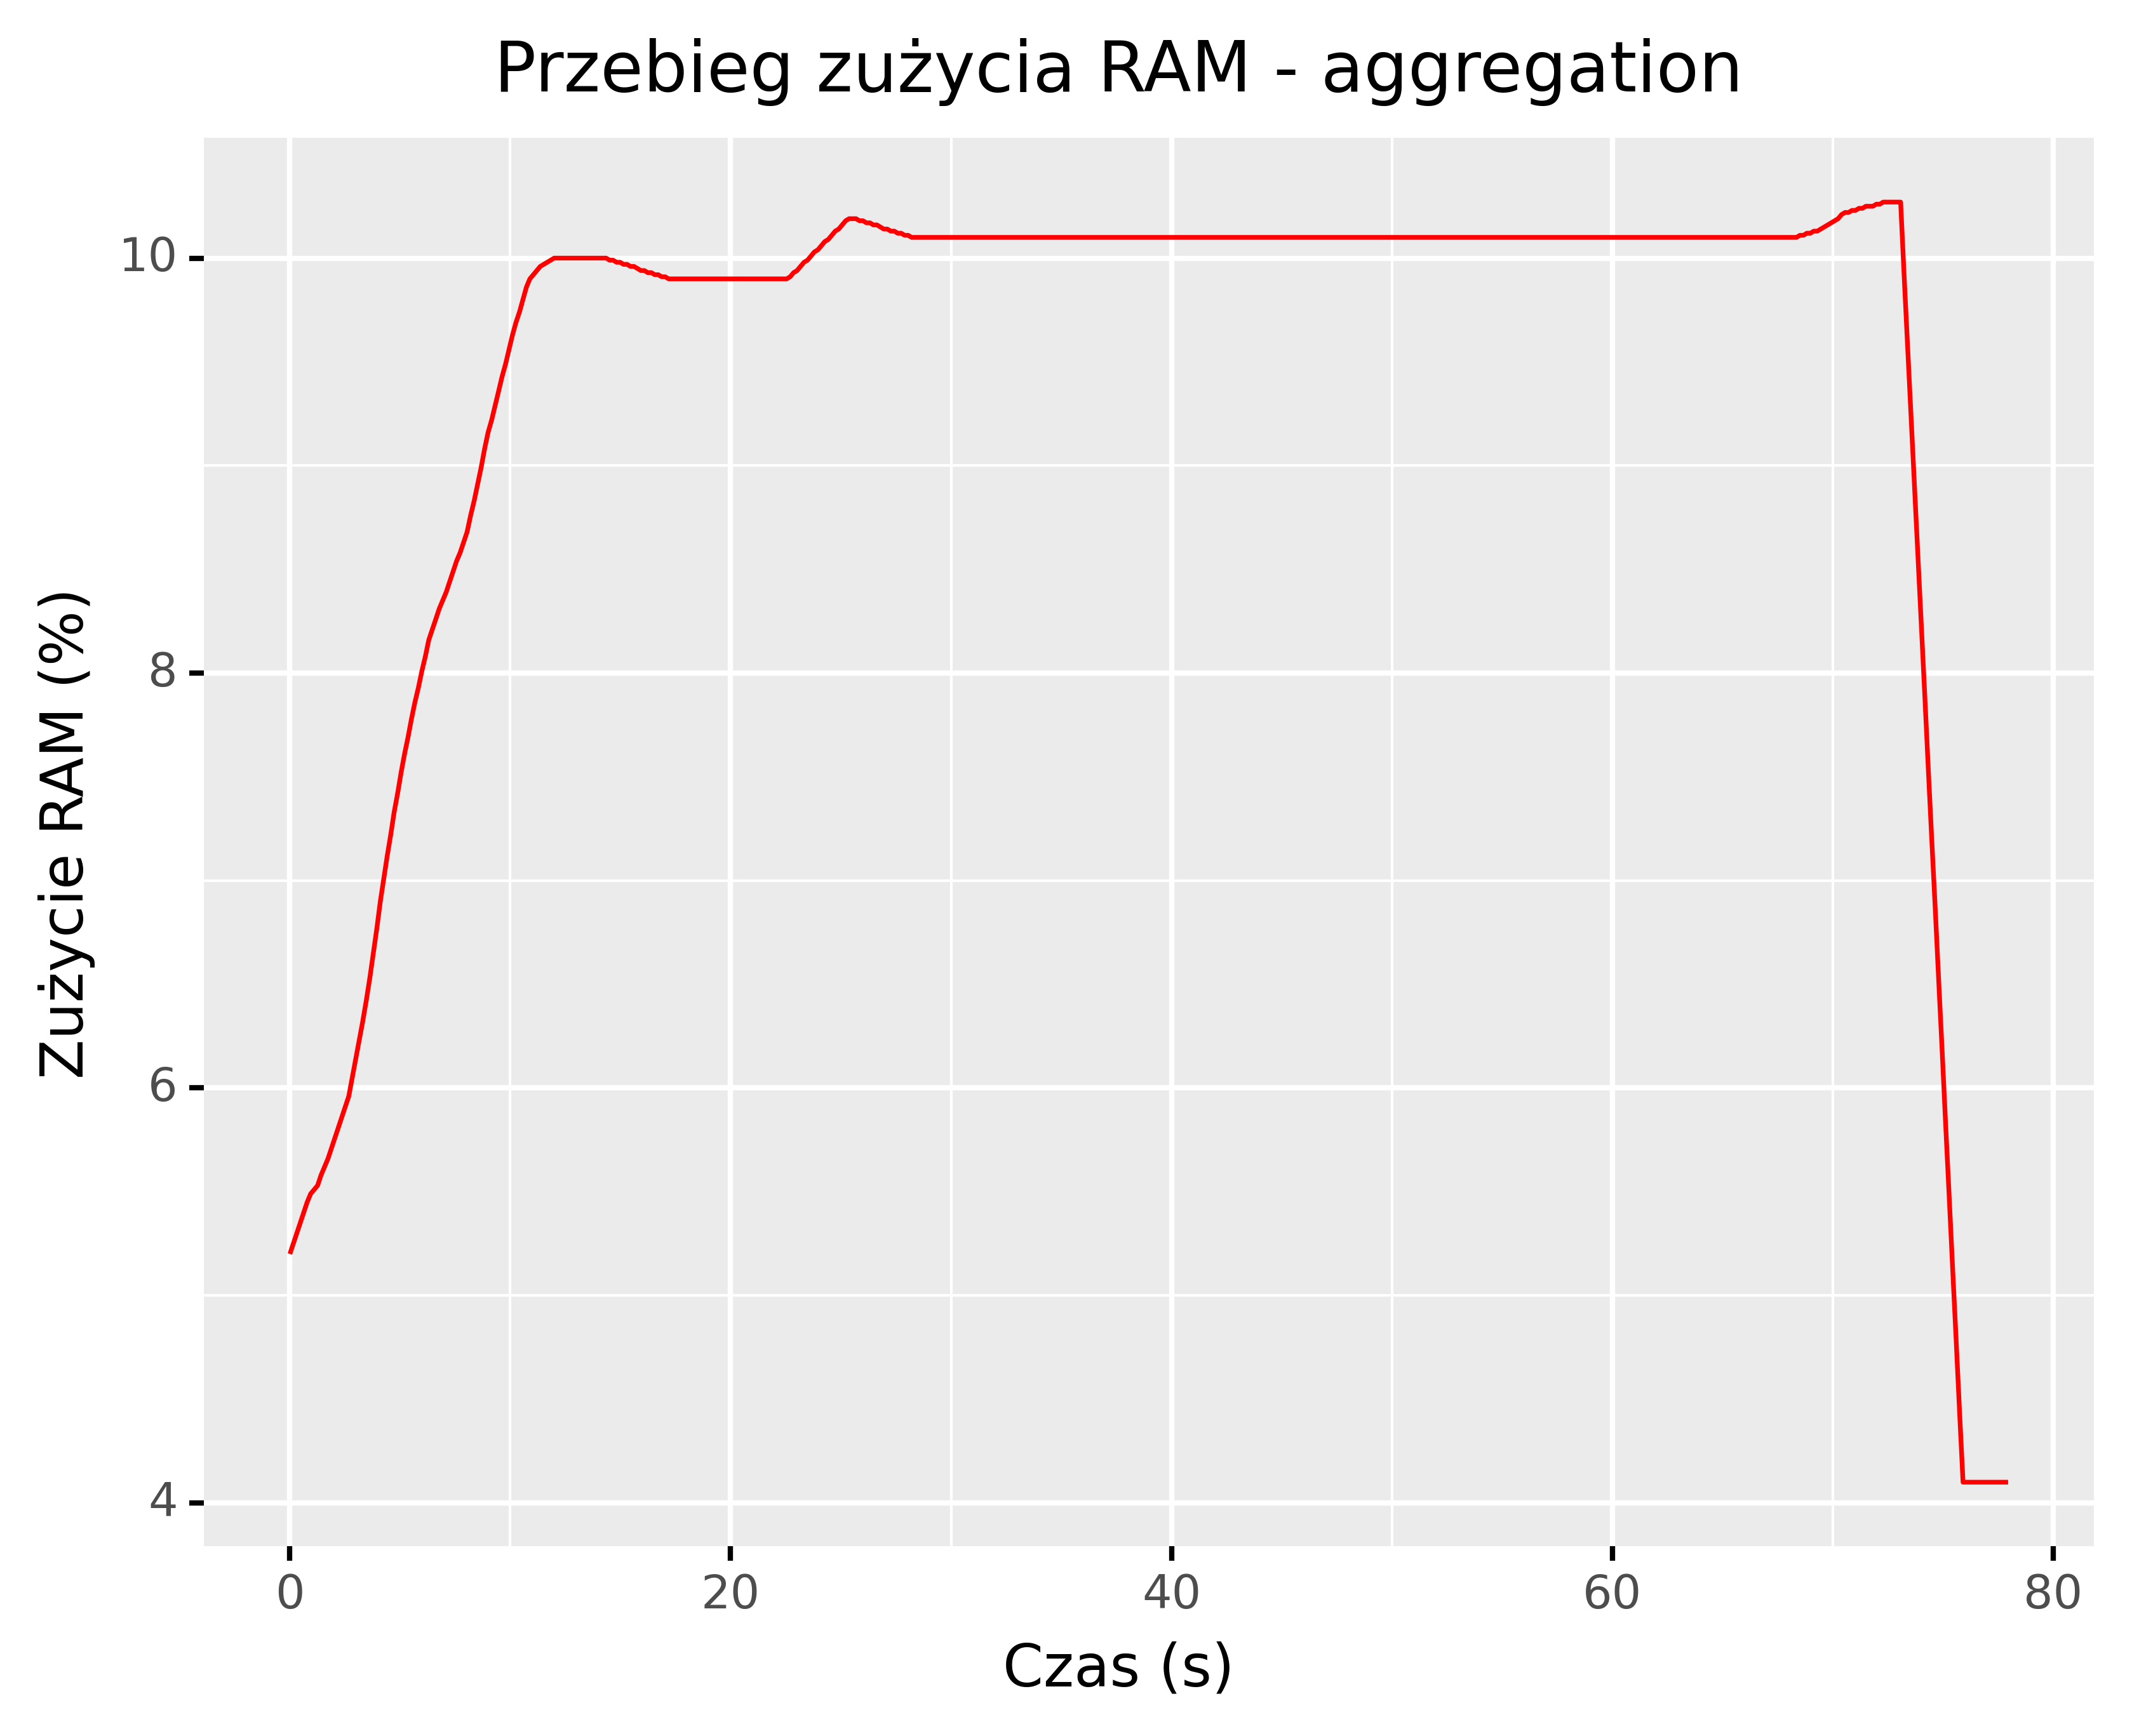
\includegraphics[width=0.5\textwidth]{figures/04-opis-danych/aggregation_smooth_18_ram_snapshot_1.png}\label{aggregation_smooth_18:f2}}
  \caption{Przykładowy wygładzony wykres zużycia zasobów dla agregacji (snapshot = 1, okno 3 sekundowe)}
  \label{aggregation_smooth_18}
\end{figure}

Po wykonaniu transformacji można zauważyć, że wykresy są mniej niestabilne (mniej dużej ilości skoków wartości w małym przedziale czasowym). Rysunki od \ref{aggregation_smooth_6} do \ref{aggregation_smooth_18} pokazują na przykładzie agregacji wyniki dla kolejno 6, 12 i 18 próbek (czyli 1, 2, 3 sekundy). Ostatecznie nie chcąc przesadzić będziemy korzystali prawdopodobnie z oknem 1 sekundowym, żeby nie stracić zbyt wielu informacji, co mogłoby się zdarzyć używając zbyt dużego okna. Przykładowo na rysunku CPU \ref{aggregation_smooth_18} widać w porównaniu z rysunkiem \ref{aggregation_smooth_6} mocno zmniejszony szczyt w okolicy 25 sekundy.

Ostatnią transformacją przeprowadzoną na danych wejściowych jest standaryzacja danych. Wykonana jest ona w celu sprawdzenia czy wybrane algorytmy liczenia podobieństwa między szeregami lepiej poradzą sobie z danymi niezmienionymi, czy jednak ustandaryzowanymi. Metoda użyta w naszym przetwarzaniu wykorzystuje średnie wartości oraz odchylenie standardowe w ramach jednego szeregu dla poszczególnych cech (CPU, RAM). Wpierw od każdej wartości odejmujemy średnią, a następnie wynik dzielimy przez odchylenie standardowe.

\begin{figure}[H]
  \centering
  \subfloat[CPU]{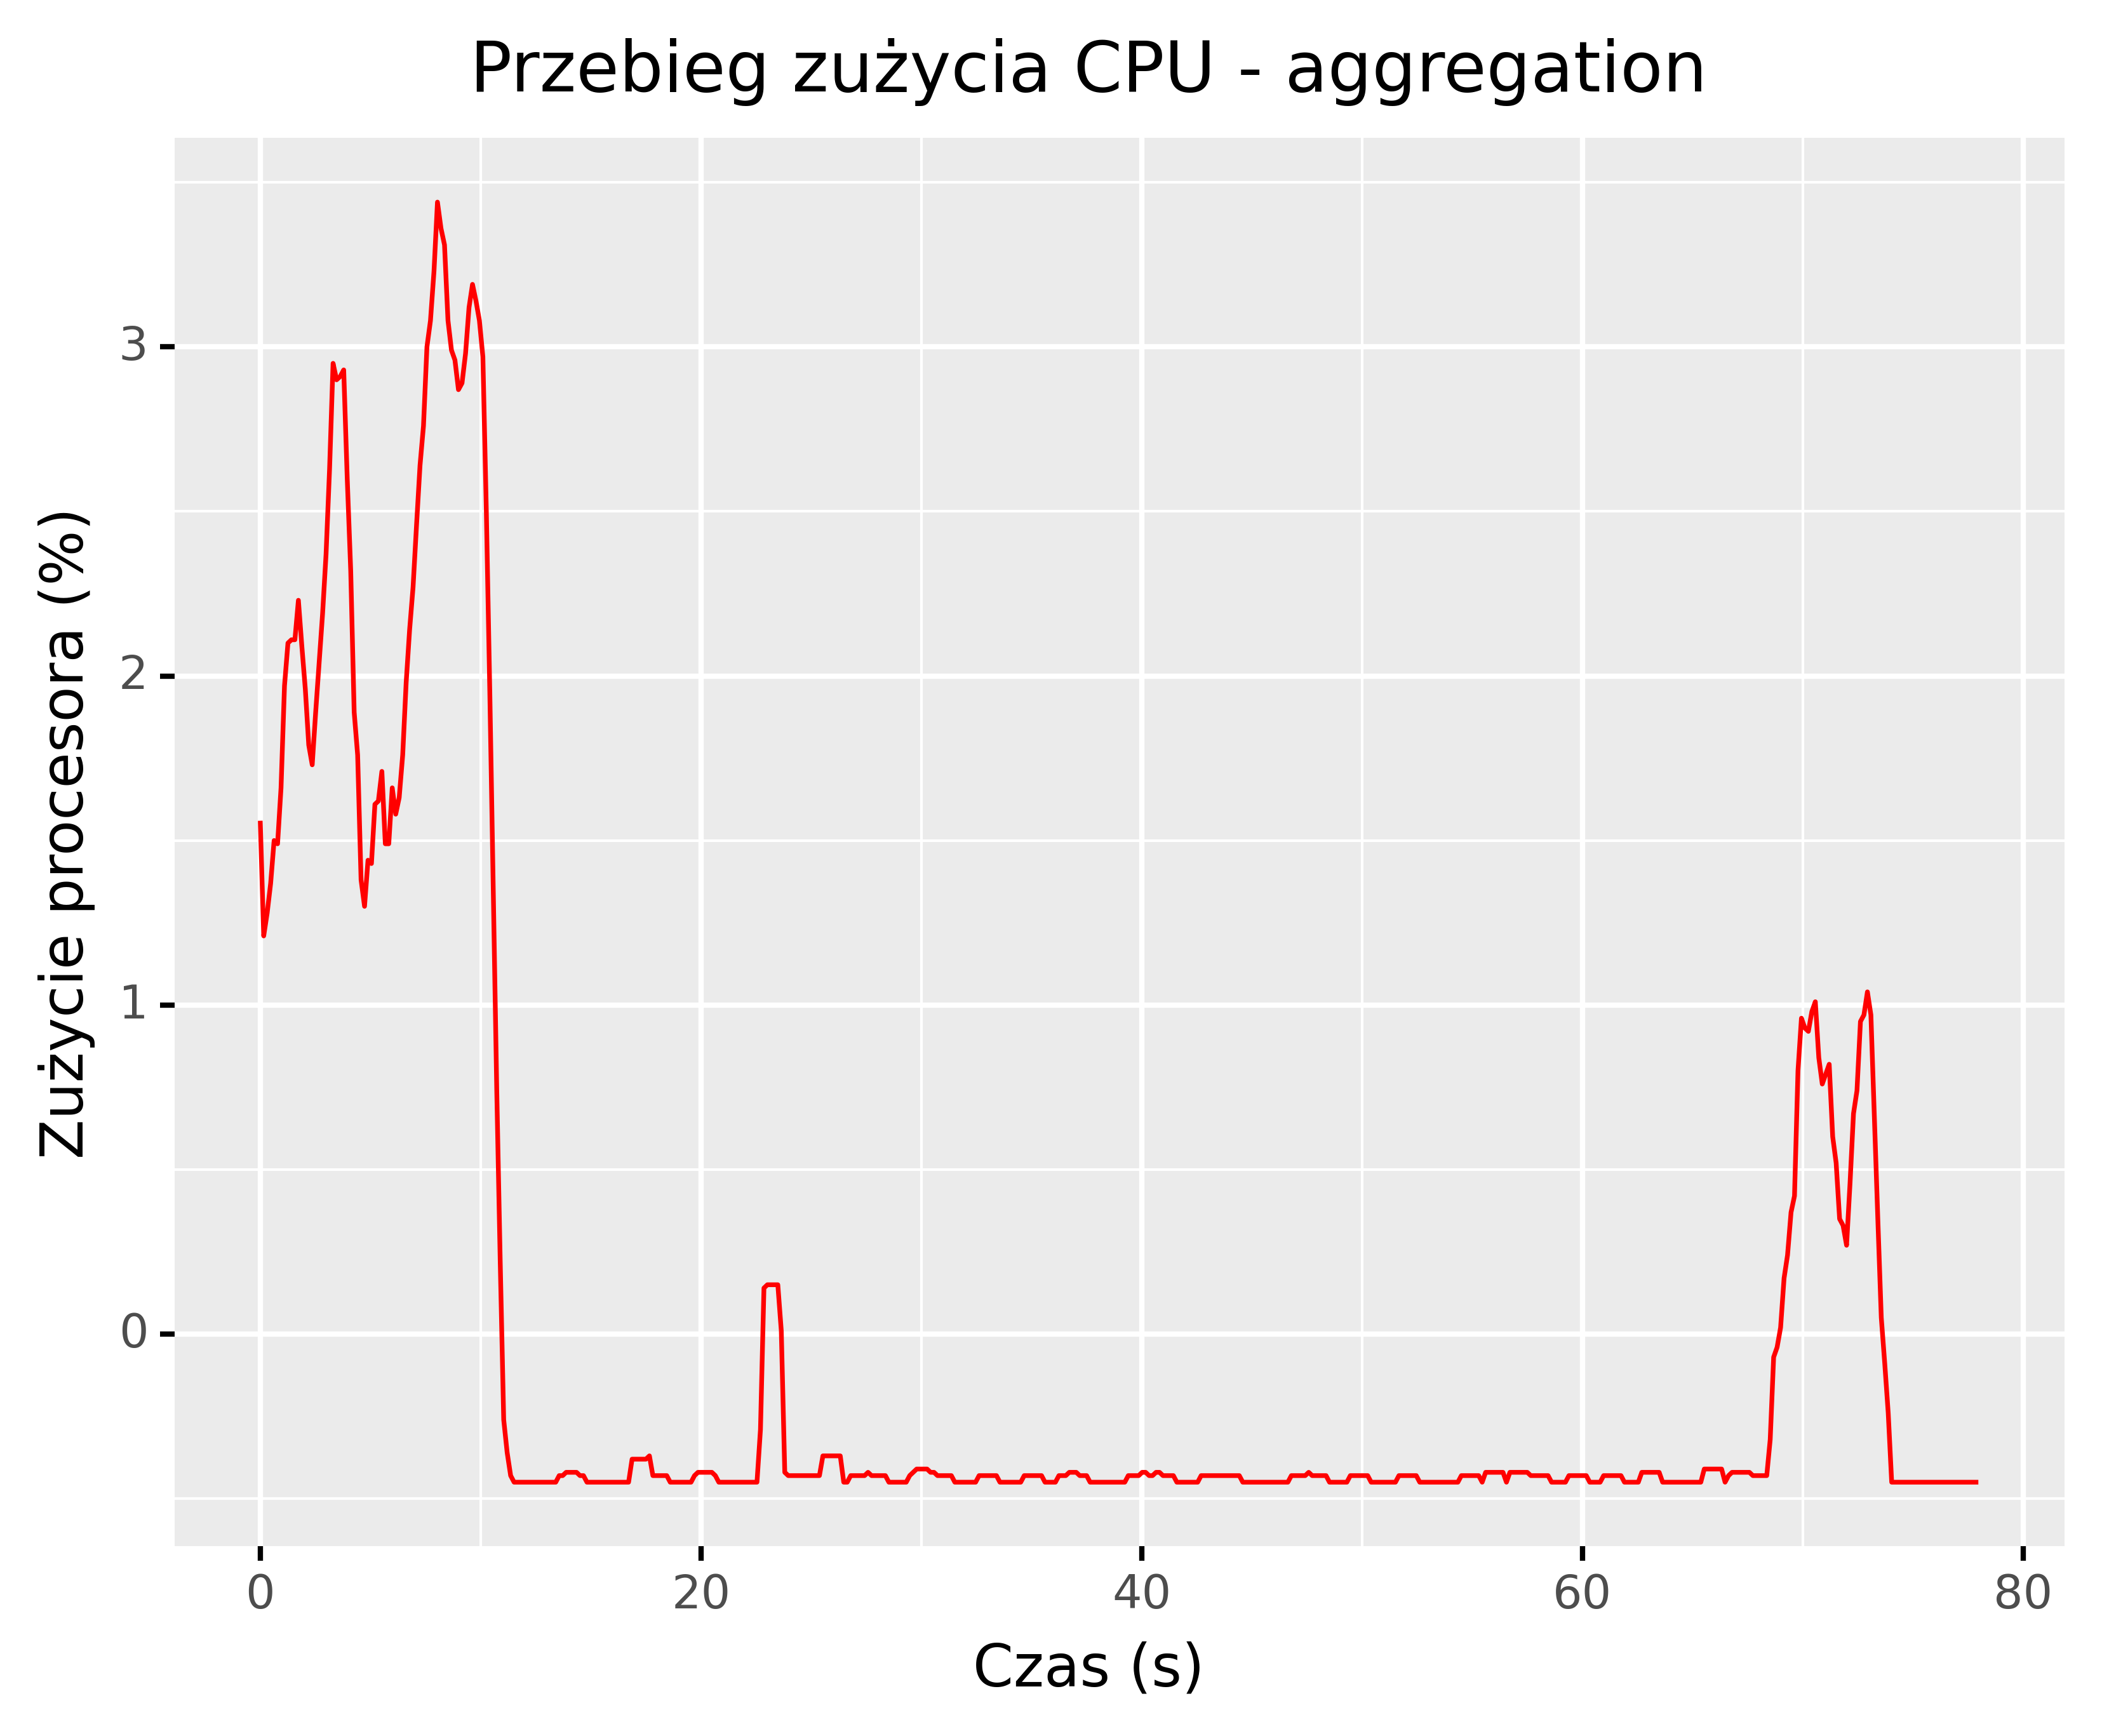
\includegraphics[width=0.5\textwidth]{figures/04-opis-danych/aggregation_smooth_standardised_cpu_snapshot_1.png}\label{aggregation_standardised:cpu}}
  \hfill
  \subfloat[RAM]{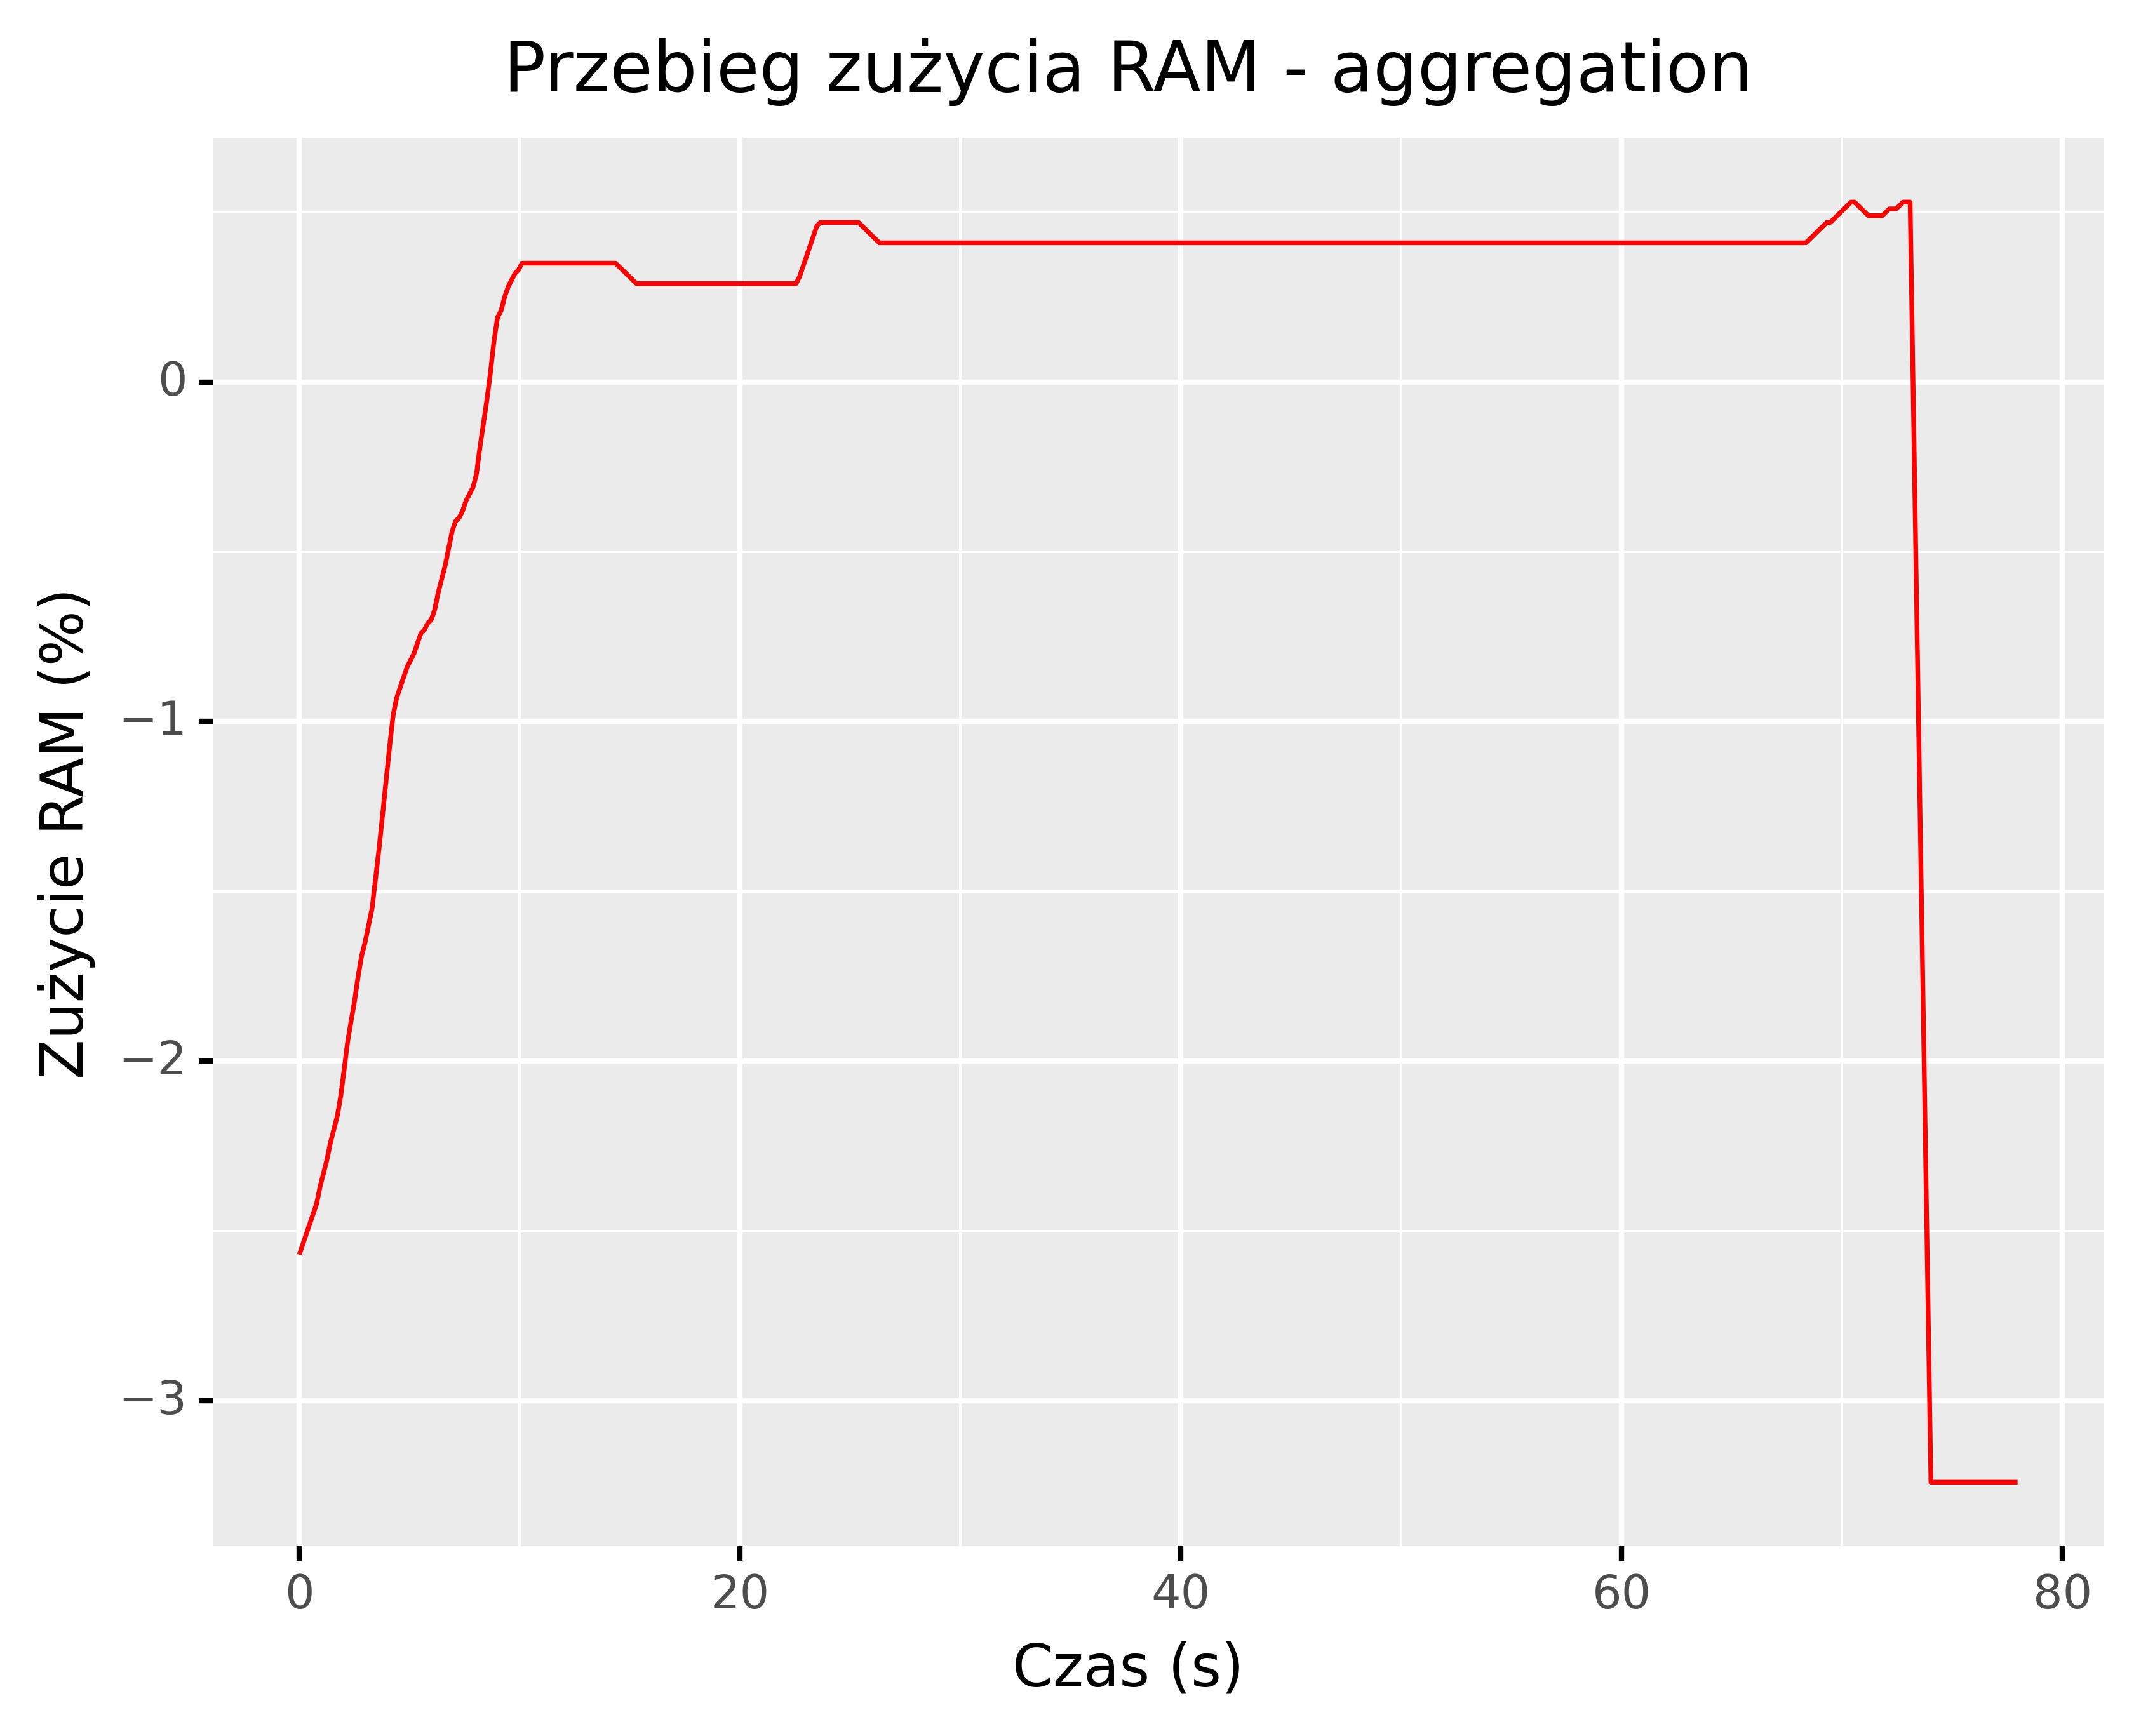
\includegraphics[width=0.5\textwidth]{figures/04-opis-danych/aggregation_smooth_standardised_ram_snapshot_1.png}\label{aggregation_standardised:ram}}
  \caption{Przykładowy ustandaryzowany wykres zużycia zasobów dla agregacji (snapshot = 1))}
  \label{aggregation_standardised}
\end{figure}

Na wykresach \ref{aggregation_standardised} widać że po wykonaniu standaryzacji kształt wykresów się nie zmienił (porównując z \ref{aggregation_smooth_6}), jednak amplitudy zmalały. W ten sposób przygotowane dane zostaną wykorzystane w eksperymentach, sprawdzając ich skuteczność przed i po standaryzacji.

\section{Charakterystyka danych wejściowych}
\begin{itemize}
    \item usunięcie identyfikatorów procesów
    \item zgrupowanie względem znacznika czasowego i zsumowanie
    \item analiza danych od około 50 próbki
\end{itemize}
\section{Cechy danych w kontekście wyboru algorytmu}
\subsection{Porównanie próbek o tych samych parametrach}
\begin{itemize}
    \item mogą się zdarzyć wartości odstające - z czym średnio radzi sobie odległość Euklidesowa
\end{itemize}
\subsection{Wpływ zmiany rozmiaru danych na uzyskany przebieg:}\begin{itemize}
    \item skalowanie amplitudy i skalowanie czasu
    \item DTW radzi sobie ze skalowaniem czasu, ale nie ze skalowaniem amplitudy. W tym wypadku prawdopodobnie lepiej zadziała Landmark Similarity
\end{itemize}

\subsection{Wpływ zmiany konfiguracji klastra (liczby węzłów roboczych) na uzyskany przebieg:}
\begin{itemize}
    \item brak większego wpływu - nie widać wpływu liczby węzłów na amplitudę lub czas
    \item skoro brak wpływu to można wykorzystać amplitudę do liczenia podobieństwa: DTW
    \item skoro brak wpływu na czas to odległość Euklidesowa również powinna być odpowiednia
    \item Sam Landmark Similarity nie wykorzystywałby informacji o amplitudzie i podobnym czasie 
\end{itemize}

\section{Wyniki eksperymentów}
Wykorzystane implementacje algorytmów:
\begin{itemize}
    \item scipy.spatial - distance.euclidean()
    \item dtw-python - distance(), normalizeDistance()
    \item dtaidistance - distance()
\end{itemize}
\subsection{dtw-python}
https://dynamictimewarping.github.io/python/
\newline
JSS Journal of Statistical Software: August 2009, Volume 31, Issue 7 \par
Computing and Visualizing Dynamic Time Warping
Alignments in R: The dtw Package
\newline Parametry \begin{itemize}
    \item {\texttt{step\_pattern} : symmetric2} - The so-called symmetric recursion printed above allows an unlimited number of elements of the query to be matched to a single element of the reference, and vice-versa
    \item {\texttt{dist\_method} : euclidean}
    \item {\texttt{keep\_internals} : true}
    \item {Funkcja normalizująca zależy od wartości step pattern, dla symmetric2 jest to N + M, gdzie N jest liczbą wartości
query sequence a M jest liczbą wartości reference, nie każdy step pattern umożliwia normalizację}
\end{itemize}

\subsection{dtaidistance}
https://dtaidistance.readthedocs.io/en/latest/usage/dtw.html



\subsection {CPU}
\begin{table}[H]
\begin{tabular}{llllll}
\hline
Funkcja:snap & Funkcja:snap &
  \begin{tabular}[c]{@{}l@{}}Euklides \\ scipy.spatial \\ distance.euclidean\end{tabular} &
  \begin{tabular}[c]{@{}l@{}}DTW \\ dtw-python \\ normalizedDistance\end{tabular} &
  \begin{tabular}[c]{@{}l@{}}DTW \\ dtw-python \\ distance\end{tabular} &
  \begin{tabular}[c]{@{}l@{}}DTW \\ dtaidistance \\distance\end{tabular} \\ \hline\hline
Aggregation:0 & Aggregation:0 & 0.0 & 0.0 & 0.0 & 0.0  \\ \hline
Aggregation:0 & Aggregation:1 & 982.23 & 3.68 & 3901.6 & 313.9  \\ \hline
Aggregation:0 & Aggregation:2 & 466.87 & 3.26 & 3646.5 & 282.45  \\ \hline
Aggregation:1 & Aggregation:2 & 984.49 & 4.04 & 4249.4 & 349.83  \\ \hline
Aggregation:0 & Filtration:1 & 1086.92 & 6.75 & 4820.7 & 450.45  \\ \hline
Aggregation:0 & Filtration:2 & 1045.09 & 7.61 & 5344.4 & 546.67 \\ \hline
Aggregation:1 & Filtration:2 & 863.54 & 6.72 & 4265.2 & 474.83  \\ \hline
\hline
\end{tabular}
\end{table}

\subsection {CPU - ustandaryzowane}
\begin{table}[H]
\begin{tabular}{llllll}
\hline
Funkcja:snap & Funkcja:snap &
  \begin{tabular}[c]{@{}l@{}}Euklides \\ scipy.spatial \\ distance.euclidean\end{tabular} &
  \begin{tabular}[c]{@{}l@{}}DTW \\ dtw-python \\ normalizedDistance\end{tabular} &
  \begin{tabular}[c]{@{}l@{}}DTW \\ dtw-python \\ distance\end{tabular} &
  \begin{tabular}[c]{@{}l@{}}DTW \\ dtaidistance \\distance\end{tabular} \\ \hline\hline
Aggregation:0 & Aggregation:0 & 0.0 & 0.0 & 0.0 & 0.0  \\ \hline
Aggregation:0 & Aggregation:1 & 11.61 & 0.06 & 65.72 & 3.93  \\ \hline
Aggregation:0 & Aggregation:2 & 5.69 & 0.04 & 48.11 & 3.63  \\ \hline
Aggregation:1 & Aggregation:2 & 11.65 & 0.07 & 76.15 & 4.34  \\ \hline
Aggregation:0 & Filtration:1 & 16.71 & 0.23 & 166.58 & 11.35  \\ \hline
Aggregation:0 & Filtration:2 & 16.94 & 0.27 & 187.24 & 10.7 \\ \hline
Aggregation:1 & Filtration:2 & 14.18 & 0.24 & 155.17 & 9.29  \\ \hline
\hline
\end{tabular}
\end{table}

\subsection {CPU - wygładzone}
\begin{table}[H]
\begin{tabular}{llllll}
\hline
Funkcja:snap & Funkcja:snap &
  \begin{tabular}[c]{@{}l@{}}Euklides \\ scipy.spatial \\ distance.euclidean\end{tabular} &
  \begin{tabular}[c]{@{}l@{}}DTW \\ dtw-python \\ normalizedDistance\end{tabular} &
  \begin{tabular}[c]{@{}l@{}}DTW \\ dtw-python \\ distance\end{tabular} &
  \begin{tabular}[c]{@{}l@{}}DTW \\ dtaidistance \\distance\end{tabular} \\ \hline\hline
Aggregation:0 & Aggregation:0 & 0.0 & 0.0 & 0.0 & 0.0  \\ \hline
Aggregation:0 & Aggregation:1 & 585.91 & 0.98 & 1039.23 & 82.9  \\ \hline
Aggregation:0 & Aggregation:2 & 183.22 & 0.84 & 936.97 & 53.32  \\ \hline
Aggregation:1 & Aggregation:2 & 558.51 & 1.04 & 1094.13 & 81.05  \\ \hline
Aggregation:0 & Filtration:1 & 743.74 & 5.59 & 3987.75 & 442.71  \\ \hline
Aggregation:0 & Filtration:2 & 670.66 & 5.65 & 3967.69 & 440.22 \\ \hline
Aggregation:1 & Filtration:2 & 496.35 & 5.81 & 3689.92 & 451.03  \\ \hline
\hline
\end{tabular}
\end{table}

\subsection {CPU - ustandaryzowany i wygładzony}
\begin{table}[H]
\begin{tabular}{llllll}
\hline
Funkcja:snap & Funkcja:snap &
  \begin{tabular}[c]{@{}l@{}}Euklides \\ scipy.spatial \\ distance.euclidean\end{tabular} &
  \begin{tabular}[c]{@{}l@{}}DTW \\ dtw-python \\ normalizedDistance\end{tabular} &
  \begin{tabular}[c]{@{}l@{}}DTW \\ dtw-python \\ distance\end{tabular} &
  \begin{tabular}[c]{@{}l@{}}DTW \\ dtaidistance \\distance\end{tabular} \\ \hline\hline
Aggregation:0 & Aggregation:0 & 0.0 & 0.0 & 0.0 & 0.0  \\ \hline
Aggregation:0 & Aggregation:1 & 6.93 & 0.02 & 22.54 & 1.33  \\ \hline
Aggregation:0 & Aggregation:2 & 2.18 & 0.01 & 11.07 & 0.66  \\ \hline
Aggregation:1 & Aggregation:2 & 6.54 & 0.02 & 23.77 & 1.44  \\ \hline
Aggregation:0 & Filtration:1 & 14.63 & 0.23 & 167.76 & 11.1  \\ \hline
Aggregation:0 & Filtration:2 & 14.95 & 0.27 & 188.75 & 11.57 \\ \hline
Aggregation:1 & Filtration:2 & 12.48 & 0.24 & 152.98 & 9.68  \\ \hline
\hline
\end{tabular}
\end{table}

\subsection {RAM}
\begin{table}[H]
\begin{tabular}{llllll}
\hline
Funkcja:snap & Funkcja:snap &
  \begin{tabular}[c]{@{}l@{}}Euklides \\ scipy.spatial \\ distance.euclidean\end{tabular} &
  \begin{tabular}[c]{@{}l@{}}DTW \\ dtw-python \\ normalizedDistance\end{tabular} &
  \begin{tabular}[c]{@{}l@{}}DTW \\ dtw-python \\ distance\end{tabular} &
  \begin{tabular}[c]{@{}l@{}}DTW \\ dtaidistance \\distance\end{tabular} \\ \hline\hline
Aggregation:0 & Aggregation:0 & 0.0 & 0.0 & 0.0 & 0.0  \\ \hline
Aggregation:0 & Aggregation:1 & 34.88 & 0.04 & 38.9 & 2.01  \\ \hline
Aggregation:0 & Aggregation:2 & 4.54 & 0.04 & 46.4 & 2.16  \\ \hline
Aggregation:1 & Aggregation:2 & 33.51 & 0.0 & 3.7 & 0.63  \\ \hline
Aggregation:0 & Filtration:1 & 29.34 & 0.13 & 92.3 & 6.93  \\ \hline
Aggregation:0 & Filtration:2 & 29.74 & 0.15 & 102.2 & 7.34 \\ \hline
Aggregation:1 & Filtration:2 & 27.61 & 0.23 & 145.0 & 8.04  \\ \hline
\hline
\end{tabular}
\end{table}

\subsection {RAM - ustandaryzowany}
\begin{table}[H]
\begin{tabular}{llllll}
\hline
Funkcja:snap & Funkcja:snap &
  \begin{tabular}[c]{@{}l@{}}Euklides \\ scipy.spatial \\ distance.euclidean\end{tabular} &
  \begin{tabular}[c]{@{}l@{}}DTW \\ dtw-python \\ normalizedDistance\end{tabular} &
  \begin{tabular}[c]{@{}l@{}}DTW \\ dtw-python \\ distance\end{tabular} &
  \begin{tabular}[c]{@{}l@{}}DTW \\ dtaidistance \\distance\end{tabular} \\ \hline\hline
Aggregation:0 & Aggregation:0 & 0.0 & 0.0 & 0.0 & 0.0  \\ \hline
Aggregation:0 & Aggregation:1 & 20.32 & 0.04 & 47.31 & 2.06  \\ \hline
Aggregation:0 & Aggregation:2 & 1.03 & 0.02 & 17.57 & 0.76  \\ \hline
Aggregation:1 & Aggregation:2 & 20.27 & 0.04 & 44.26 & 1.57  \\ \hline
Aggregation:0 & Filtration:1 & 15.66 & 0.25 & 177.08 & 11.89  \\ \hline
Aggregation:0 & Filtration:2 & 15.67 & 0.27 & 188.27 & 13.04 \\ \hline
Aggregation:1 & Filtration:2 & 13.65 & 0.26 & 167.23 & 10.09  \\ \hline
\hline
\end{tabular}
\end{table}

\subsection {RAM - wygładzony}
\begin{table}[H]
\begin{tabular}{llllll}
\hline
Funkcja:snap & Funkcja:snap &
  \begin{tabular}[c]{@{}l@{}}Euklides \\ scipy.spatial \\ distance.euclidean\end{tabular} &
  \begin{tabular}[c]{@{}l@{}}DTW \\ dtw-python \\ normalizedDistance\end{tabular} &
  \begin{tabular}[c]{@{}l@{}}DTW \\ dtw-python \\ distance\end{tabular} &
  \begin{tabular}[c]{@{}l@{}}DTW \\ dtaidistance \\distance\end{tabular} \\ \hline\hline
Aggregation:0 & Aggregation:0 & 0.0 & 0.0 & 0.0 & 0.0  \\ \hline
Aggregation:0 & Aggregation:1 & 30.45 & 0.02 & 23.69 & 1.1  \\ \hline
Aggregation:0 & Aggregation:2 & 4.44 & 0.01 & 10.37 & 0.6  \\ \hline
Aggregation:1 & Aggregation:2 & 29.11 & 0.01 & 7.39 & 0.69  \\ \hline
Aggregation:0 & Filtration:1 & 25.69 & 0.09 & 61.37 & 6.28  \\ \hline
Aggregation:0 & Filtration:2 & 26.17 & 0.09 & 62.59 & 6.7 \\ \hline
Aggregation:1 & Filtration:2 & 24.11 & 0.12 & 73.95 & 7.06  \\ \hline
\hline
\end{tabular}
\end{table}

\subsection {RAM - ustandaryzowany i wygładzony}
\begin{table}[H]
\begin{tabular}{llllll}
\hline
Funkcja:snap & Funkcja:snap &
  \begin{tabular}[c]{@{}l@{}}Euklides \\ scipy.spatial \\ distance.euclidean\end{tabular} &
  \begin{tabular}[c]{@{}l@{}}DTW \\ dtw-python \\ normalizedDistance\end{tabular} &
  \begin{tabular}[c]{@{}l@{}}DTW \\ dtw-python \\ distance\end{tabular} &
  \begin{tabular}[c]{@{}l@{}}DTW \\ dtaidistance \\distance\end{tabular} \\ \hline\hline
Aggregation:0 & Aggregation:0 & 0.0 & 0.0 & 0.0 & 0.0  \\ \hline
Aggregation:0 & Aggregation:1 & 17.71 & 0.02 & 17.02 & 1.68  \\ \hline
Aggregation:0 & Aggregation:2 & 0.93 & 0.01 & 7.64 & 0.54  \\ \hline
Aggregation:1 & Aggregation:2 & 17.65 & 0.02 & 19.04 & 1.28  \\ \hline
Aggregation:0 & Filtration:1 & 14.99 & 0.15 & 104.85 & 10.79  \\ \hline
Aggregation:0 & Filtration:2 & 15.2 & 0.16 & 109.56 & 11.77 \\ \hline
Aggregation:1 & Filtration:2 & 12.88 & 0.15 & 95.24 & 9.95  \\ \hline
\hline
\end{tabular}
\end{table}